\documentclass{udthesis}

\usepackage{minted}
\usepackage{amsmath}
\usepackage[makeroom]{cancel}
\usepackage[english]{babel}
%\usepackage{float}
%\usepackage[hidelinks]{hyperref}
\usepackage{graphicx}
\usepackage{bookmark}
\usepackage{float}

\makeatletter
\providecommand{\toclevel@prefacesection}{0}
\makeatother
\usepackage{silence}
\WarningFilter{caption}{Unknown document class}
\usepackage[style=default,labelfont=bf,format=hang,belowskip=12pt]{caption}
\usepackage[usenames,dvipsnames]{xcolor}
\usepackage{tcolorbox}
\usepackage{tabularx}
\usepackage{array}
\usepackage{colortbl}
\tcbuselibrary{skins}
\usepackage{chngcntr}
\counterwithout{footnote}{chapter}

\pdfoptionpdfminorversion=7

\definecolor{myblue}{RGB}{72,107,123}
\definecolor{myblue2}{RGB}{184,206,216}
\definecolor{darkgreen}{RGB}{0,151,33}

\newcolumntype{Y}{>{\centering\arraybackslash}X}
\tcbset{borderline={0.5mm}{0.0mm}{myblue},sharp corners,width=1.0\textwidth,enhanced,boxrule=0.5pt,fonttitle=\normalsize,
colback=gray!01!white,colframe=myblue,colbacktitle=myblue2,
coltitle=black,center title,shrink tight}

\newcommand{\unt}[2]{\mbox{#1\,#2}}
\renewcommand\theFancyVerbLine{\normalsize\arabic{FancyVerbLine}}

\apptocmd{\sloppy}{\hbadness 10000\relax}{}{}

\usepackage{draftwatermark}
\SetWatermarkFontSize{24.88pt}
\SetWatermarkScale{8}
\SetWatermarkLightness{0.96}

\begin{document}
    %FIXME: add Acknowledgment.
    \title[A Packetized Display Protocol Architecture for Infrared Scene Projection Systems]{A Packetized Display Protocol Architecture for Infrared Scene Projection Systems}
    \author{Aaron Myles Landwehr}
    \type{dissertation}
    \degree{Doctor of Philosophy}
    \majorfieldtrue\majorfield{Electrical \& Computer Engineering}
    \degreedate{Spring 2020}
    \keywords{tbd}
    \subject{Subject}

    \maketitlepage

    \begin{approvalpage}
    \chair{Jamie D. Phillips, Ph.D.}{Chair of the Department of Electrical and Computer Engineering}
    \dean{Levi T. Thompson, Ph.D.}{Dean of the College of Engineering}
    \provost{Louis F. Rossi, Ph.D.}{Vice Provost for Graduate and Professional Education and \newline Dean of the  Graduate College\par}
    \end{approvalpage}

    \begin{signedpage} % Up to 4 signatures
        \profmember{Fouad E. Kiamilev, Ph.D.}
        \member{Chase J. Cotton, Ph.D.}
        \member{Xiaoming Li, Ph.D.}
        \member{St\'ephane Zuckerman, Ph.D.}
    \end{signedpage}

    \begin{front} % Starts front material (Roman style page numbers)
        %FIXME: Ack and Disclaimer
        \prefacesection{Acknowledgments}
            Firstly, I would like to thank my mother for pushing me to get a college education over all of the years of my life. Secondly, I would like to thank Moon for being a loner cat and letting me spend long nights on campus finishing my thesis. Thirdly, I would like to thank all of the current and former members of my research group, CAPSL, for helping educate and train me, as well as, for providing input toward the pursuit of my research. Fourthly, I would like to thank Jose Monsalve for being a good friend and pushing me to be a happier person in a time when I needed the support. Fifthly, I would like to thank Laura Rozo Duque for helping provide me with a path to exploring myself as a unique individual human being. Finally, I would like to thank Muffin for his chews straight to the heart. 
            The work discussed within this dissertation was partially funded by (a) Air Force STTR Program AF18A-T017 `Next Generation Infrared Scene Projectors for Testing MWIR Systems' (Contract FA8650-19-C-1948), and (b) the Test Resource Management Center (TRMC) Test and Evaluation/Science \& Technology (T\&E/S\&T) Program through the US Army Program Executive Office for Simulation, Training, and Instrumentation (PEO STRI) under Contract No. W900KK-13-C-0049. I thank ONSemiconductor from fabricating silicon arrays, Firefly Photonics and the University of Iowa for fabricating Infrared LED arrays, and Teledyne Scientific for hybridizing Silicon and LED arrays. Their fabrication effort enabled us to build and test the projector system(s) described in this paper.

        \prefacesection{Disclaimer}
            This report was prepared as an account of work sponsored by an agency of the United States Government. Neither the United States Government nor any agency thereof, nor any of their employees, makes any warranty, express or implied, or assumes any legal liability or responsibility for the accuracy, completeness, or usefulness of any information, apparatus, product, or process disclosed, or represents that its use would not infringe privately owned rights. Reference herein to any specific commercial product, process, or service by trade name, trademark, manufacturer, or otherwise does not necessarily constitute or imply its endorsement, recommendation, or favoring by the United States Government or any agency thereof. The views and opinions of authors expressed herein do not necessarily state or reflect those of the United States Government or any agency thereof.
        %\tablespagefalse
        \maketocloflot
        \prefacesectiontoc{Abstract}
            %FIXME: get rid of we
Traditional display protocols have limitations in terms of fixed frame rates, high bandwidth requirements, and precise control over the display of frames. We propose a novel scalable packetized display protocol architecture incorporating dynamic frame rates, high-speed capabilities, and dynamic synchronization to bridge performance gaps. We further provide a modular FPGA implementation of the architecture for use on array emitters.

    \end{front}

    \pagenumbering{arabic}

    \chapter{Introduction}
        \label{chap:introduction}

Infrared Scene Projection Systems (IRSPs) are emerging as a novel technology for the testing and development of Infrared (IR) based sensor technology and real-time IR simulations. They provide a compelling alternative to the older entrenched technology of resistor-array based IR scene projector systems\cite{pritchard1998design,williams2005history} due to various improvements over the competing technology. These improvements include but are not limited to better maximum apparent temperature (above 1400 Kelvin), better dynamic range, higher pixel density (24 micrometers and lower), substantially faster emission in the target spectrums with optical rise-times in the nanoseconds. Additionally, they are relatively difficult to damage thermally and have the potential to provide emission in multiple spectrums with \emph{multi-color pixel} designs.

Current fixed frame rate display technology, such as, DVI\cite{DDWG1999}, HDMI\cite{HDMIForum2018}, and DisplayPort\cite{BhowmikEtAl2012} are commonly utilized technologies within IRSP and resistor array systems. They provide a standardized method to transmit digital scene data which is then translated into analog signaling for display on IR arrays. However, within IRLED systems which are inherently fast and primarily limited by electronics, these technologies have become limiting for high-speed IR display\cite{EjzakEtAl2016,LaVeignePrewarski2013}.

These display technologies, designed for relatively low-speeds (generally 60Hz until recently) incorporate a number of design decisions that limit the ability to utilize them effectively with IR emitter technology. Firstly, these technologies require custom designed synchronization solutions and hardware when utilized with multiple sources in order to ensure correct synchronization because they are not designed to handle synchronization across multiple sources. For example, display walls may utilize Quadro Sync Cards\cite{NVIDIAQuadroSync} to provide synchronization across multiple monitors; however, this only guarantees  a coarse-grain synchronization within one frame of latency between displays. Secondly, the fixed frame rate nature of technology imposes a static requirement on frame rate across all displayed frames increasing bandwidth requirements by requiring the same amount of data be sent for all frames regardless of what data changes. This necessarily means that maximum frame rate operation is limited by the resolution size of imagery due to bandwidth limitations across physical links. This relationship between frame size and bandwidth is discussed in more detail in Chapter~\ref{chap:problem_formulation}.

This dissertation proposes an alternative to traditional display technology, a packetized display protocol (PDP) architecture capable of providing a synergy with the the benefits of IRSP technology in order to bridge the performance gap of ever the increasing speed requirements of high-speed projector systems. Sensor technology can operate in ranges of above one kilohertz which represents an order of magnitude difference to the current target speeds of fixed-rate display technology. This PDP architecture eschews with many of the assumptions found within traditional display technology in order to provide scalability, reduce bandwidth requirements, increase performance, ease synchronization burden, as well as; provide a desirable set of features, such as, dynamic sub-window frame rates not found within current fixed-rate technology. This architecture demonstrates that with the proper set of control and features, high-speed operation can be achieved even with limited physical bandwidth.
%FIXME: do kilohertz sensors exist?

The protocol architecture draws inspiration from the video processing field, where encoding schemes for video streaming represent a body of research that attempts to tackle a similar but more limited challenge\cite{BakarEtAl2017}. Some of these encoding schemes attempt to provide a variable frame rate for segments of the incoming stream through differencing algorithms, but also rely on compression\cite{CastilloEtAl2012} which reduces quality and introduce artifacts. In contrast, the case of IRSPs requires lossless quality; and thus, lossy protocols cannot be utilize for this purpose. Instead, the proposed protocol architecture seek to craft a lossless solution for the IRLED projector field that incorporates similar variable frame rate features in order to reduce bandwidth consumption, as well as, allow bandwidth to used more intelligently. More specifically, it is envisioned that avaliable bandwidth will be apportioned to regions of a scene that necessarily need to be updated frequently. In IR scenes, this generally includes regions that transition from dark to light or light to dark quickly, as well as higher temperature regions. Regions which do not change temperature quickly, generally do not need to be updated as often due to the LED driving circuits holding capacitance for milliseconds at a time\footnote{The general time of discharge depends on the design of the LEDs and amount of charge currently held within. However, test setups have measured \textgreater1 millisecond.}.
%FIXME: How long to LEDs actually hold capacitance, and is there a citation I can use?

The contributions of this dissertation are as follows: firstly, it provides the architecture of a physical layer agnostic packetized display protocol with the following features (1) intelligent dynamic per-frame bandwidth utilization, (2) fine-grained control over frame transmission and synchronization, (3) dynamically changing intra-frame rates, and (4) a realized implementation of the protocol for use on array emitter technology. Within it discusses relevant details of the initial design, methodology, and implementation of the said protocol. Secondly, it provides a sufficiently abstract machine model to indicate a path to utilize the protocol within current and future systems. Thirdly, it demonstrates the use of the protocol within real IRSP systems, as well as, provide the current results and a comparison with fixed-rate technology. Fourthly, it discusses various use-cases for the technology to provide the reader with a more complete understanding of where this technology could be utilized in future systems.

%FIXME: ordering of this
This dissertation is divided into the following sections: background; which discusses the various aspects of current IRSP systems that are relevant to understanding PDP, problem formulation; which examines the problem of high-speed projection in detail, packetized display protocol; which discusses the design methodology and the rationale for PDP, machine model; which discusses the overall abstract PDP architecture, use cases; which examines utilizing PDP within real systems, implementation; which discusses an implementation of the protocol on an FPGA system and provides experimental results, related work; which discusses relevant work within the field of high-speed display systems techology, and the conclusion; which discusses the future of PDP and potential avenues of further research.

    \chapter{Background}
        \label{chap:background}

This chapter discusses relevant background information toward the goal of implementing a packetized display protocol (PDP) architecture for Infrared Scene Projector systems (IRSPs) by providing a general overview of the technology.

\section{IRLED Scene Projector History}

    IRLED based IRSPs are made up light emitting diodes (LEDs) that emit light in the IR spectrum~\cite{BiardGary1966}. Since their inception they have been utilized in various fields such as medical sensing~\cite{YamanishiHamaguri1995,MeeksEtAl1998,Sadick2009,MonteiroEtAl2011,TakhtfooladiEtAl2015}; tracking; and localization~\cite{Kimon2001,ZeylikovichEtAl2003,PlotogVladescu2015,ScholzEtAl2015,WalshDaemsSteckel2015}, and communication~\cite{GeorgopoulosKormakopoulos1986,EscobosaEtAl2004,SohnEtAl2007,JangEtAl2012,CossuEtAl2014}.

    Modern IRLED projectors are an emerging technology~\cite{AhmedEtAl2018, NabhaEtAl2018, HernandezEtAl2018, HernandezEtAl2019_2, DeputyEtAl2019} with various applications within the IR sensor testing community. A complete IRLED based IRSP system consists of various technologies and processes as shown in Figure~\ref{fig:sleds_system}~\cite{HouserEtAl2018_2}. \emph{One} denotes the scene generation and \emph{two} the non-uniformity correction (NUC) process. These are where pixel data representing IR scenes is fed to a system for display. The NUC process corrects for physical and thermal non-uniformity~\cite{BarakhshanEtAl2017} in an IRLED array~\cite{BarakhshanEtAl2018}. \emph{Three} denotes the close support electronics (CSE)~\cite{EjzakEtAl2015} which are responsible for converting a digital representation of a scene into analog signaling that goes directly to an array. \emph{Four} indicates the dewar~\cite{LangeEtAl2011, MarksEtAl2017} or vacuum chamber which houses an IRLED array and is utilized to keep it below ambient temperatures or at cryogenic temperature ranges. \emph{Five} indicates an IRLED hybrid which consists of a Read-in Integrated Circuit (RIIC)~\cite{HernandezEtAl2017} used to address an IRLED array. Analog signals coming from the CSE are passed into the dewar, and then are mapped using the RIIC, which results in specific IRLEDs within an array being driven. \emph{Six} indicates an IR recording apparatus of some sort utilized to record IR data from an array. Synchronization between source generation, display, and recording is maintained through explicit synchronization signaling. Often Camera Link serial communication~\cite{BaslerEtAl2000, ZhuEtAl2008} is used to capture imagery. My lab setup uses FLIR Systems High-speed IR Cameras~\cite{FLIR2014_1, FLIR2014_2, FLIR2016}. The red dotted lines show what is provided within an IRSP system whereas scene generation is usually application specific and thus excluded. In the image, Scene Generation and NUC are performed within the same machine.

    \begin{figure}
        \centering
        %includegraphs[trim=L B R T]
        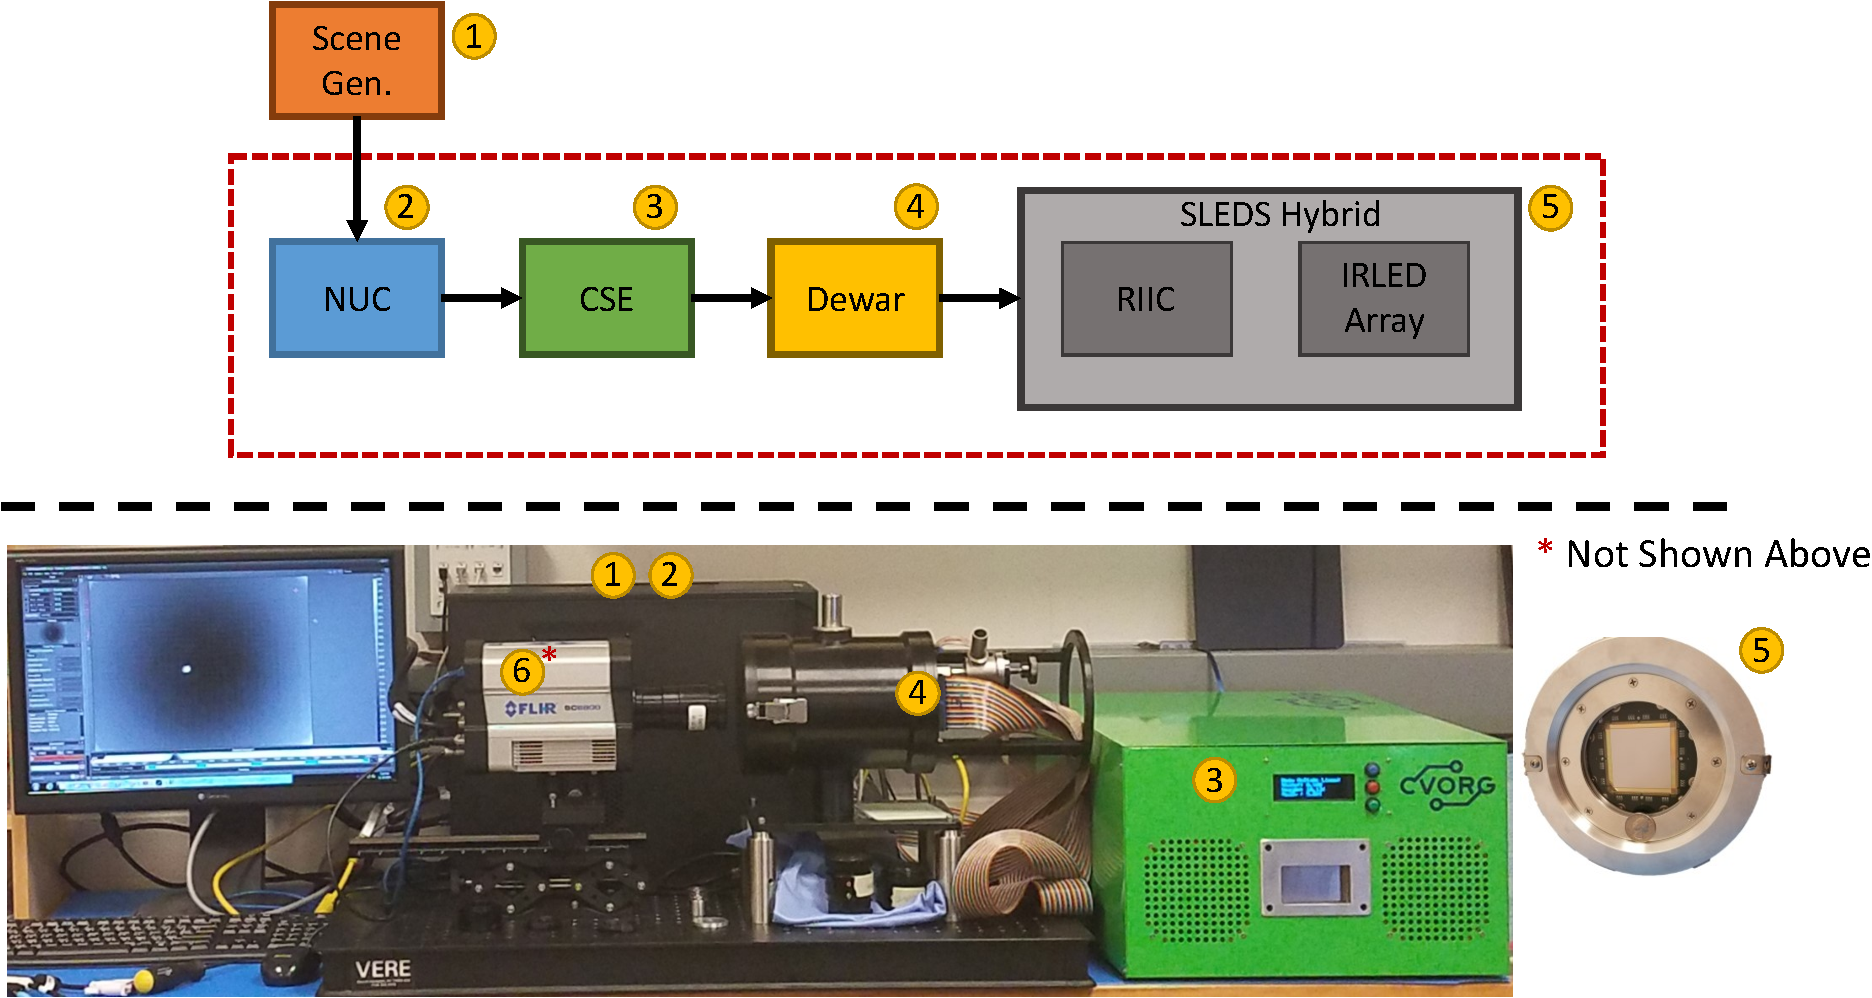
\includegraphics[width=1.0\textwidth]{fig/sleds_system.pdf}
        \caption{IRLED Scene Projector System}
        \label{fig:sleds_system}
    \end{figure}

    Figure~\ref{fig:sleds_timeline} shows the development timeline for IRLED IRSP technology. In 2008, the world's first IRLED array called the Superlattice Light Emitting Diodes (SLEDs) array was completed~\cite{AhmedEtAl2019}. This device was a hybridized combination of a 68 by 68 IRLED wafer bonded to a RIIC wafer~\cite{DasEtAl2009} providing the electronics to drive the array. Initial testing was done by hand prior the design and implementation of the overall drive system which was completed in 2011. Following this, an increased IRLED wafer of 512x512 size was fabricated in 2014~\cite{NortonEtAl2013}. The combination of the array with the drive system resulted in SLEDS (Superlattice Light Emitting Diode System), the first functioning IRLED IRSP system in the world. Further efforts culminated in two IRLED IRSPs in 2016. The first, TCSA (Two Color SLEDS Array), a 512 by 512 sized array~\cite{McGeeEtAl2015, EjzakEtAl2016, EjzakEtAl2016_2, EjzakEtAl2017, RickerEtAl2017} included support for driving the LEDs at two separate wavelength bands, denoted as 2-colors in Figure~\ref{fig:sleds_timeline}. The second, NSLEDS (N\footnote{The N originally stood for Nightglow, before the device was retargeted to Midwave-IR.} Superlattice Infrared Light Emitting Diode System), a 1024 by 1024 sized array~\cite{BenedictEtAl2017,AhmedEtAl2020} doubled the total number of pixels supported. Additionally, these systems demonstrated the beginnings of a modular IR Scene Projection (IRSP) platform~\cite{BrowningEtAl2019}. A further increase in size and efficiency occurred in 2018 with the world's first 2048 by 2048-pixel array, HDILED (High Definition Infrared LED)~\cite{BenedictEtAl2018}. A visual representation of the pixel ratios is shown in Figure~\ref{fig:tcsa_nsleds_hdiled_array_ratio}

    \begin{figure}
        \centering
        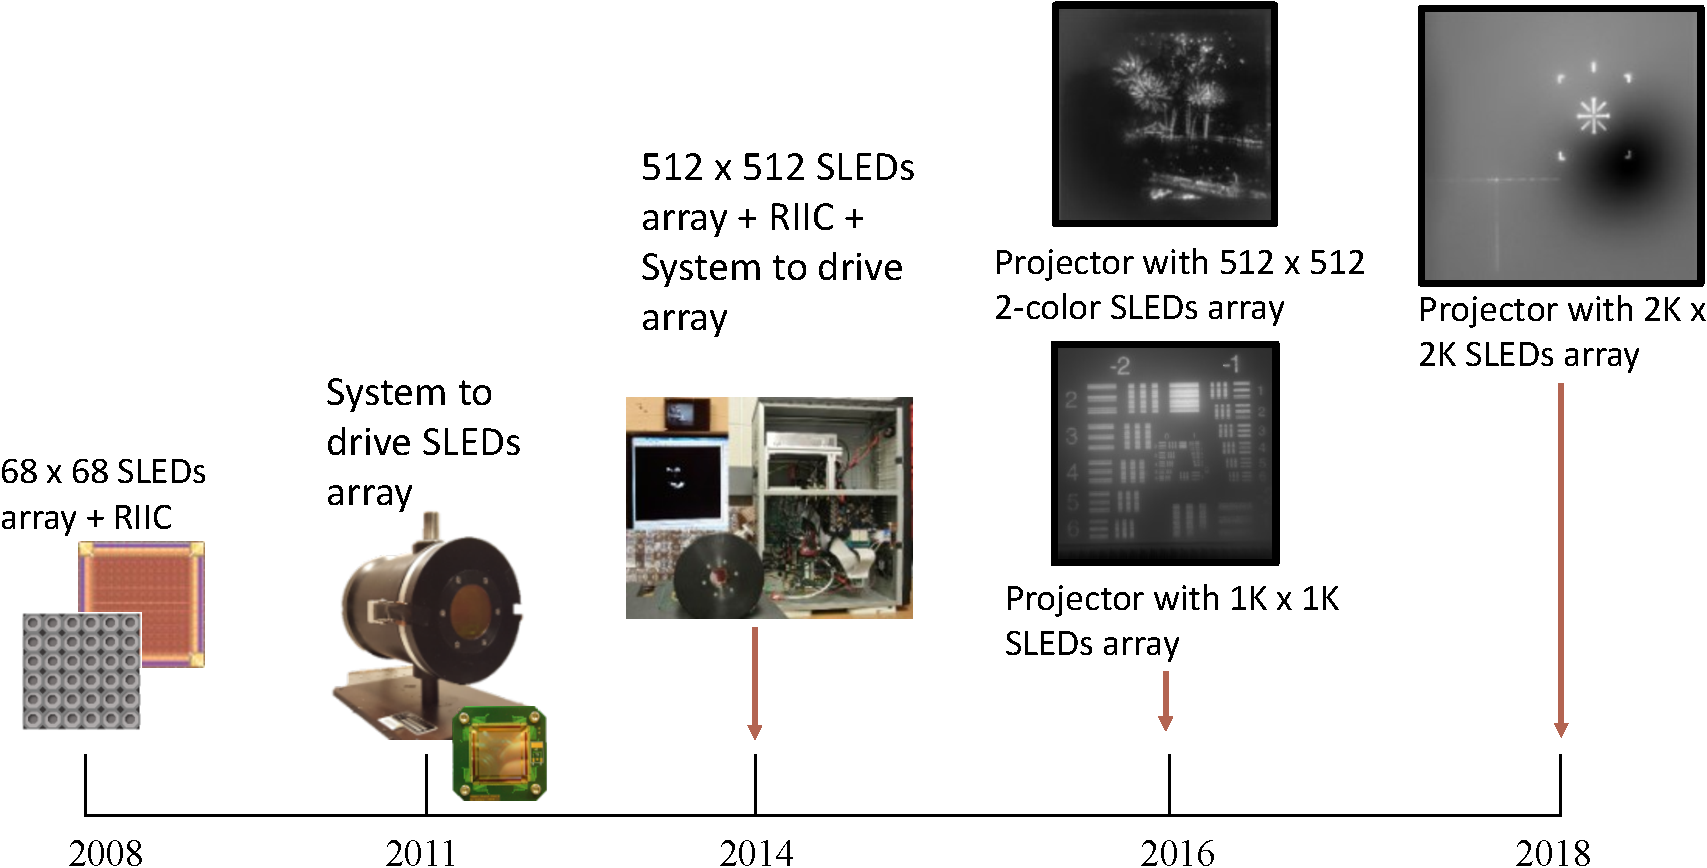
\includegraphics[width=1.0\textwidth]{fig/sleds_timeline.pdf}
        \caption{IRLED Scene Projector Technology Development Timeline Overview}
        \label{fig:sleds_timeline}
    \end{figure}

    \begin{figure}
        \centering
        %includegraphs[trim=L B R T]
        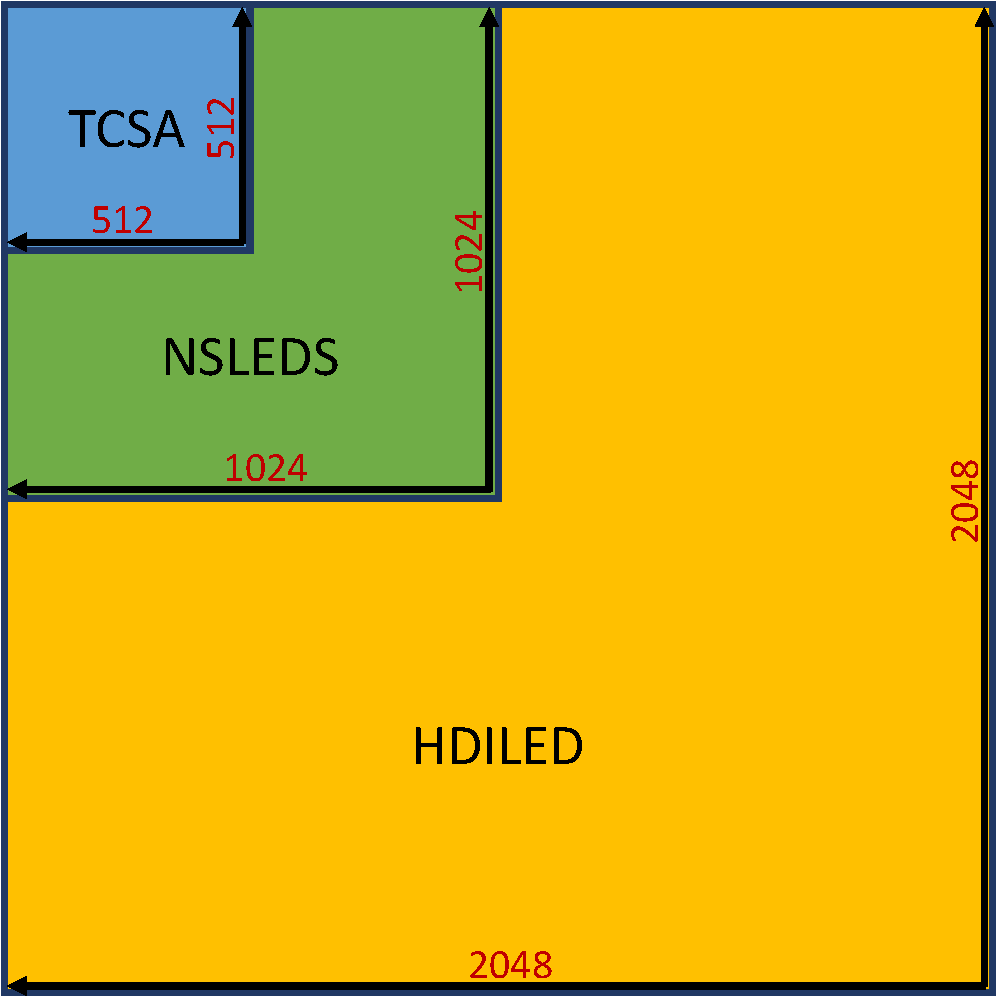
\includegraphics[width=0.5\textwidth]{fig/tcsa_nsleds_hdiled_array_ratio.pdf}
        \caption{SLEDs Array Pixel Ratios}
        \label{fig:tcsa_nsleds_hdiled_array_ratio}
    \end{figure}

    TCSA represented a novel step forward in terms of IRLED array technology. It incorporated a multiple color pixel design within a 1.3in\textsuperscript{2} package consisting of two overlayed LEDs per pixel to enable emission in multiple wave-length spectrums as well as an increase in the number of analog channels from 4 to 16 to allow for more pixels to be driven at a time. It targeted a speed of \mbox{1 kilohertz} operation. NSLEDS used the same size wafer as a TCSA, but decreased the pixel pitch from 48 to 24 microns and incorporated a single-color pixel design instead of the multiple color design of the original, these changes allowed for the pixel resolution to be doubled paving the way toward larger format IRLED IRSPs. Additionally, NSLEDS targeted \mbox{500 hertz} operation. HDILED increased the package size to 2.3in\textsuperscript{2} and doubled the resolution while utilizing a similar RIIC architecture to the prior two arrays. It targeted \mbox{250 hertz} operation. The interleaved write process of each array is discussed in detail in Chapter~\ref{sec:array_Interleaved_write_process}.

\section{IRLED Projection Process}
    Figure~\ref{fig:typical_projection} shows a typical projection process utilized within an IRLED IRSP. Each step operates at a static frame rate. A scene projector performs scene generation by utilizing a GPU typically. Following this, imagery undergoes non-uniformity correction by utilizing a NUC table created by analyzing the non-uniformity on a given array. After which, image data is reordered for sending to an array. When data is sent, a digital to analog conversion occurs for each value displayed on a projector.

    \begin{figure}
        \centering
        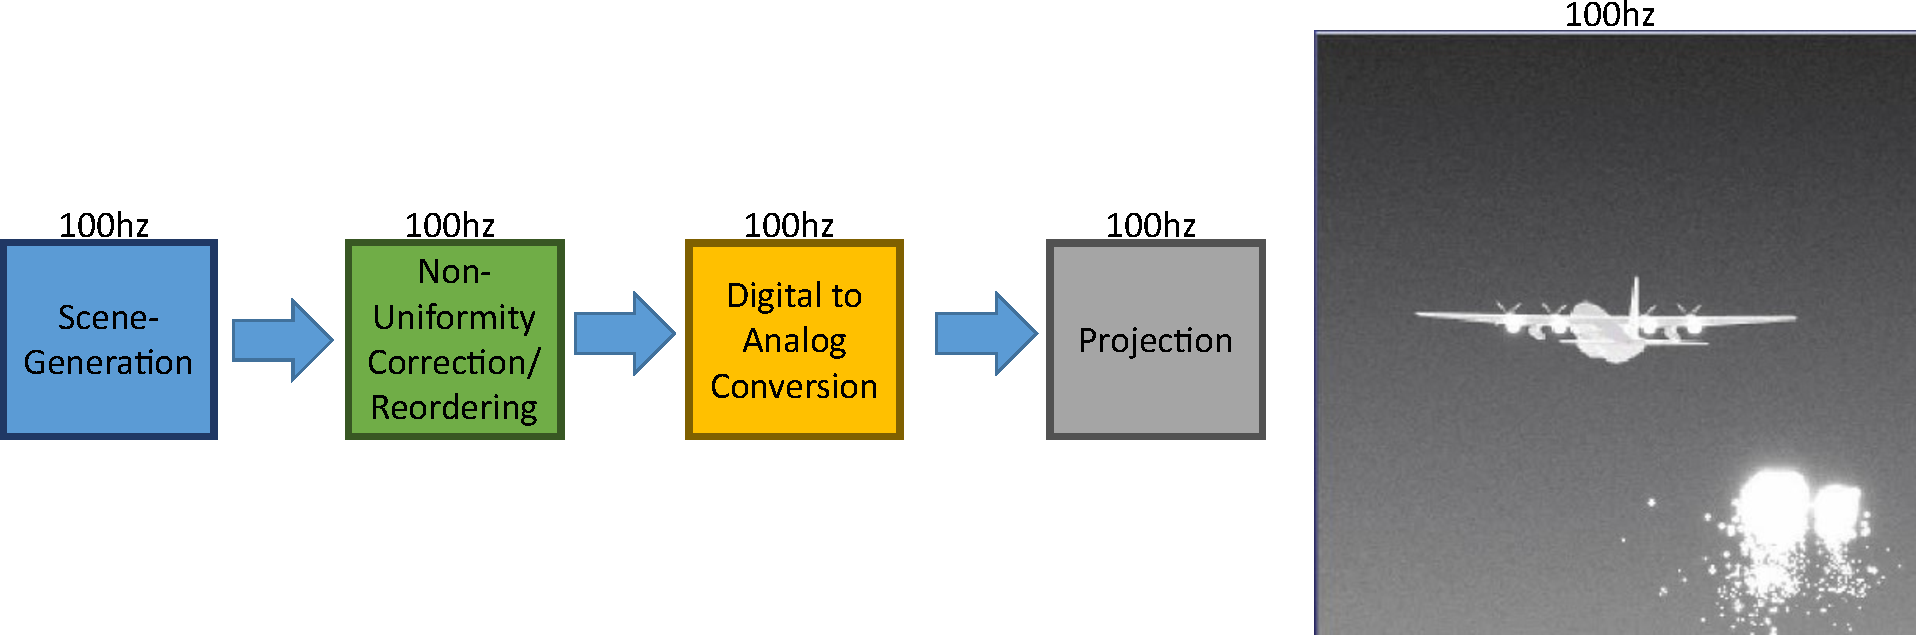
\includegraphics[width=1.0\textwidth]{fig/typical_projection_system.pdf}
        \caption{Typical IRLED Projection Process}
        \label{fig:typical_projection}
    \end{figure}

    The NUC process compensates for any physical defects that may cause non-linear variation in light emission from different diodes on a given array, thus, allowing for uniform emission across a given spectrum. There are number of different ways this linearization may be performed~\cite{BrowningEtAl2016, LandwehrEtAl2017, BarakhshanEtAl2018_2, BarakhshanEtAl2019, BarakhshanEtAl2019_2}, the details of which are beyond the scope of this work. After non-uniformity correction, imagery is converted pixel by pixel from digital to analog to drive the physical pixels at a given intensity on the array.

    The design of the digital to analogy chain of an IRLED IRSP is another important challenge as the analog bandwidth\footnote{The rise and fall time of digital-to-analog (DAC) conversion and amplification.} plays an important role in determining the maximum speed a system can operate at as well as the bit resolution\footnote{A measurement of to what degree changes to DAC inputs can produce consistent measurable light output differences.} of an array~\cite{EjzakEtAl2019}. Additionally, timing variance and potential differences in performance between analog channels needs to be analyzed and minimized through design and tuning. While outside of the scope of this work, it is worth noting that, a poorly behaving analog chain can introduce undesirable non-linear distortion in analog signaling resulting in non-linear projection ~\cite{Freeman1977, Gordon1978, ChanEtAl2008}.

    Similarly, the internal analog timings of an array's RIIC plays a critical role in this as well. One that may be considered even more crucial given that once an array is fabricated and bonded, it cannot be later modified. In contrast, a faster and more precise analog chain could be implemented at a later point in time for an existing array. Decisions made on RIIC architecture can have lasting long-term impact.

    The following chapter moves to a discussion of the central problems with display protocol technology and the proposed solution.

    \chapter{Problem Formulation}
        \label{chap:problem_formulation}

This chapter discusses in detail the limitations with current display protocol technology that were alluded to in Chapter~\ref{chap:introduction}. From there, it focuses on how these limitations affect adversely IRLED projector technology. Finally, it provides a problem solution.

\section{Display Protocol Limitations}

    Current display technologies, such as HDMI, assume a fixed frame rate display which places a hard limit on frame timing and synchronization.

    % Limitations:
    % Synchronization:
    %   -Implementation and integration-costs $
    %   -System-specific solutions $
    %   -Poor upgradeability $
    In detail, display protocols operate in a best-effort fashion where a buffer swap-initiated transfer of frame data occurs at a static predetermined interval. If a new frame is unavailable to be transmitted at each interval due to any delay, such as processing delay, the previous frame will be retransmitted. This necessarily makes correct synchronization challenging because modern computation systems do not generally provide real-time guarantees due to variability in system operation, including frame generation, CPU scheduling, and Input/Output (I/O) delays. Generally, while these challenges can often be addressed to some degree, they require custom hardware solutions on top of existing display protocols because end-to-end system synchronization is out of the scope of typical display standards which are designed to push relatively low frame rates over single hardware links. These solutions also tend to lack abstraction layers which can greatly hinder upgradeability.

    % Limitations:
    % Display Protocols
    %   -Frame rate limits                 -> image size inversely proportional to speed $
    %   -Static Bandwidth Requirements     -> full image transfer $
    %   -Static frame rates                -> 60Hz, 100Hz, etc. $
    %   -Scalability                       -> single scene generator, projector driver $
    %   Diagrams: Bandwidth diagram -- referenced already $
    Moreover, because of the static nature of the transmission interval (e.g. 100Hz), the frame rate cannot be dynamically controlled or changed after initialization. Instead, these protocols have static bandwidth requirements for a given resolution and frame rate of the form found in Table~\ref{tbl:bandwidth}, which shows that resolution size is inversely proportional to the max speed the display can operate at. Additionally, these protocols only support sending the entire frame at a given interval even if only a small portion of the frame has changed. This is a non-optimal use of bandwidth that does not allow for fine-grained control over the frame rate in cases where a user might wish to dynamically change the frame rate to match the processing rate. In high-speed display scenarios, this inevitably causes dropped frames. This issue is further compounded by the fact that conventional display protocols utilize proprietary drivers and hardware such that frame-drops become effectively silent. Similar to the synchronization solutions discussed above, this tends to lead to upgradeability issues due to systems being tailored for specific display hardware. This contributes to scalability issues as well since changing the display hardware often requires a complete system redesign.

    % Analog Chain:
    %   -RT settling time limitations: -- not included right now
    % Existing diagrams:
    %   Diagrams: scene generator -> Non-uniformity Correction -> Projector
    %   Diagrams: Modeline Overhead diagram

    \begin{table}
        \centering
        \large
        %\begin{small}
        %$$bandwidth = resolution \times bits \times fps$$
        %$bandwidth$ : \quad bandwidth requirements in bits per second. \\
        %$resolution$ : \quad number of pixels including porches. \\
        %$bits$ : \quad \quad \quad \ \ \ bits per pixel. \\
        %$fps$ : \quad \quad \quad \ \ \ frames per second.
        \begin{tabular}{| r l |}
            \hline
            $bandwidth$ & = resolution $\times$ bits $\times$ fps \\ \hline
            $bandwidth$ & : bandwidth requirements in bits per second. \\
            $resolution$ & : number of pixels including porches. \\
            $bits$ & : bits per pixel. \\
            $fps$ & : frames per second. \\
            \hline
        \end{tabular}
        \caption{Bandwidth requirements of a conventional display protocol}
        \label{tbl:bandwidth}
        %\end{small}
    \end{table}

\section{High-speed IRLED Scene Projector Systems}
% How these limitations affect IRSP
% Bottlenecks:
% Hardware limitations:
%   -Physical interconnect bandwidth and latency -> Concurrency/Parallelization $
%   -FPGA/ASIC/IC clock rates                    -> Concurrency/Parallelization $
%   -Analog chain settling times (DAC)           -> Address only the pixels needed $
% Software limitations:
%   -Computational/algorithmic limitations       -> Concurrency/Parallelization $
%   -Poorly optimized software / drivers         -> Do not use $
%   -Fixed frame display                         -> Dynamic frame rate + frame segmentation $
%   -Non-RT scheduling                           -> Realtime schedule / DMA -- not covered below - do i want to cover this?
%   -Lack of control                             -> Use a communication protocol with dynamic control built-in $
%

    Conventional display protocols, which are designed for driving relatively low speed consumer electronics as indicated in Chapter~\ref{chap:display_protocols}, are often utilized in High-speed IRLED IRSP systems. This results in a combination of unnecessary hardware and software limitations being incorporated into systems. This section will discuss these limitations and the general methodology toward alleviating them. Hardware limitations will be discussed first then software limitations.

    \subsection{Hardware Limitations}
        There are several hardware limitations including physical bandwidth, latency, IC clock rates, and analog chain settling times. Often the hardware that data is transferred over within these systems has inherent bandwidth and latency limitations that cannot be overcome either due to the nature of physics or simply because faster hardware is not available. One solution toward working around bandwidth issues is to introduce more parallel links into a system. A similar issue arises with respect to the clock rates of components within a system, such as, projector driver firmware, and scene generator. Ideally, these components will operate as fast as possible, but the reality is that the large fan out of I/O signaling needed by arrays can cause critical timing closure issues within FPGA based firmware implementations. Careful routing and planning can help alleviate these issue as well as parallelizing projector drivers such that less signals are driven from a single FPGA component. The speed of the analog chain in these systems is dictated by the digital to analog converter (DAC) and amplifier settling times which can be alleviated by increasing the number of converters utilized within a system if supported by an array. This could increase write speeds by allowing more DACs and amplifiers to drive smaller portions of an array in parallel. All the solutions discussed in this section involve increasing the number of parallelized components operating within a system in order to reduce physical bottlenecks.

    \subsection{Software Limitations}
        In terms of software, computational and algorithm limitations exist in the generation of scenery for display, and in correcting for pixel and array imperfections as well as in putting data into the correct format to be understood by a projector's driving firmware. Rendering of individual frames of a scene can be particularly computationally expensive. This can be further complicated by poorly optimized software drivers or algorithms. Additionally, in these systems, tight control over timing is important because frame drops are not tolerable. Meaning that fixed rate display technology is a hinderance in terms of user level control. One solution is to utilize technology that allows for dynamic frame rates and frame segmentation, which, requires protocols with dynamic control built in.


\section{Problem Statement}
    IRSP systems need to be capable of operating at high speeds with large resolutions to meet the needs of the sensor testing community. Typically, this can be on the order of 2048 by 2048 pixels with up to 1KHz frame rates with subframe latency. Necessarily, these goals represent a challenging problem to overcome when utilizing typical display technology which is further hindered due to the limitations discussed above. Given these constraints, the question what an appropriate solution is to address the aforementioned issues arises. The central question we could ask ourselves is, how to architect a generalizable, dynamic, and scalable IRSP system capable of High-performance operation, sub-frame latency, dynamic frame rates, and dynamic bandwidth utilization?

\section{Problem Solution}
    Within the current display protocol technology, any effort to address the aforementioned issues requires system developers to have complete control over an entire end-to-end system for a given solution to operate correctly. This means that in practice customized hardware and software that deviates from standard display protocol behavior is required. Any solution that lacks these requirements would fail to completely address operational issues with performance.

    In short, to truly address issues within the conventional display protocol would require creating a new system specific protocol tied to specific custom hardware. Additionally, with this type of solution, it is still not possible to achieve true sub-frame latencies due to the nature of display protocols requiring transmission of entire frames of data at a given interval or frame rate. In practice, IR projector systems are often forced to introduce intermediate buffers within a system in order to ensure correct operation.

    I believe that any effort to address the aforementioned issues and answer our problem statement requires developing a hardware agnostic alternative display protocol designed specifically for high-speed low-latency frame transmission. This would allow for the protocol be retrofitted within existing systems as well as allow for upgradeability, and support for future hardware. In order, to achieve sub-frame latencies, this protocol would need to support transmission of sub-frames of data, i.e. transmission of partial frames. Allowing for partial frame transmission enables a host of other desirable features, such as, the ability to control bandwidth utilization and the ability to incorporate dynamic frame rates. A good method of supporting partial frame transfer is to utilize headered packets of data to provide a context for what the data represents and where to draw said data on a display. This method of transferring display data is called a packetized display protocol (PDP).

    As discussed briefly in the Chapter~\ref{chap:introduction}, this PDP architecture eschews with assumptions found in conventional display technologies to provide a robust feature-set. In contrast to a normal display protocols, the proposed architecture, is designed to utilize a dynamic source driven refresh rate through the coordination of both source (scene generator) and sink (display). In this architecture, frames are segmented into pieces and sent to the display based upon how often these segments need to update. An example of this is shown in Figure~\ref{fig:variable_display} where different regions of the display operate at different frame rates. By utilizing dynamic frame rate control at sub-frame resolutions, substantial bandwidth reductions can occur. This will be discussed in further detail in Chapter~\ref{chap:pdp_protocol}.

    \begin{figure}
        \centering
        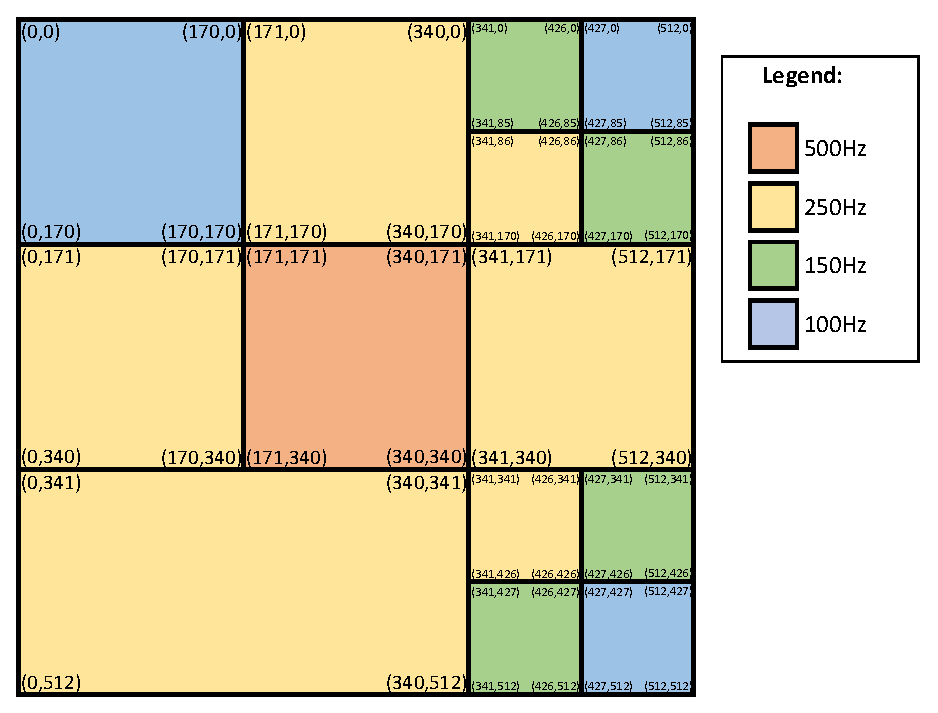
\includegraphics[width=1.0\textwidth]{fig/variable_display.pdf}
        \caption{Dynamic frame rate display with multiple regions updating at different frame rates}
        \label{fig:variable_display}
    \end{figure}

    The underlying PDP itself is designed to allow for fine-grained control over when and what data is transmitted as well as to incorporate mechanisms to synchronize displays. Furthermore, the protocol architecture is abstracted in such a way that the physical interconnect layers are transparent in order to enable it to be capable of operating over a wide-spectrum of hardware as well as to allow the protocol to be extended and used within future hardware. For system upgradeability, this offers a risk reduction because it allows for a simpler migration path as new hardware becomes available. For example, a hardware system implementing this protocol could switch or upgrade physical components and still utilize the same protocol within the software stack given an appropriately compatible physical layer. To further facilitate this, a packetized protocol structure capable of transmitting pixel data in a generalized way has been chosen. These details will be discussed in Chapters~\ref{chap:pdp_protocol} and~\ref{chap:machine_model}.

    The remainder of this work is devoted to discussing the details of the environment in which the PDP is designed to operate, the protocol itself, and its implementation. The following chapter provides an overview of system operation.

    \chapter{System Overview}
        \label{chap:system_overview}
This chapter provides the reader with an overview of IRLED electronics. Firstly, it discusses the Close Support Electronics (CSE)\cite{EjzakEtAl2015,HernandezEtAl2019,SinghEtAl2020} hardware used to drive IRSP systems in order to give the reader an understanding of the internal flow of data from entry into a CSE to output to an external array. Following this, it discusses the communications within a CSE at a block level to provide the reader with an understanding of how communication flow works within a CSE for configuration. Finally, external communication of an overall IRLED system is discussed at a block level to provide the reader with a high-level understanding of the flow of communication from input (scene generation) to output (array) in different system configurations.

\section{Close Support Electronics}
    \label{sec:close_support_electronics}
    As mentioned briefly in Chapter~\ref{chap:background}, a CSE is needed to drive IRLED arrays. Conceptually, A CSE is an interface that converts digital display data to an array specific format in order to produce IR imagery. From there it converts formatted data from the digital domain to analog and amplifies analog signaling to drive an array by charging the internal array cells that make up an array. It further provides power for an array, and regulates the current in order to safeguard arrays from physical damage due to misconfiguration, heating, or hardware faults.

    The TCSA, NSLEDS, and HDILED arrays discussed in Chapter~\ref{chap:background} can all be driven using the same electronics with the only difference in the boards directly attached to the hybrid array. Figure~\ref{fig:sleds_block} shows the internal components of the CSE architecture, called {\it Nessie}, broken out in green. In typical configurations, a display system drives a CSE using dual HDMI inputs to increase the system bandwidth and achieve higher frame rates. Typically, these will each carry half of a frame segmented either vertically or horizontally. Each input decodes the video signals in parallel and then outputs individual pixels that are then routed into the main FPGA board which houses a Xilinx Vertex 6 FPGA\cite{XILINX2015}. From there, pixels are routed into an internal buffered directly or decoded (in the case of PDP) and then buffered. Other interfaces may be utilized in place of HDMI as will be discussed later in this section.

    \begin{figure}
        \centering
        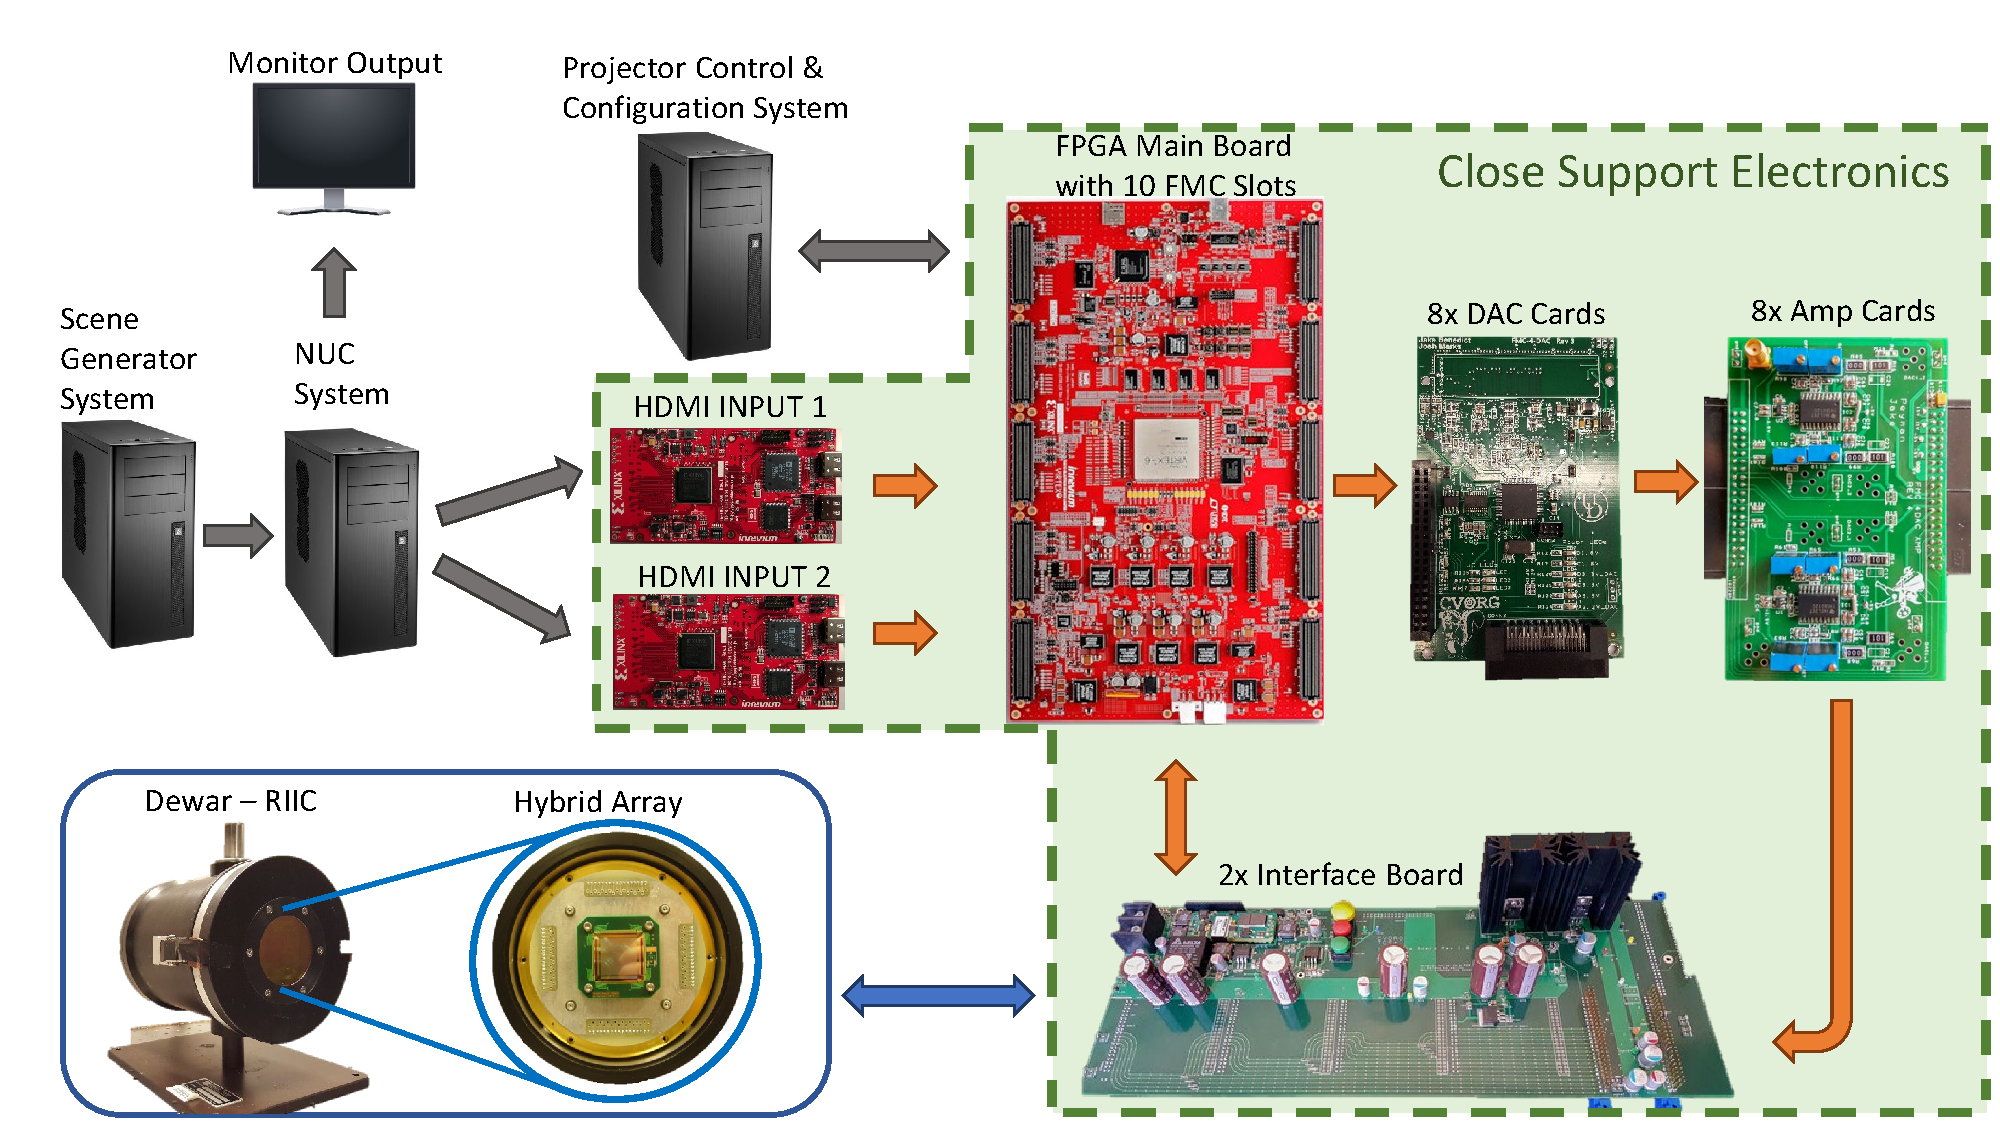
\includegraphics[width=0.67\textwidth]{fig/sleds_block.pdf}
        \caption{SLEDS System Block Diagram}
        \label{fig:sleds_block}
    \end{figure}

    Due to the two input cards, the firmware within the main FPG board is responsible for multiplexing between both inputs to draw data to an array without allowing for the internal firmware buffers to overflow. In practice, current firmware does this by buffering the minimal amount of data needed for a write from both inputs in parallel and context switches between the inputs every other write or every two writes depending on the configuration. As long as the buffers are sized large enough to accommodate for the time needed for the array write process to finish for an individual write, then overflow should not occur. Additional logic is provided to query and detect internal buffer overflows in cases of misconfiguration or signal integrity faults. In practice, if an overflow fault occurs, it is visually obvious in recorded IR data as well.

    Once enough data is buffered for one of the inputs, the firmware will control the write process to drive the 8 DAC cards which each house 2 16-bit DAC integrated circuits per card, with each circuit consisting of 2 channels per DAC. Yielding 32 parallel channels with 512 total signals. Once the DAC process is done, the analog output of the 32 channels is then routed to 8 amplifier card which contain 4 amplifiers each. Following this, the amplified signals are routed through 2 interface boards which contain ribbon cables that attach to an array hybrid. The ribbon cabling carries both the amplified signals as well as other control signals from the firmware that are routed directly from the main FPGA board to one of the interface boards.

    Figure ~\ref{fig:round_board} shows an example of a circuit board which ribbon cables would be attached to via receptacles (not shown). Four ribbon cables can be attached to bring signaling to an array.

    \begin{figure}
        \centering
        %includegraphs[trim=L B R T]
        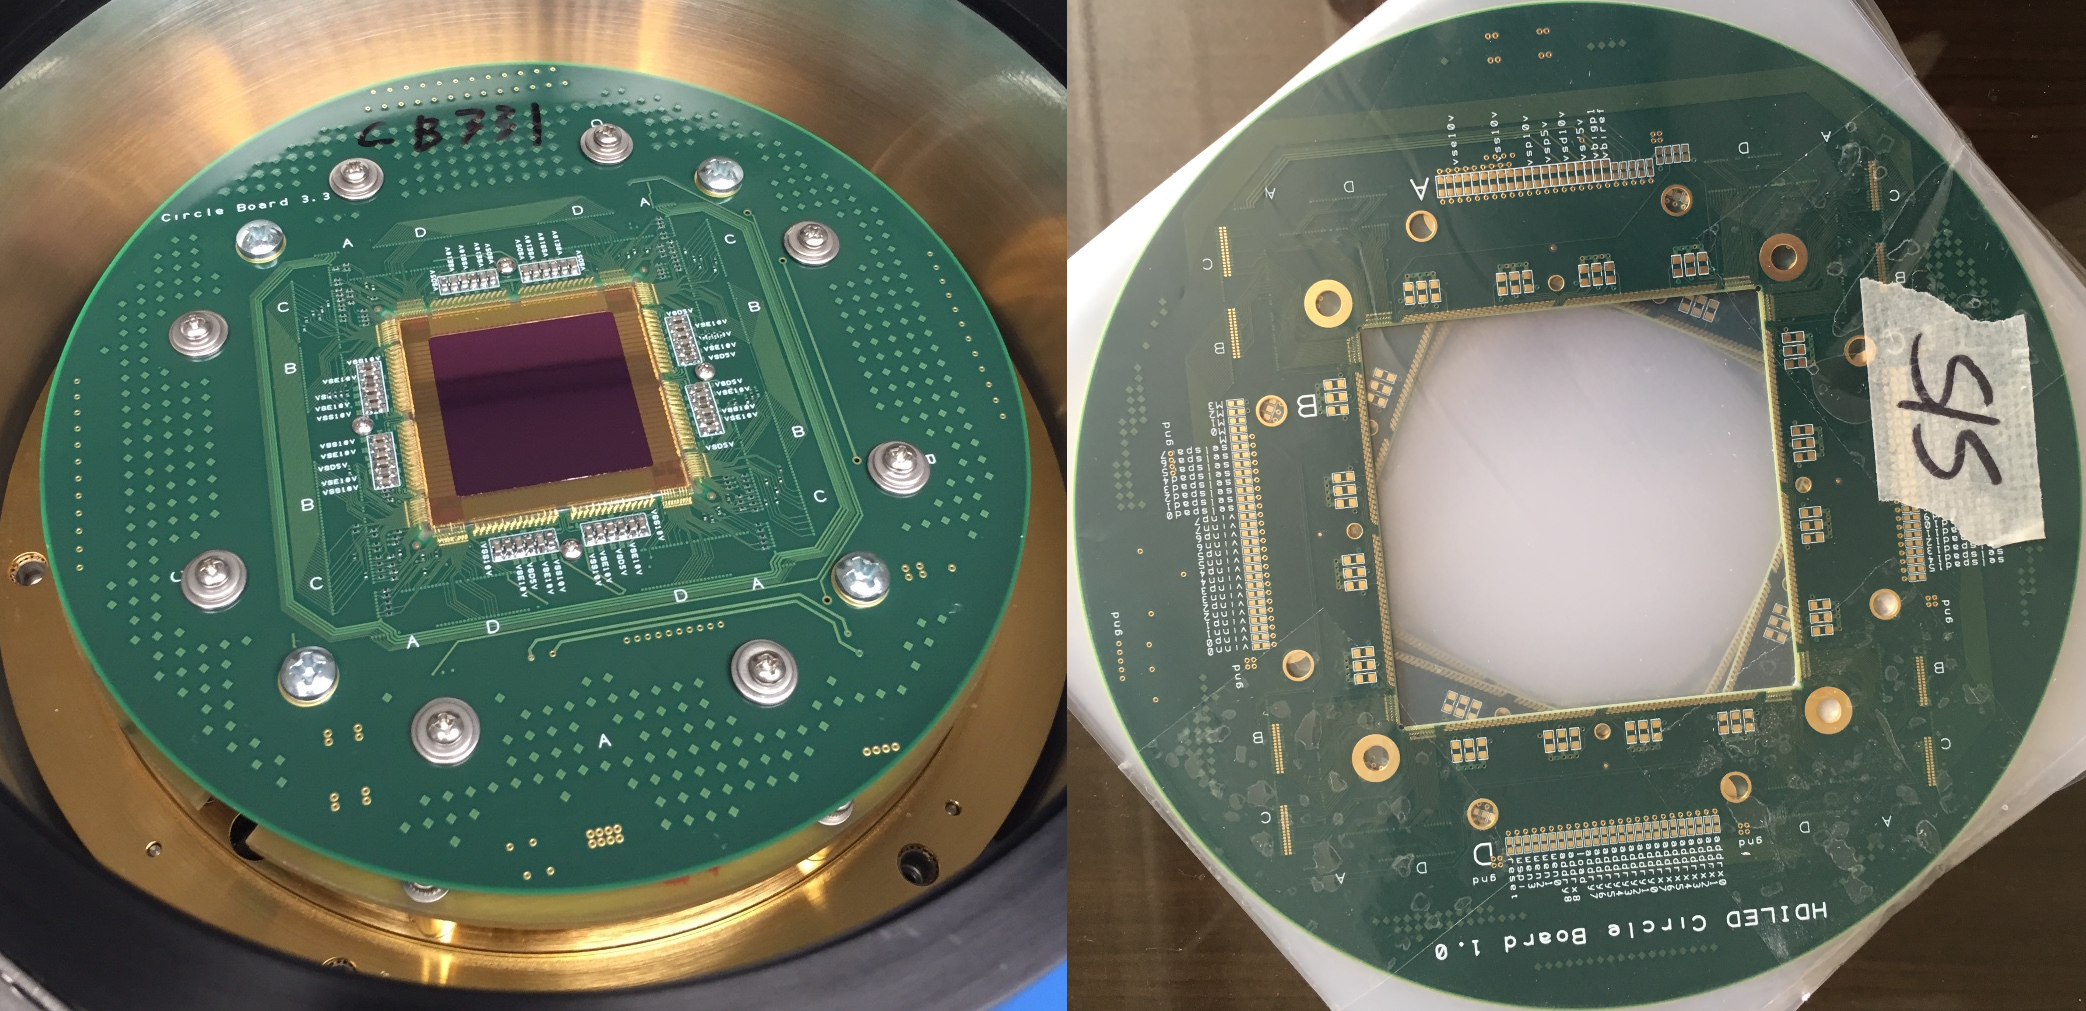
\includegraphics[width=1.0\textwidth]{fig/round_board.png}
        \caption{Example Hybrid Round Boards}
        \label{fig:round_board}
    \end{figure}

    Figure~\ref{fig:nessie_enclosure_internals} shows the components installed within a CSE chassis. Multicolored ribbon cables are shown in the top right. Mounted to the bottom is the main FPGA board. The two large boards at the top are the 2 interface boards with 8 amplifier cards plugged into them along the bottom. The boards in between the FPGA and amplifier cards are the DAC cards. The power supply is on the left.

    \begin{figure}
        \centering
        \includegraphics[width=1.0\textwidth]{fig/nessie_enclosure_internals.jpg}
        \caption{CSE Internals}
        \label{fig:nessie_enclosure_internals}
    \end{figure}

    The additional control signals provided by the firmware and routed to the RIIC through these cables are discussed in Chapter~\ref{sec:array_Interleaved_write_process}. The specifics of the PDP firmware architectures write process are discussed in Chapter~\ref{chap:implementation}.

    Figure~\ref{fig:nessie_enclosure_externals} provides an external view of a newer CSE chassis that is colored green to follow the {\it Nessie} architecture name as well as a view of the inside of the chassis when the majority of components aren't installed.

    \begin{figure}
        \centering
        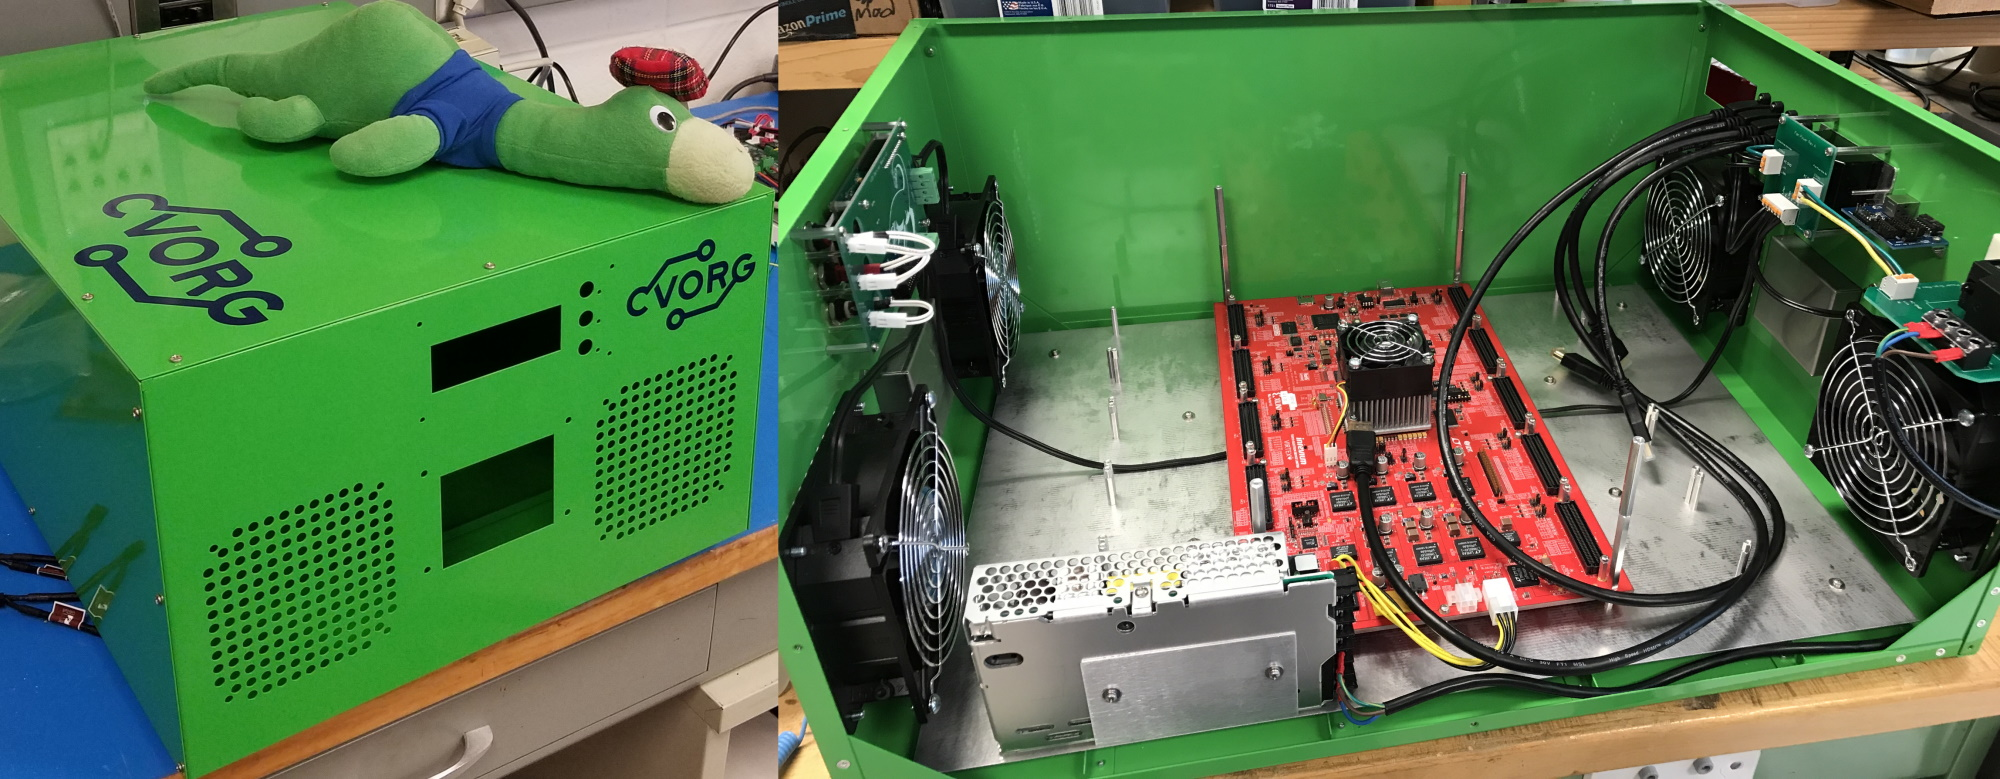
\includegraphics[width=1.0\textwidth]{fig/nessie_enclosure_externals.png}
        \caption{CSE Externals and Empty Chassis}
        \label{fig:nessie_enclosure_externals}
    \end{figure}

\section{Communication Flow}
    In this section, a discussion of internal CSE communication will be provided followed by a discussion of external communication within an IRLED projector system as a whole.

    \subsection{Internal CSE Communication}
        Figure~\ref{fig:cse_comm_block} shows the internals of CSE communication. Communication for controlling the behavior of CSE is done through a daisy chained set of UART devices utilizing a reliable blocking two way communication protocol called the CVORG protocol\footnote{Named after my research group at the University of Delaware.}. Without loss of generality, the protocol itself consists of commands to control various aspects of operation, such as, tripping an array, setting voltage limits, and configuring firmware operation. It also allows for information to be retrieved about current system configuration as well as operational errors. The destination of an operation is encoded as part of each command. Thus, commands not meant for a given component are forwarded along the chain. When commands are issued by a system, they are encoded for transport via the CVORG protocol and sent over UART. The system will then wait for an acknowledgment potentially containing payload data. When a command has finished executing within a CSE, it will send the acknowledgment over UART to the command initiator with requested payload data or simply as a receipt indicating that an action has been successfully executed. The underlying implementation details of the CVORG protocol itself are beyond the scope of this work and will not be discussed here.

        Memory mapped I/O between the frontend and backend firmware is controlled by the Microblaze soft processor and used to control the underlying PDP firmware registers as well as program an array using Serial Peripheral Interface (SPI) (Not shown). The details of command operations will be discussed in Chapter~\ref{sec:frontend_arch}. Additionally, SPI communication is also used to send data for LCD readout. Typically, this includes voltage and current information as well as the results of power on sanity checks. Finally, the details of the processing performed on HDMI display data sent directly to the Backend Firmware within PDP will be discussed in Chapter~\ref{sec:backend_arch}. Earlier non-PDP firmware implementations utilized within the TCSA, NSLEDS, and HDILED arrays also utilized HDMI but contained a different less robust implementation. These are outside of the scope of this thesis and will not be discussed here.

        \begin{figure}
            \centering
            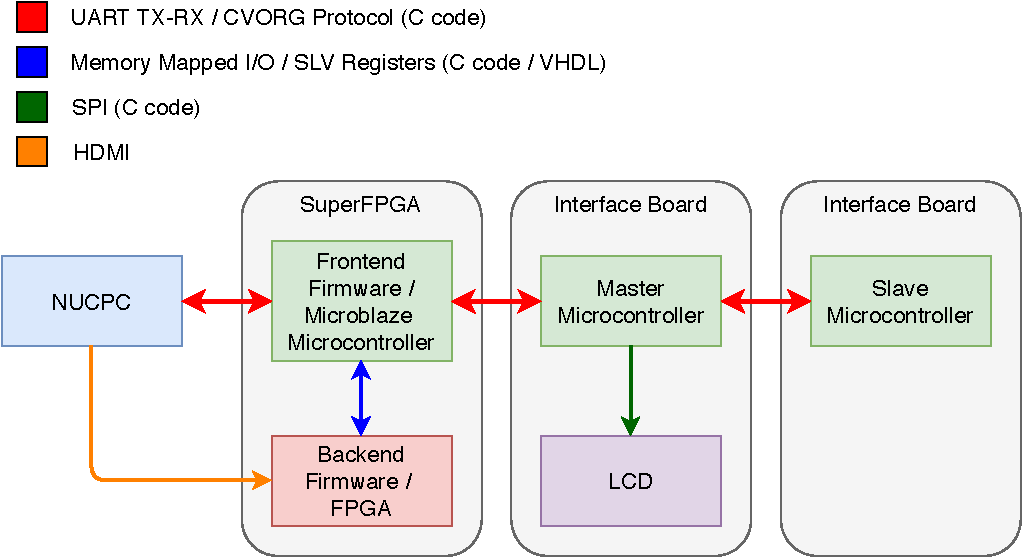
\includegraphics[width=1.0\textwidth]{fig/cse_comm_block.pdf}
            \caption{CSE Internal Communication Block Diagram}
            \label{fig:cse_comm_block}
        \end{figure}

    \subsection{External System Communication}
        Figures~\ref{fig:external_cse_comm_direct}, \ref{fig:external_cse_comm_half_indirect}, and \ref{fig:external_cse_comm_indirect} show the details of external communication to a CSE in various different system configurations. These provide a representation of some general types of setups that an IRLED array may be placed in. In general, a scene generator of some form would be utilized in all cases to provide IR scene imagery for an array to display. In all the configurations, a Low Pin Count (LPC) FPGA Mezzanine Card (FMC) connector provides the ability for various interfaces to be used to send data to the CSE, such as serial protocols or display based protocols over different types of hardware links. The FMC interface cards are responsible for retrieving the data over the link and formatting it in a manner that the internal CSE FPGA can decode.

        In practice, in display protocol setups, 24-bit pixel words and a data enable pin are utilized, but there is no hardware limitation and other word sizes could be used in setups that utilized other types of interfaces. A vertical sync signal can also be utilized to reset pixels every display frame in display protocol setups. As mentioned earlier in this section, current CSE setups utilize two HDMI FMC cards for input where the input for the top half of an array will be delivered over one cable and the bottom over the other.

        For example, in the NSLEDS array, input would be split into two 512 by 1024 display streams operating in parallel. API communication on the other hand utilizes UART and the CVORG protocol and is largely the same process for all arrays. Generally speaking, on start, frontend software would configure the firmware to output for the correct array size and program the array. After which, auxiliary functionality such as tripping and untripping the array would typically be the only strictly necessary communication done over UART.

        High-speed serial interfaces are currently in development in order to provide more control over the timing of data sent to CSEs within systems. These would allow for the blanking data inherit in display based protocols to be removed altogether\footnote{Blanking is discussed in Chapter~\ref{chap:display_protocols}.} as well as provide users with a means to send data only when required as opposed to at a strictly static interval controlled by vendor drivers such as is the case with GPUs.

        Figure~\ref{fig:external_cse_comm_direct} depicts direct communication in which formatted scene data is sent directly to a CSE and system configuration is done directly by a scene generator. In this type of setup, the scene generator can monitor CSE operation directly as well as operate in either a closed or open loop type setup\cite{NagrathGopal2009,Frank2018}.

        \begin{figure}
            \centering
            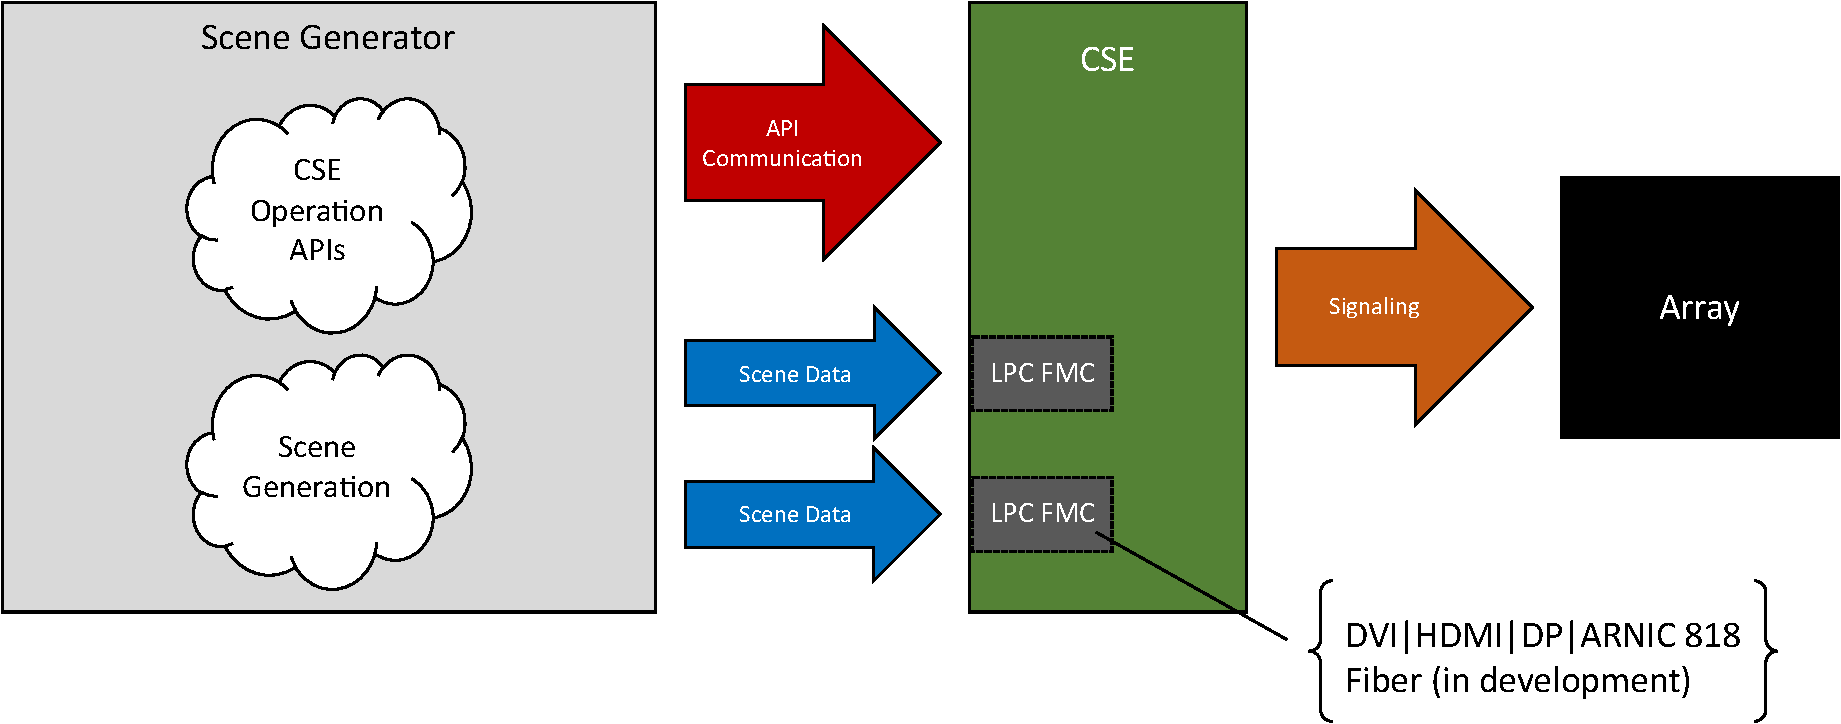
\includegraphics[width=1.0\textwidth]{fig/external_cse_comm_direct.pdf}
            \caption{CSE External Direct Communication Block Diagram}
            \label{fig:external_cse_comm_direct}
        \end{figure}

        A direct communication setup is desirable for minimizing end-to-end latency within a system for use cases where performance is paramount. For example, closed loop scenarios may feed recorded output imagery from an array back into the scene generator for in the loop analysis or in some cases subsequent frames may depend on the recorded results from prior frames. This means that in many cases subframe latency is desirable in that individual components in a system should not require buffering entire frames anywhere in the system as this would introduce a latency of a frame or more from generation to capture. This would necessarily result in the system needing delayed feedback control\cite{HuWang2002}. This represents a complex problem to solve in practice. It becomes even more difficult if the frame delays are unpredictable and dynamic from frame to frame forcing the scene generators to compensate in some manner, such as, sending off frames\footnote{An off frame is simply an empty frame that can be analyzed to check if frames are arriving at the expected time or if a frame slip or unexpected delay has occurred.} between imagery to characterize delay and detect unexpected behavior as well as provide a means of resynchronization between a scene generator and camera or sensor.

        Figure~\ref{fig:external_cse_comm_half_indirect} depicts indirect API communication in which system configuration is done through client APIs, and scene data is sent directly to a CSE. This type of setup is useful for situations where control over a CSE is needed but where API operation cannot be tightly coupled with a scene generator due to development costs or practical reasons. Similar to the direct setup, end-to-end latency is minimized by directly driving an array.

        \begin{figure}
            \centering
            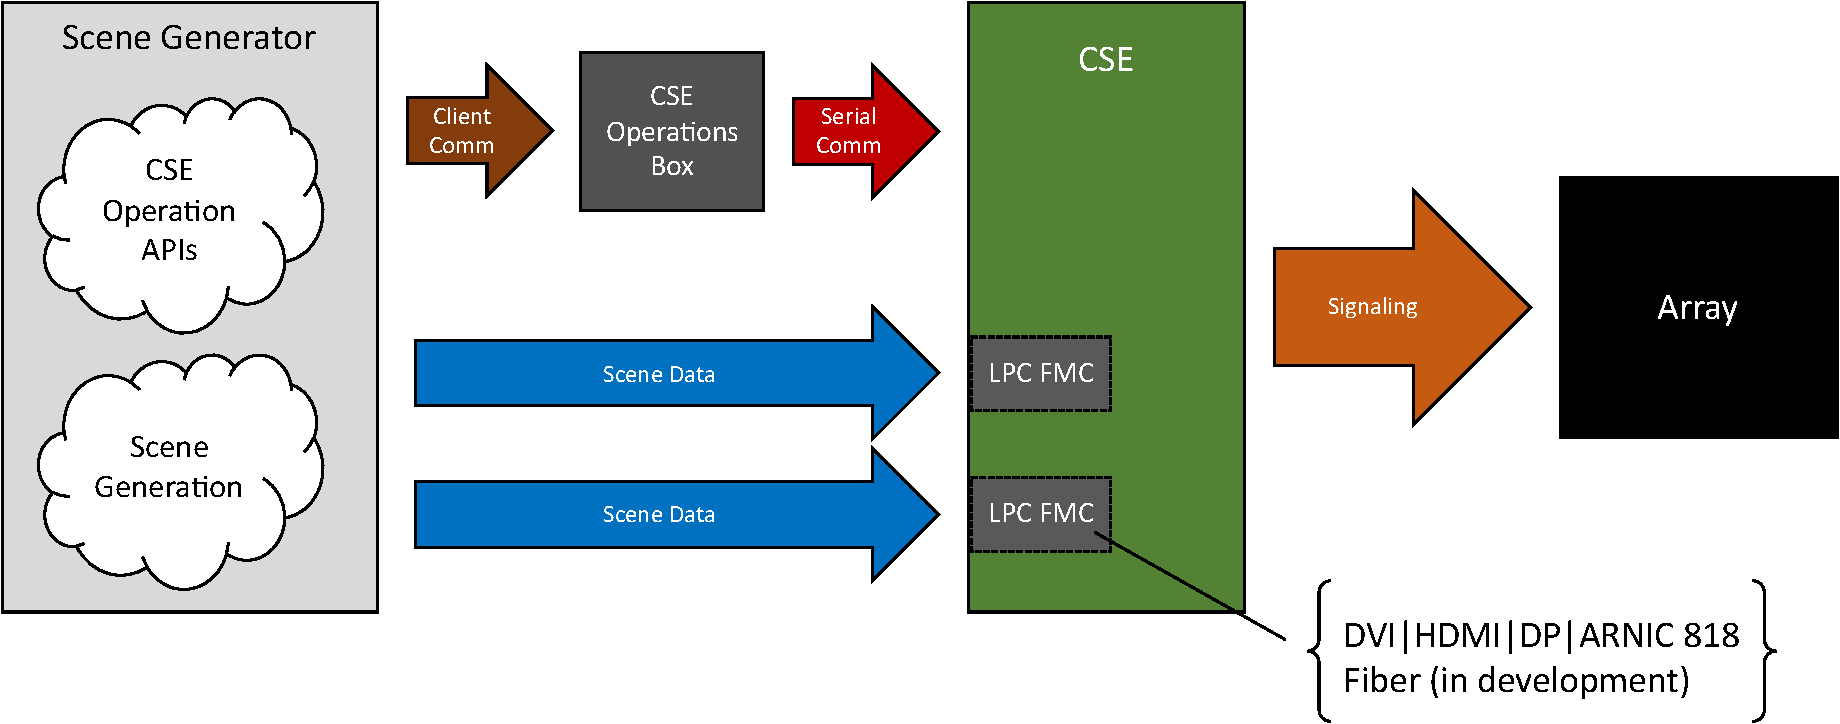
\includegraphics[width=1.0\textwidth]{fig/external_cse_comm_half_indirect.pdf}
            \caption{CSE External Indirect API Communication Block Diagram}
            \label{fig:external_cse_comm_half_indirect}
        \end{figure}

        In an indirect API communication setup, thin client API shims are provided to execute commands using remote procedure calls (RPC) which then are executed within a CSE operations box to communicate with the CSE\cite{CampbellEtAl2019}. This API shims provide the same interface and level of control as the direct API communication but are simply issued through some indirect layer such as Ethernet or InfiniBand. When a shim command is issued it encoded and transmitted to the CSE Operation Box. The CSE operation box then maps the shim command into a direct command call (as if it were being executed directly by a scene generator) and sends it to a CSE. Then the CSE operation box waits for a response from the CSE. Once a response has arrived from the CSE it will encode it and transmit it back to the scene generator, which is analogous to the direct operation of the CVORG with a middleman in between.

        Figure~\ref{fig:external_cse_comm_indirect} depicts an indirect setup in which both API communication and scene data are sent to an intermediate CSE operations box. Similarly, to the indirect API communication setup, client API shims are provided to execute commands using remote procedure calls (RPC) which then are executed within a CSE operations box to communicate with the CSE.

        \begin{figure}
            \centering
            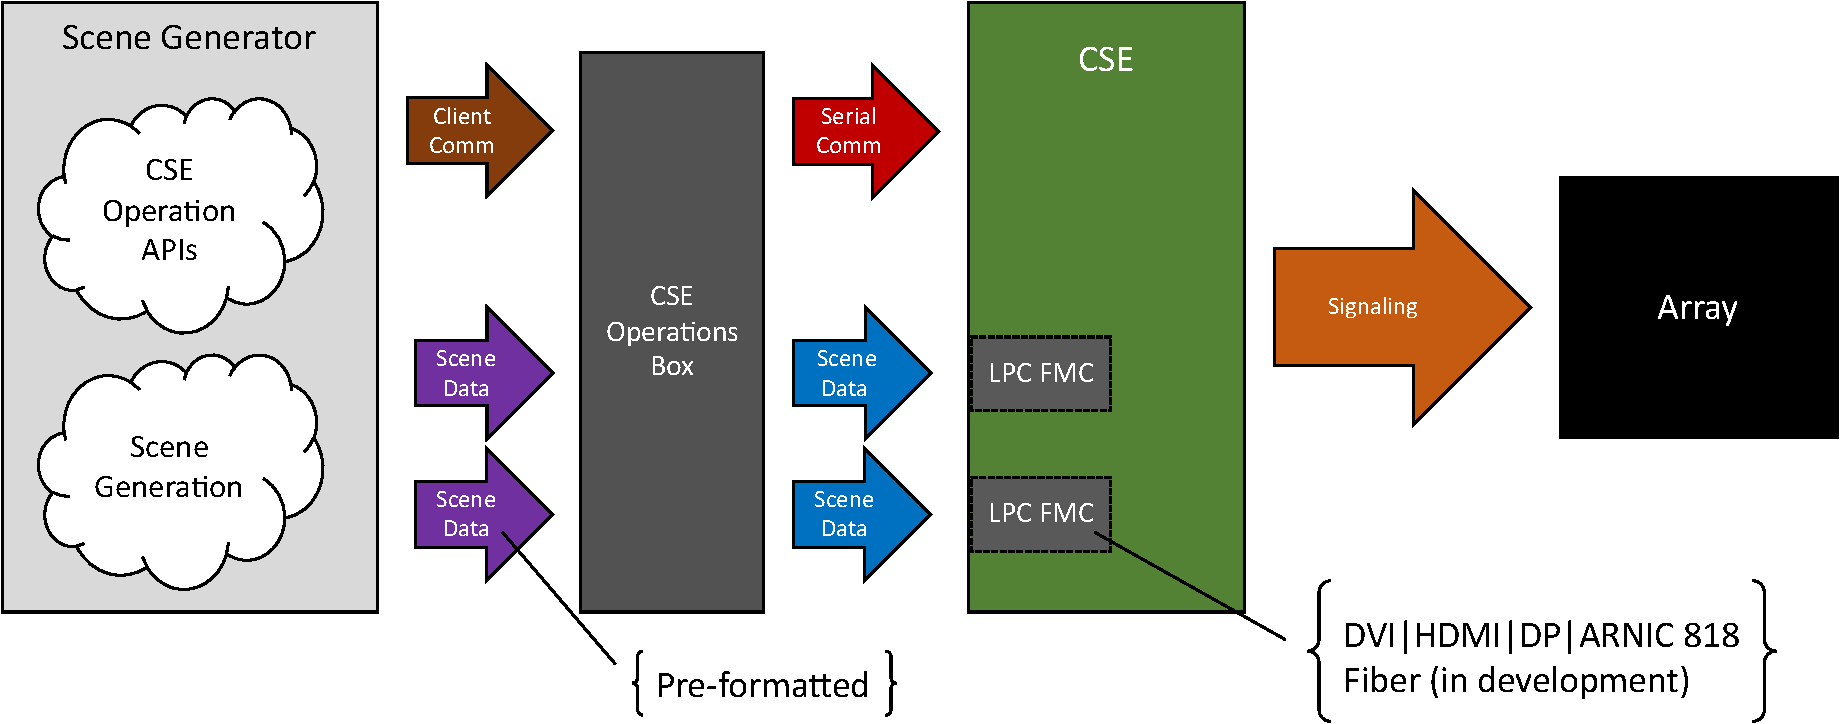
\includegraphics[width=1.0\textwidth]{fig/external_cse_comm_indirect.pdf}
            \caption{CSE External Indirect API and Data Communication Block Diagram}
            \label{fig:external_cse_comm_indirect}
        \end{figure}

        An indirect data and API communication setup is utilized in the event that data cannot be formatted directly for display on an array within a scene generator. It may also be utilized in cases where non-uniformity correction is performed externally from scene generation as shown in Figure~\ref{fig:sleds_block}. However, this would result in an additional latency cost that could complicate synchronization in closed loop setups due to delayed feedback control being required. A third scenario where this type of setup may be used is without a scene generator, where a CSE operation box could be used as a test bed to characterize an array directly as well as to test and troubleshoot operations. Imagery itself also could be displayed directly from the CSE operation box. This may be desirable in some open loop setups where the recording and processing of data is performed separately as this means no additional infrastructure would be required to be developed by users to interface with a CSE. Instead, users could utilize the provided infrastructure with little to no development costs.

        In closing, there are many different possible system setups in which IRLED projector systems can be utilized depending on user application and requirements. A well design IRLED system will ease the process of incorporating a new projector within an environment through versatility while minimizing performance impact as well as providing users with a clear picture of the tradeoffs associated with each type of setup.

        While this chapter covered the flow of communication inside and outside a CSE as well as different system setups in order to provide the reader with an understanding of the challenges and complexities of utilizing and driving IRLED arrays, Chapter~\ref{chap:array_write_process} shifts focus to discuss the hardware details of IRLED arrays' write process and the formatting of data sent to arrays to provide context on some of the challenges of writing to an IRLED array.

    \chapter{Array Write Process} % DONE
        \label{chap:array_write_process}
This chapter provides the reader with an overview of the data formatting required to drive an IRLED array, and hardware specific details of the underlying array write process to facilitate an understanding of the context in which the PDP is implemented as well as highlight some of the challenges with high-speed operation. Firstly, it discusses the interleaved write process required to directly drive LEDs on an IRLED IRSP. Then, it discusses the data re-ordering done to optimize the write process. Protocol level details of how external data is received are discussed in Chapter~\ref{chap:display_protocols}.


\section{Array Interleaved Write Process}
    \label{sec:array_Interleaved_write_process}
    Although all current IRSP arrays utilize display protocol technology that is decoded pixel by pixel to drive the emitters of an array, arrays may utilize different internal drawing mechanisms for driving pixels. This section discusses the details of those mechanisms within the TCSA, NSLEDS, and HDILED arrays for conceptual purposes, and while the details may differ for other arrays, the overall raster write process is generalizable in the sense that not all pixels are driven at once. Instead some subset of pixels is driven depending on how many analog channels can be utilized at the same time. The number of channels is largely dependent on the array design; however, in some cases the circuitry an array is mounted to allows for some configuration\footnote{Figure~\ref{fig:round_board} shows an example of supporting circuitry in Chapter~\ref{sec:close_support_electronics}}. For example, an HDILED array has 32 channels in typical configurations, meaning that it can drive 32 pixels at once. However, each quadrant can be operated independently with certain board setups, yielding up to a 128-channel maximum. Similarly, it can also be configured to utilize only 16 channels, 8 channels, 4 channels, and 2 channels as well. The details of these configurations are discussed in more detail later in this section.

    Arrays which operate in a snapshot mode also exhibit similar operational behavior. Snapshot mode is a type of array operation in high-speed projector systems in which light output does not occur until every pixel for a frame is written. It works by only transferring charge to embedded emitters once all pixel data is written~\cite{McHughEtAl1999}. This has the benefit of reducing heat variation across an array. However, the actual write process is very similar to non-snapshot operation which is often referred to as a rolling-update mode of operation within literature. Similar to rolling-update operation, each pixel charges either individually or in segments. The only difference is that the emitters themselves are enabled later. The write order and number of pixel segments driven at the same time is array dependent though.

    The TCSA, NSLEDS, and HDILED arrays are organized into four quadrants as shown in Figure~\ref{fig:tcsa_nsleds_hdiled_quads}. Each quadrant is organized into a given number of pixels with TCSA housing 256 by 256, NSLEDS housing 512 by 512, and HDILED housing 1024 by 1024 per quadrant. There are number of input signals necessary to drive an array. These are {\em a 4-bit quadrant write enable}, {\em X address}, {\em Y address}, {\em LOAD bit}, {\em 16 Strong/Weak drive strength bit}, {\em array reset bit}, and {\em analog signaling lines which charges the pixels being addressed}. The quadrant write enable, X address, Y address, and LOAD signals are all utilized for addressing the array.

    \begin{figure}
        \centering
        %includegraphs[trim=L B R T]
        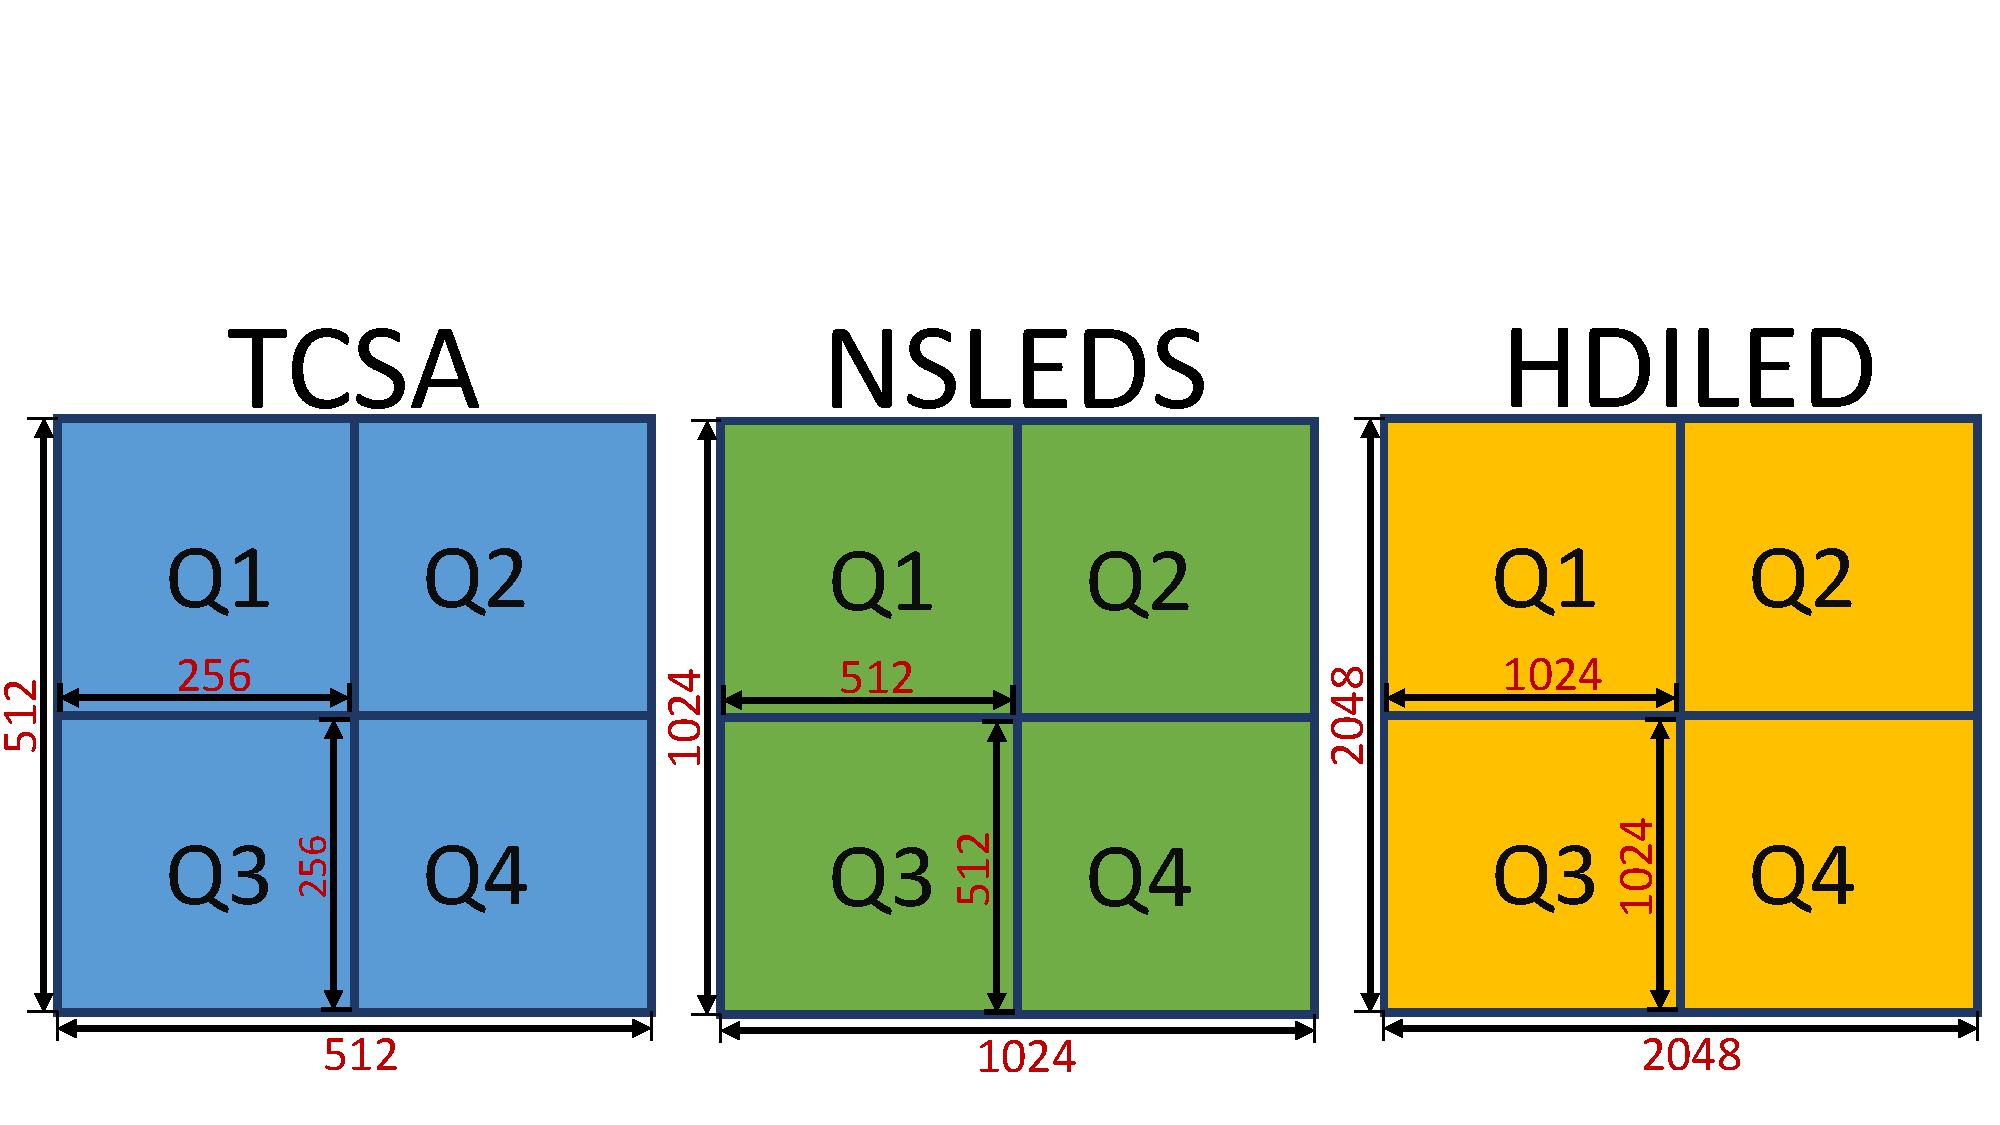
\includegraphics[width=1.0\textwidth]{fig/tcsa_nsleds_hdiled_quads.pdf}
        \caption[TCSA, NSLEDS, and HDILED Array Quadrant Layouts]{TCSA, NSLEDS, and HDILED Array Quadrant Layouts\textsuperscript{a}}
        \vspace{0px}
        \footnotesize\textsuperscript{a} Not drawn to scale
        \label{fig:tcsa_nsleds_hdiled_quads}
    \end{figure}

    The quadrant write enable selects which quadrant to drive. It is worth noting that each quadrant has separate internal signaling which allows for each quadrant to operate independently in parallel when mounted in a package that provides independent external signals as noted earlier. However, to date most of the fabricated IRLED arrays are mounted in packages that allows for only one quadrant to be drawn at a time. At the time of writing, only HDILED has been tested in the type of setup~\cite{LassiterEtAl2019_0, LassiterEtAl2019_1, LassiterEtAl2019_2, LassiterEtAl2020} due to it having the largest resolution per quadrant. During independent quadrant operation, multiple independent CSEs must be utilized. In a two CSE setup, half of the quadrant bits would be controlled by one CSE and half by another. This would yield a total of 64 channels being written in parallel for double the analog performance. In a four CSE setup, a single quadrant would be controlled by a single CSE. This would yield a total of 128 channels being written in parallel for quadruple the analog performance. Irrespective of the number of CSEs used to a drive an array, the internal RIIC signal lines would be driven in precisely the same manner within each quadrant with the only change being that they operate asynchronously with respect to the others.

    The X address, Y address, and LOAD are used to select which pixel or group of pixels to write within a quadrant depending on the mode of operation. Though these lines are effectively shared by quadrants in a single CSE Setup, within the RIIC architecture they can be driven independently to enable the multiple CSE operation mentioned previously. Internally, each array (or quadrants in multi-CSE setups) can write up to 32 pixels (or channels) of data at a given time. As noted previously, the mode of operation dictates whether 2, 4, 8, 16, or 32 channels are used. It also affects the number of address bits utilized in practice with lower modes of operation using more bits. Additionally, the number of address bits differs by array due to the differences in sizes. NSLEDS utilizes 7 bits for the X address and 7 bits for the Y address, yielding a total of 256 by 256 addresses per quadrant. The LOAD bit is used to select between even and odd rows, yielding an effective address space of 256 by 512 per quadrant. Because the smallest mode of operation writes 2 pixels at a time, this is sufficient to fully address the array. Similarly, HDILED utilizes 8 bits for the X address and 8 bits for the Y address, yielding a total of 512 by 512 addresses per quadrant. Again, as with NSLEDS, the LOAD bit is used to select between even and odd rows, yielding an effective address space of 512 by 1024 per quadrant. This is again sufficient to completely address the array since it also can at a minimize write 2 pixels at a time.

    Structurally, NSLEDS and HDILED are laid out as super pixel as shown in Figure~\ref{fig:nsleds_hdiled_array_superpixel_layout}. Each super pixel is made up of a grid of 4 pixels spanning two rows and columns. These are laid out across the array in a grid structure with NSLEDS consisting of 256 by 256 super pixels, and HDILED consisting of 512 by 512 super pixels. This image also highlights two points discussed above, the LOAD line selects between the top two pixels (even rows) and bottom two pixels (odd rows) of each super pixel in the quadrant, and the two selected pixels are both written at the same time. Additionally, these share a drive strength as noted in the diagram. This is controlled using the Strong/Weak drive strength bits which dictate whether to provide a strong or weaker light emission for the given pair of pixels.

    \begin{figure}
        \centering
        %includegraphs[trim=L B R T]
        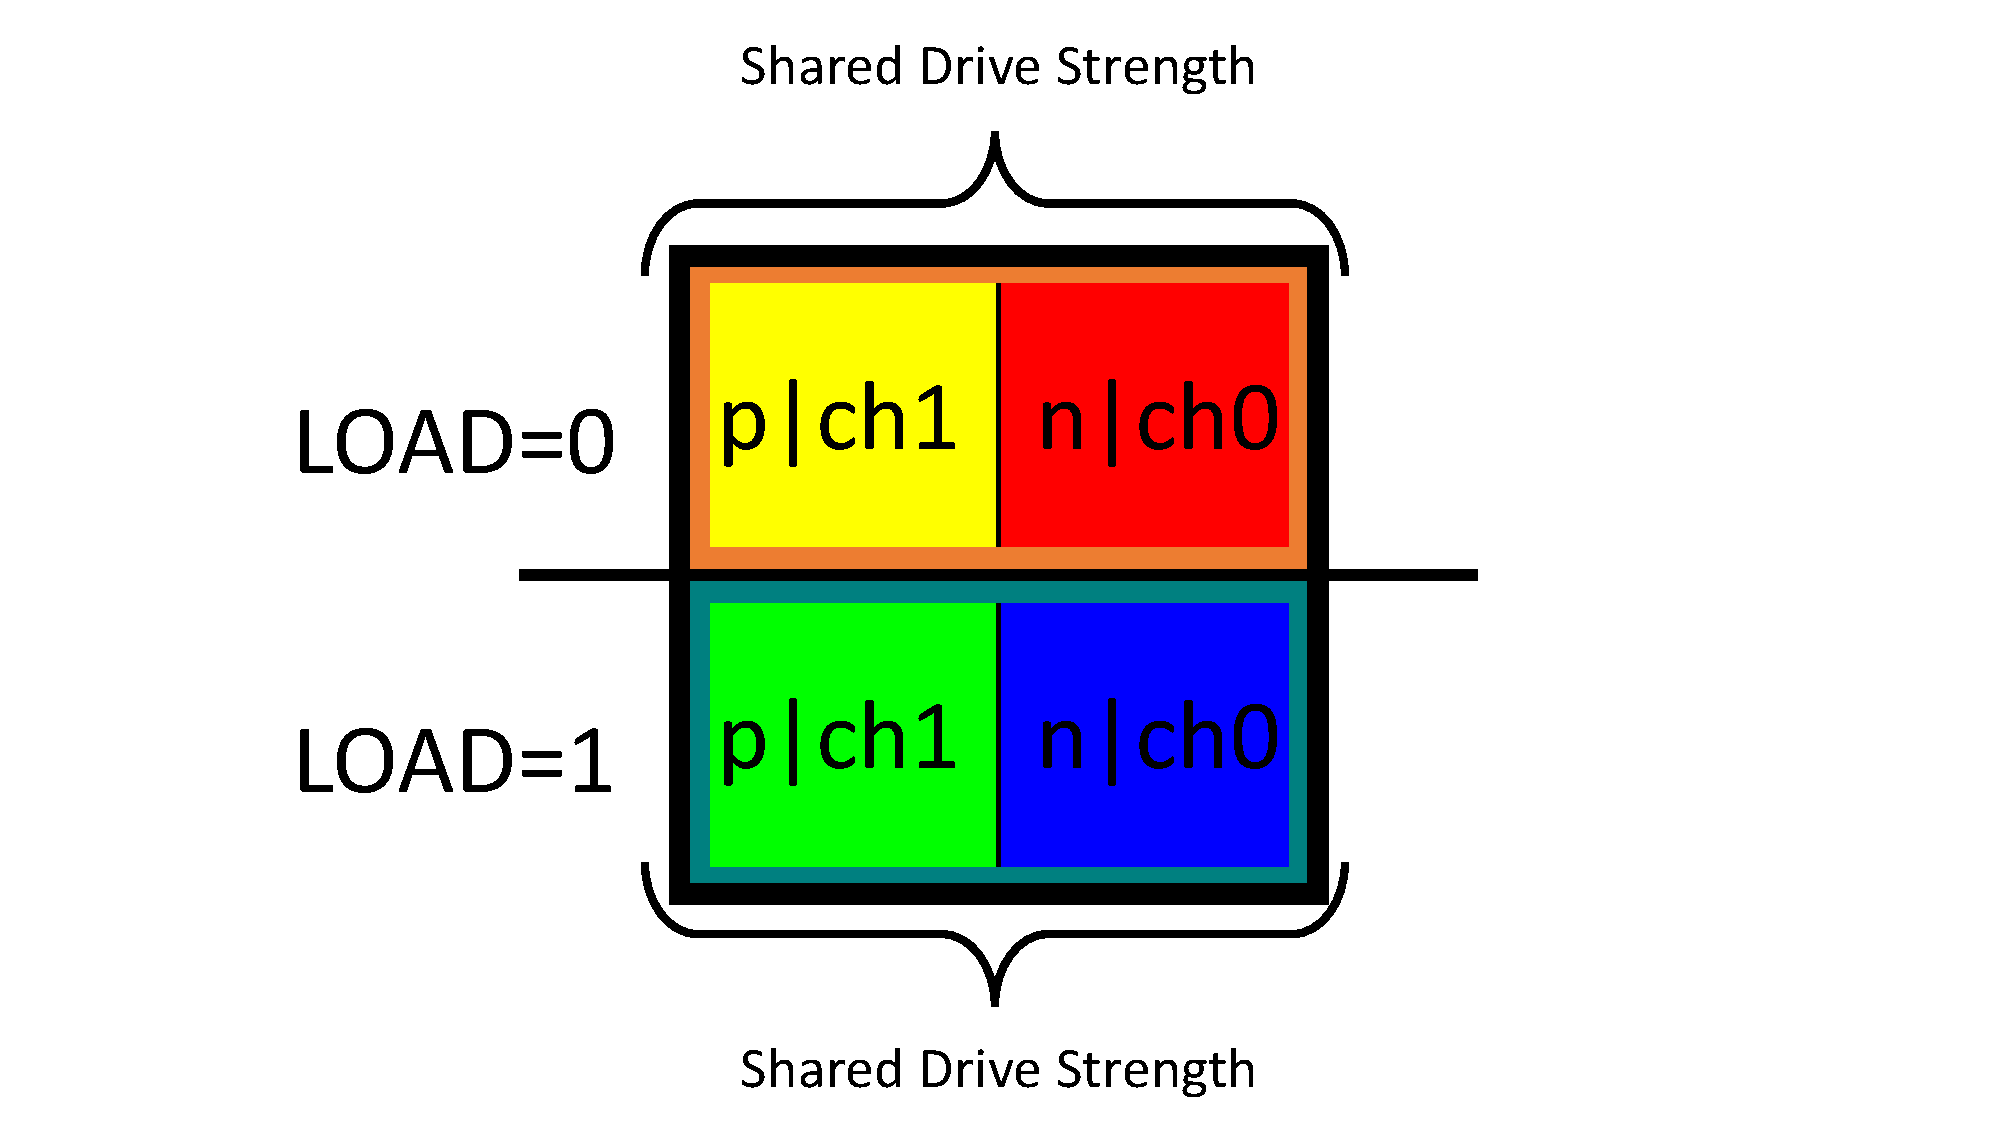
\includegraphics[width=0.50\textwidth]{fig/superpixel_layout.pdf}
        \caption{NSLEDS/HDILED Array Super Pixel Layout}
        \label{fig:nsleds_hdiled_array_superpixel_layout}
    \end{figure}

    The 32 analog signaling lines control the emission intensity of driven pixels. These 32 channels are controlled by digital to analog converters within the CSE that are driven by the firmware. Internally, a CSE has 8 DAC cards with 2 DAC integrated circuits per card, with each DAC circuit consisting of 2 DAC channels as discussed in Chapter~\ref{sec:close_support_electronics}. Each channel is used to drive a single pixel, giving the ability to drive 32 pixels at once or some subset as mentioned previously.

    In practice, it is preferable to utilize all channels at once because this allows for more pixels to be driven in a shorter amount of time. Each of the lower modes of operation cut analog bandwidth in half each time the channel count is halved. Figure~\ref{fig:nsleds_hdiled_array_interleaved_pixel_mapping_per_write} shows the pixel mapping per write for 32 physical pixels on an array in the highest mode of operation. 2 by 32 columns of pixels are shown segmented into super pixels. The Y address denotes the 16 super pixels that are selected per address. If the {\it Y Address} is incremented by 1 then the next 16 rows of super pixels would be selected. The {\it X address} (not shown) selects the next column of super pixels. {\it DAC Card} denotes which DAC card drives the given super pixel. {\it L} denotes which value of LOAD will select which rows within each super pixel. When LOAD is low as shown in the middle segment, the top pixels of a superpixel are selected as indicated in cyan. When LOAD is high as shown in the right segment, the bottom pixels of a superpixel are selected.

    \begin{figure}
        \centering
        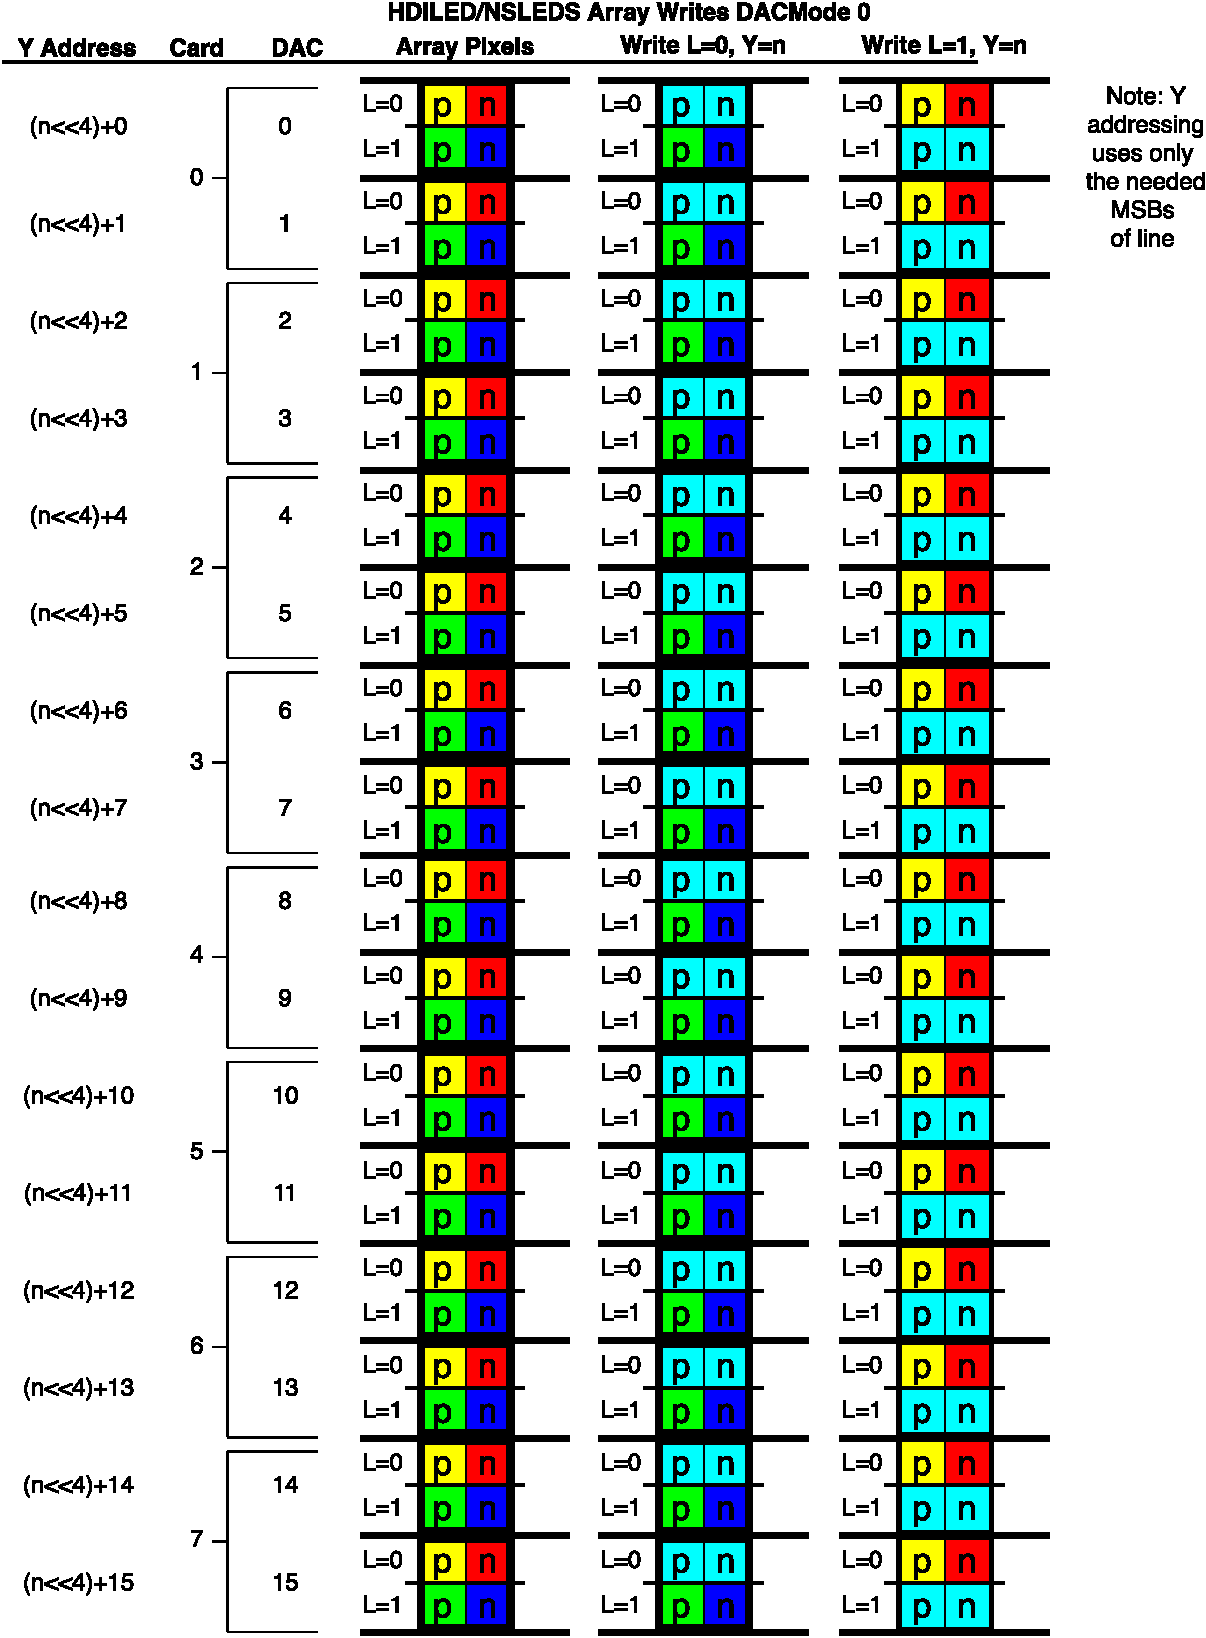
\includegraphics[width=0.98\textwidth]{fig/nsleds_hdiled_array_writing.pdf}
        \caption{NSLEDS/HDILED Array Interleaved Pixel Mapping Per Write}
        \label{fig:nsleds_hdiled_array_interleaved_pixel_mapping_per_write}
    \end{figure}

    The overall writing process for writing 64 pixels is a two-step process. First, 32 values for the even rows are loaded in and written to the array, followed by 32 values from the odd rows being loaded in and written to the array. At a data level, it is ideal to interleave the data such that it is available at the optimal time to reduce latency and buffering requirements within the firmware. This is discussed in detail in Chapter~\ref{chap:pdp_protocol}.

    Writing additional segments of pixels is a matter of buffering more data and repeating the same write process while asserting the correct address lines for each segment. Given that arrays have no inherit hardware required write order other than what has been discussed above, the exact order of writing independent segments of 32 pixels can change depending on a number of factors. In a single CSE Setup, under most circumstances, the data for the top quadrants is carried by a single HDMI input going into a CSE, and the data for the bottom quadrants carried by the other HDMI input\footnote{As will be discussed in Chapter~\ref{chap:implementation} when utilizing the PDP for driving an array, the location of where data is written to an array is agnostic to the HDMI input the data is transported on.}. In this case, the CSE firmware will swap between writing segments of 32 or 64 pixels to the top and bottom halves of an array. The former if it is desirable to write a minimal amount of data before servicing data from another input, the latter if it is desirable to complete an entire chunk of pixels. In a two CSE Setup, data over the HDMI links data could be segmented either horizontally or vertically meaning that each HDMI link would carry data for an entire quadrant. In a four CSE setup, each link would carry half of the data for a quadrant. As the reader may imagine, the order of writes could be configured in many different ways under these scenarios. Though it will not be discussed in detail within this dissertation, it is worth noting for posterity that the order of writes on IRLED arrays can and does affect the thermal load on an array which ultimately can effect pixel brightness~\cite{BarakhshanEtAl2017, LaVeigneSieglinger2012, Norton2013}; thus, controlling the order of writes can be an important factor to consider for designers and users of a system. As mentioned previously, many of these effects can be alleviated through a snapshot mode operation.

\section{Data ordering}
    \label{sec:data_ordering}
    Due to the interleaved write process described in Chapter~\ref{sec:array_Interleaved_write_process}, data sent to an array is reordered in a manner that simplifies firmware development and minimizes buffering requirements. Though the details of the PDP itself are discussed in later chapters, data ordering is discussed here to illustrate some performance considerations with array operation, and could be considered independent of the PDP in that the data ordering could be implemented in non-PDP firmware.

    Figure~\ref{fig:bit_packing} shows the data bit packing utilized within the system when the PDP is in use. It is designed to map to the superpixel layout shown in Figure~\ref{fig:nsleds_hdiled_array_superpixel_layout}. Shown is a 24-bit pixel word which normally represents an RGB value in RGB color space within display protocols where 8 bits are reserved for each of the red, green, and blue channels. Below this is the mapping of each bit value for an NSLEDS or HDILED array. Where {\it S} indicates the drive strength of the super pixel, {\it L} indicates the value to drive the left side of the super superpixel at, and {\it R} indicates the value to drive the right side of the superpixel at. Only 11 bits are currently used to transmit data per pixel due to bit resolution limitations in the DAC and amplifier boards used within a CSE. Future CSEs may have higher bit resolutions resulting in the need to transmit 16-bits per pixel. In this event bit packing would not be used. There has been some work on improving the DAC architecture as well~\cite{EjzakEtAl2019}.

    \begin{figure}
        \centering
        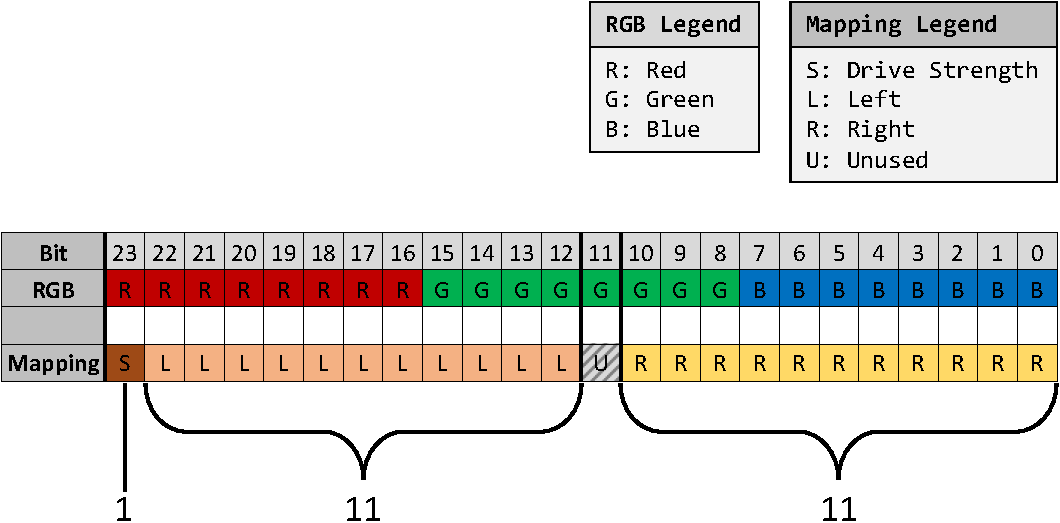
\includegraphics[width=1.0\textwidth]{fig/bit_packing.pdf}
        \caption{Bit-packing Format}
        \label{fig:bit_packing}
    \end{figure}

    Figure~\ref{fig:image_encoding} shows the input reordering performed on data sent to a CSE. Each cable sends half of the data as noted in Chapter~\ref{sec:close_support_electronics}. The input example is segmented into top, middle, and bottom to indicate which part goes over which input and the different reordering steps. The portions denoted as {\it Top} are transmitted over CSE input 1. The portions denoted as {\it Bottom} are transmitted over CSE input 2. The portions marked {\it Middle} are split evenly over both inputs evenly. The first step of data reordering is to bit pack into 11-bit words as shown in Figure~\ref{fig:bit_packing}. Next, even/odd reordering is performed to reduce latency and buffering constraints as will be shown in more detail in subsequent figures. Note the pattern introduced on the words in the diagram due to even/odd reordering. Finally, data is transposed before being sent to the array to accommodate the column write order of the array shown in Figure~\ref{fig:nsleds_hdiled_array_interleaved_pixel_mapping_per_write}. If data were not transposed, then multiple lines of data would need to be buffered to draw 32 pixels for a single write. In fact, the first generation of firmware utilized on the TCSA and NSLEDS arrays required full image buffering before displaying a single pixel on an array which resulted in an entire frame of latency during operation. The second generation of firmware~\cite{HouserEtAl2018} utilized on TCSA, NSLEDS, and HDILED drastically reduced buffering and latency requirements through data reordering, but
    required double the amount of buffering to that of the current implementation of the PDP because it did not have an even/odd row reorder step during encoding. This meant that 2 by 64 pixels of even and odd rows of data were required to be buffered before a single write could occur even though only 2 by 32 pixels are needed by the hardware for a single write. It is worth noting that as mentioned in Chapter~\ref{sec:array_Interleaved_write_process}, different arrays could have different rasterization processes, and in that event the transformations described here would need to be changed to minimize buffering for those scenarios.

    \begin{figure}
        \centering
        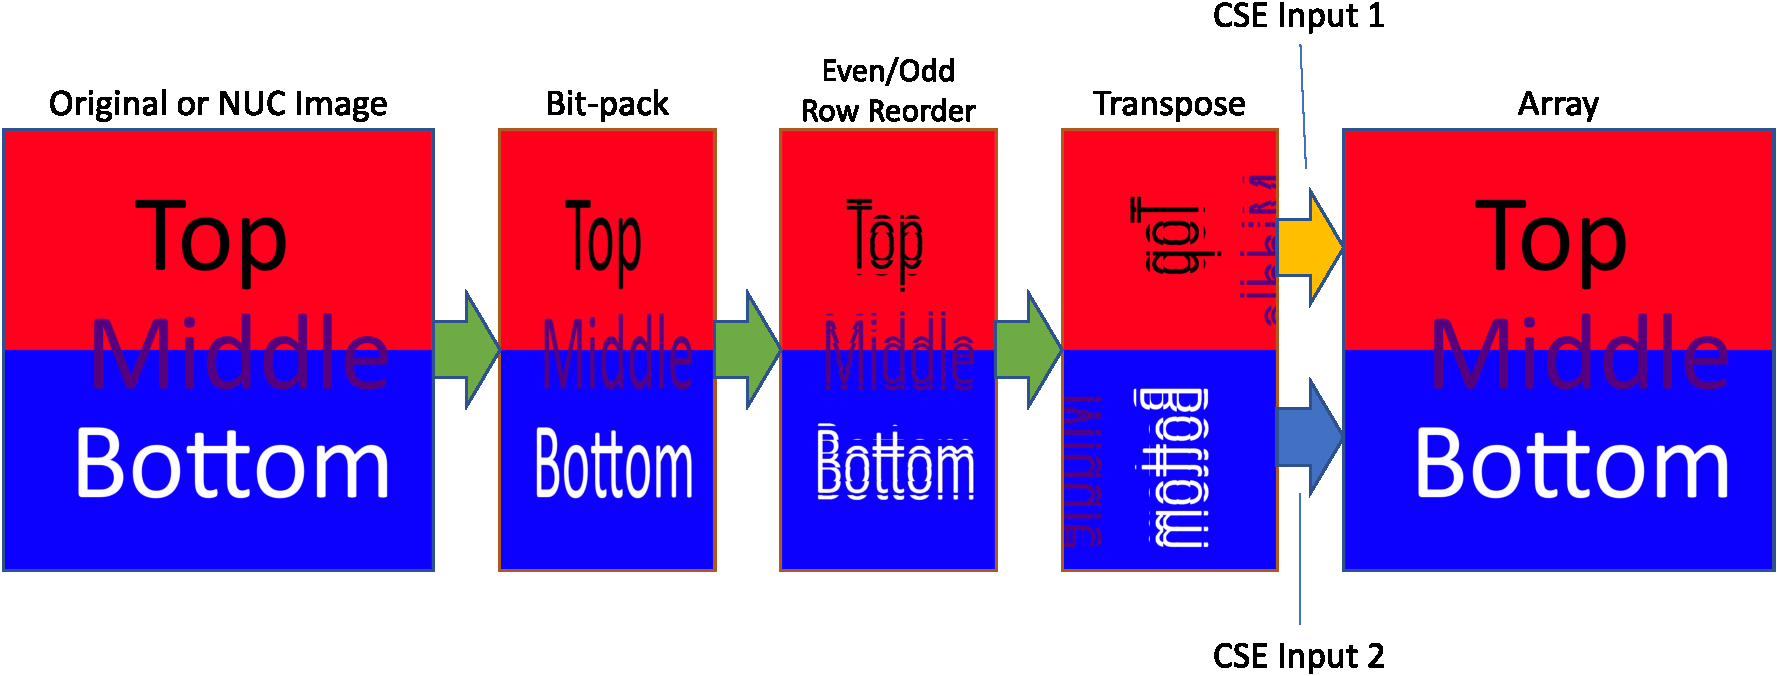
\includegraphics[width=1.0\textwidth]{fig/image_encoding.pdf}
        \caption{Image Encoding: Input Reordering}
        \label{fig:image_encoding}
    \end{figure}

    Figure~\ref{fig:image_encoding_quads} shows how the same image data maps to each quadrant on an array. Similarly, to the previous image the separation of top, middle, and bottom by input cable holds here. Additionally, shown is that quadrant one and two are transmitted over the first input and quadrant three and four over the second input. Note also that the top-left of the image corresponds to quadrant one, the top-right of the image corresponds to quadrant two, the bottom-left of the image corresponds to quadrant three, and the bottom-right of the image corresponds to quadrant four. This relationship holds for all subsequent images. Figure~\ref{fig:image_encoding_colored} shows the same details in a color overlayed chart.

    \begin{figure}
        \centering
        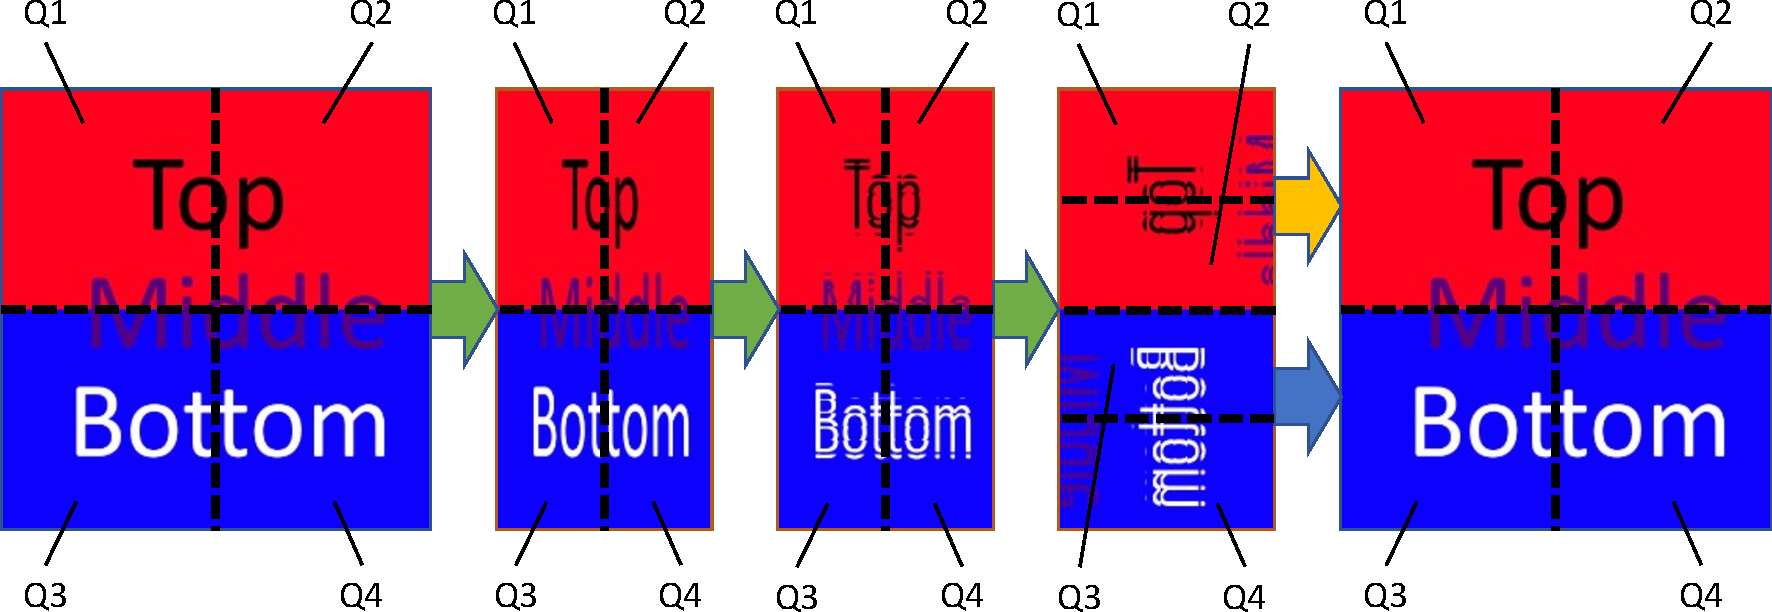
\includegraphics[width=1.0\textwidth]{fig/image_encoding_quads.pdf}
        \caption{Image Encoding: Quadrant Reordering}
        \label{fig:image_encoding_quads}
    \end{figure}

    \begin{figure}
        \centering
        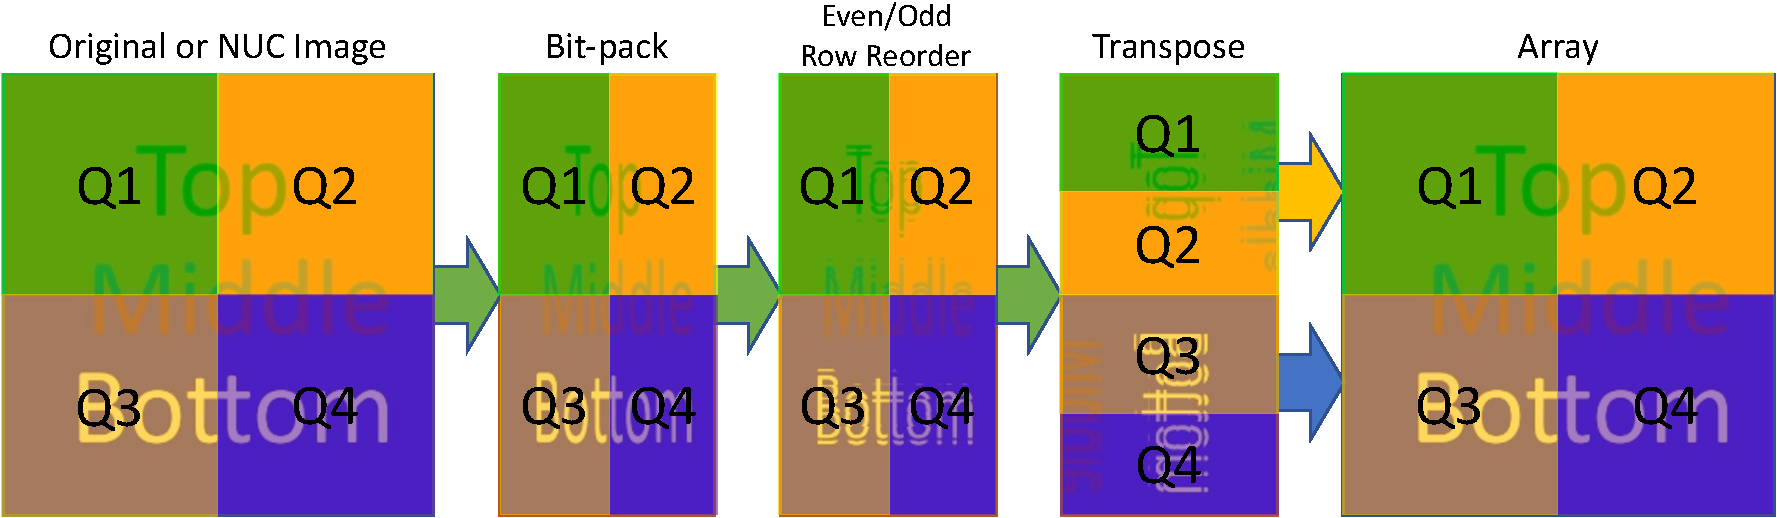
\includegraphics[width=1.0\textwidth]{fig/image_encoding_colored.pdf}
        \caption{Image Encoding: Quadrant Reordering with Color Overlay}
        \label{fig:image_encoding_colored}
    \end{figure}

    Figure~\ref{fig:image_encoding_bitback} shows the bit-packing process for a false color image to aid with understanding. The blown-up sections show single columns of data and the corresponding bit packed version of the data where two columns of input with different colors of data per column are merged into a single column of 24-bit data with one color. This results in the example input image having two solid colors after bit-packing. In the actual implementation of bit packing, real data is in the IR-spectrum and not averaged in this way but clamped and scaled instead. While not required, generally IR data is normally 16-bits per pixel which corresponds to current higher-class IR detectors having a dynamic range of 14-bits per pixel~\cite{FLIR2014_1, FLIR2014_2, FLIR2016}. Cheaper detectors may only have lower dynamic ranges resulting in a lower ability to differentiate light output. Even/odd reordering and the transpose do not result in any noticeable data changes for this example.

    \begin{figure}
        \centering
        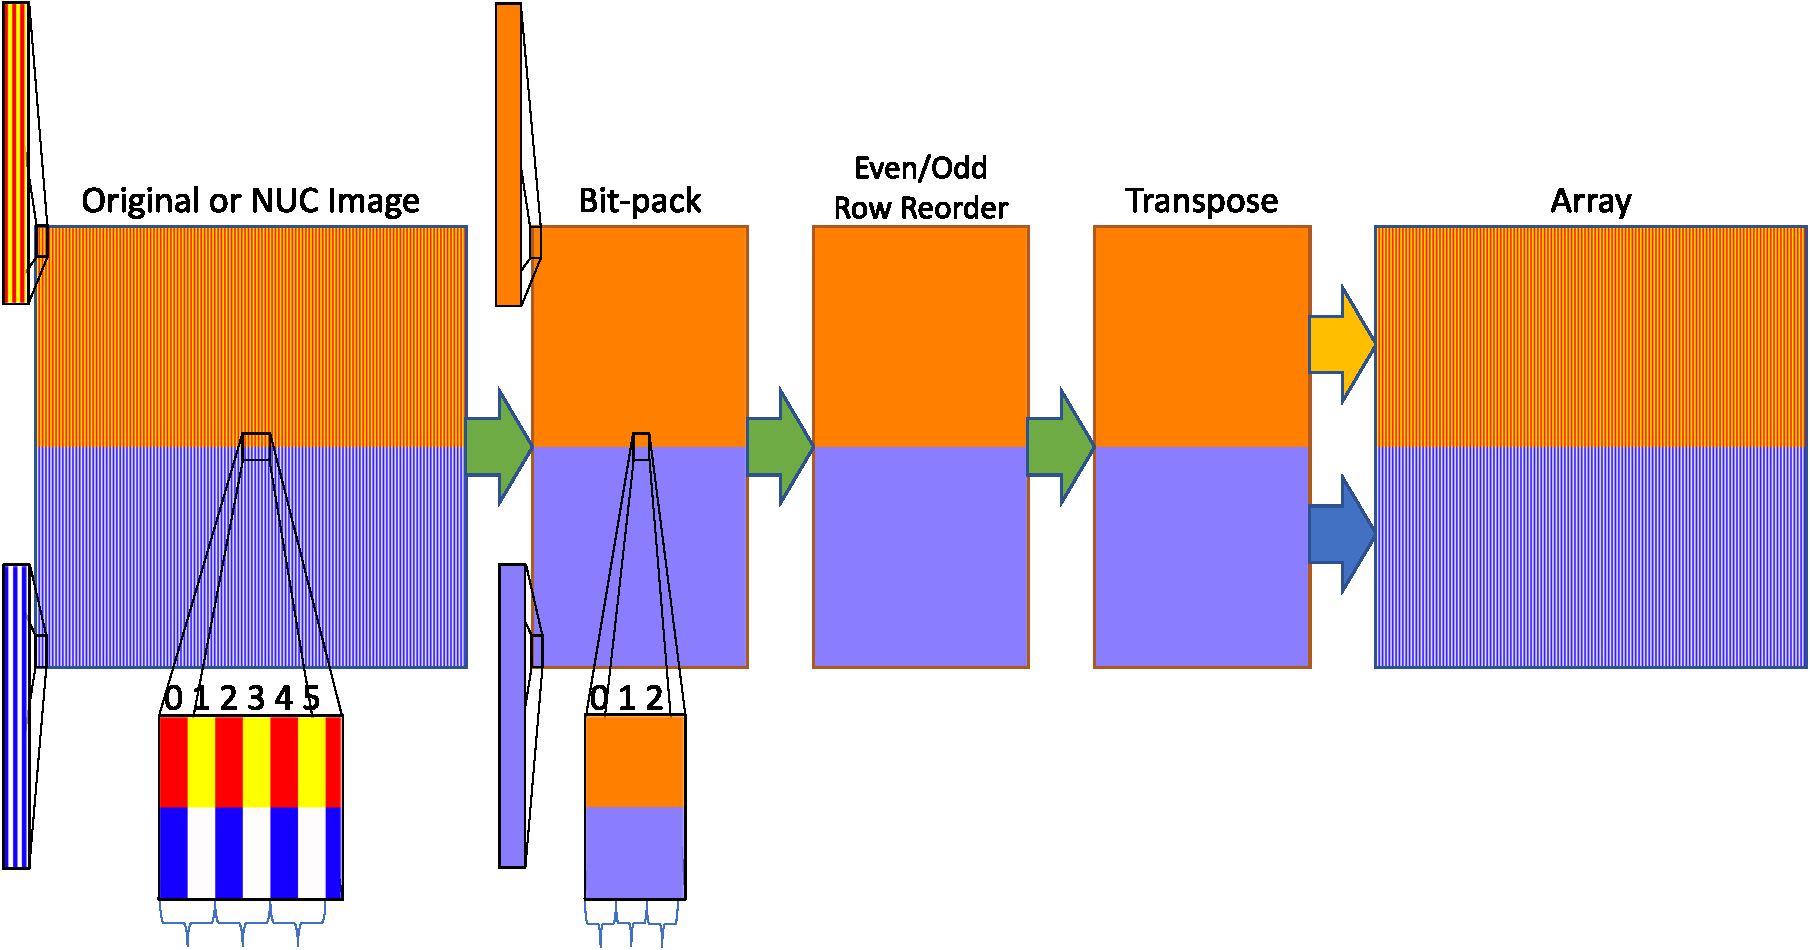
\includegraphics[width=1.0\textwidth]{fig/image_encoding_bitback.pdf}
        \caption{Image Encoding: Data Bit Packing}
        \label{fig:image_encoding_bitback}
    \end{figure}

    Figure~\ref{fig:image_encoding_bitpack_reorder} shows a false color input image designed to highlight the even/odd row reordering applied to imagery. The blown-up sections show 64 labeled rows of input data where the even rows are one color and the odd rows another color for every 32 rows. Additionally, for every 32 rows, the even and odd rows are de-interlaced into 16 even rows of data follow by 16 odd rows of data. In the example input image this results in every 16 de-interlaced rows having a different color. This is due to the interleaved write process for individual 32-pixel writes discussed in Chapter~\ref{sec:array_Interleaved_write_process}. Reordering data allows for only 16 bit-packed pixels of data to be buffered per write. As discussed previously, without this reordering, double the number of pixels would need to be buffered per array write increasing both latency and implementation complexity.

    \begin{figure}
        \centering
        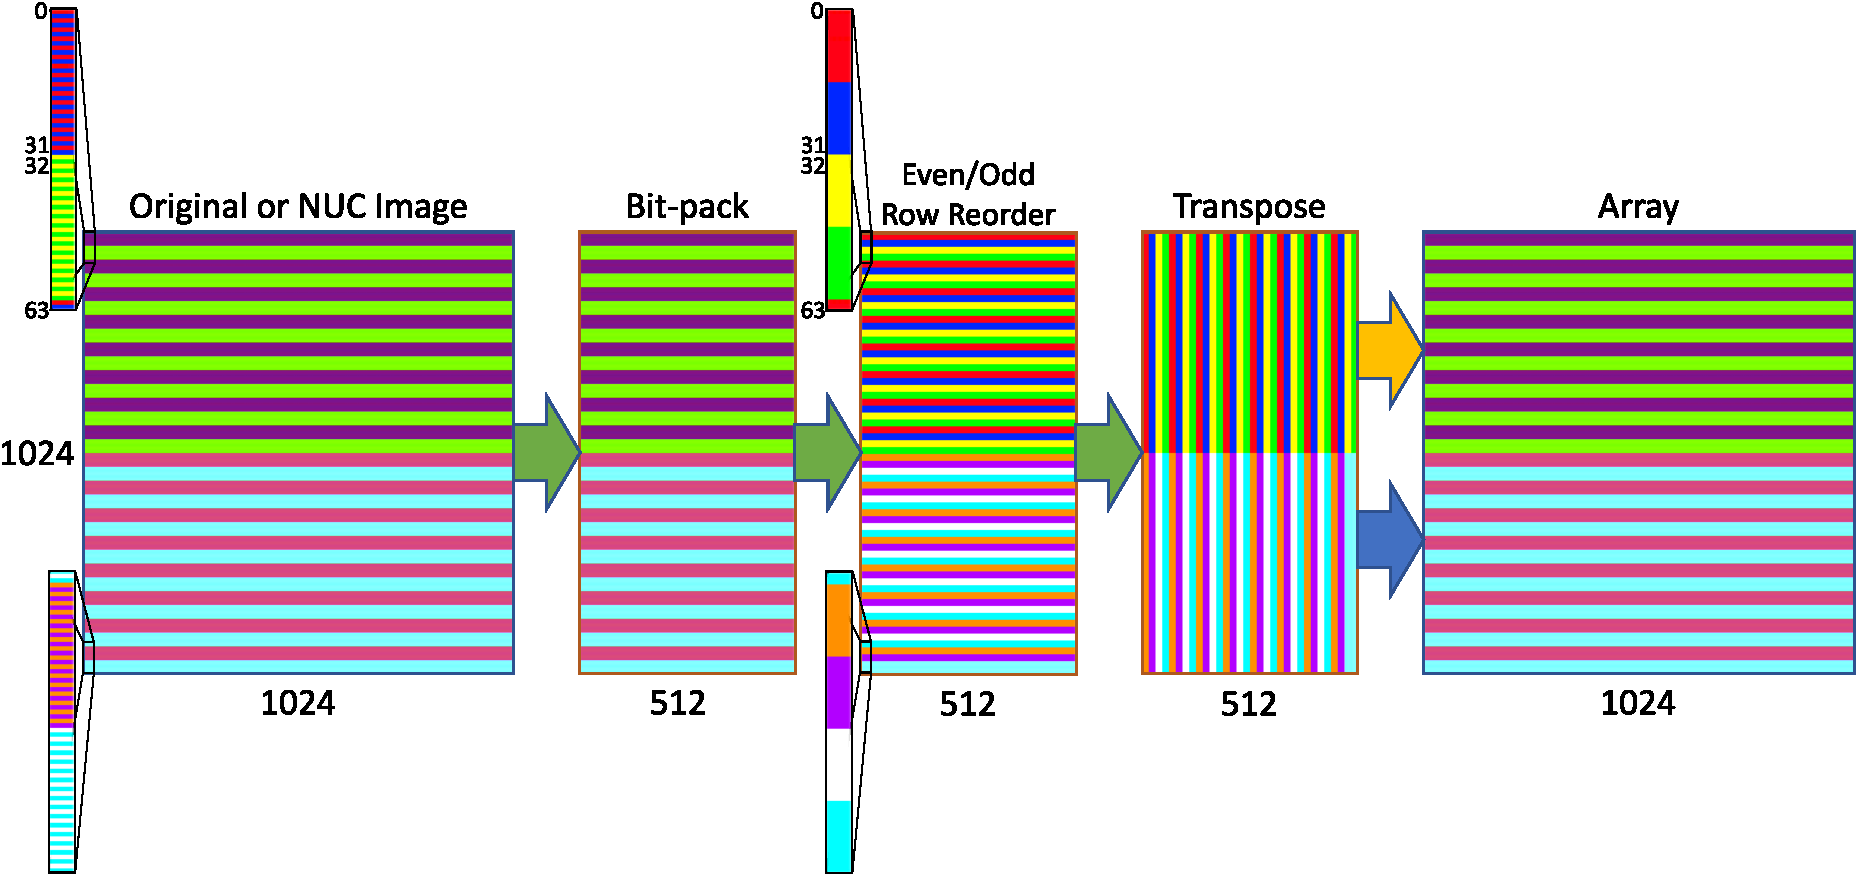
\includegraphics[width=1.0\textwidth]{fig/image_encoding_reorder.pdf}
        \caption{Image Encoding: Data Reorder}
        \label{fig:image_encoding_bitpack_reorder}
    \end{figure}

    Figures~\ref{fig:image_encoding_color_example1},~\ref{fig:image_encoding_color_example2},~and~\ref{fig:image_encoding_color_example3} show some examples of what false colored images would look like if processed by the reordering kernels to give the reader a better understanding of how different types of data would look during the intermediate processes. Note the characteristic jagged pattern due to even/odd row reordering present in each image. Also note that each image is transposed and segmented in half for transfer over separate inputs to a CSE.

    \begin{figure}
        \centering
        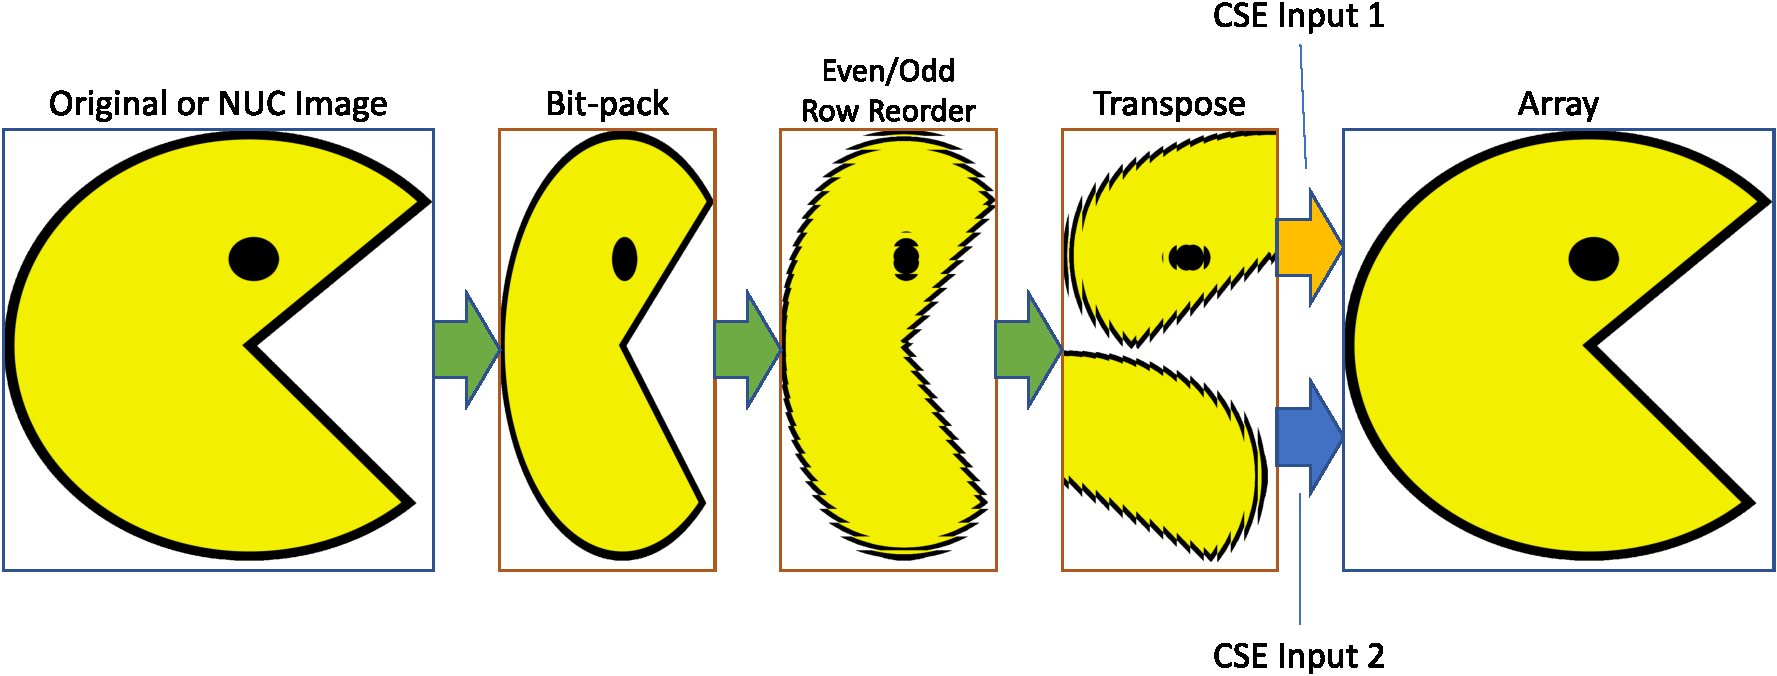
\includegraphics[width=1.0\textwidth]{fig/image_encoding_pac.pdf}
        \caption{Image Encoding: Color Example 1}
        \label{fig:image_encoding_color_example1}
    \end{figure}

    \begin{figure}
        \centering
        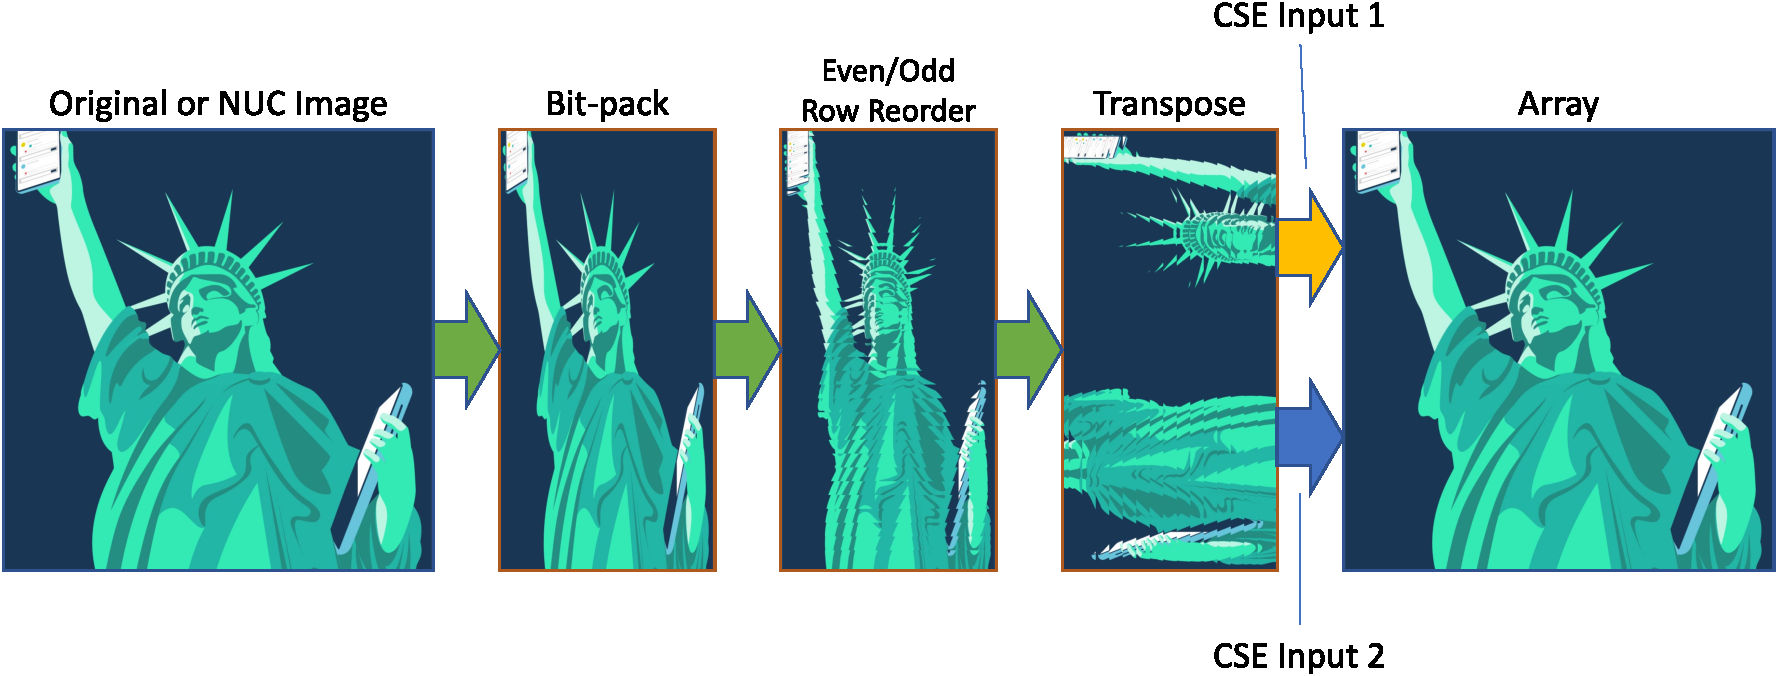
\includegraphics[width=1.0\textwidth]{fig/image_encoding_liberty.pdf}
        \caption{Image Encoding: Color Example 2}
        \label{fig:image_encoding_color_example2}
    \end{figure}

    \begin{figure}
        \centering
        %includegraphs[trim=L B R T]
        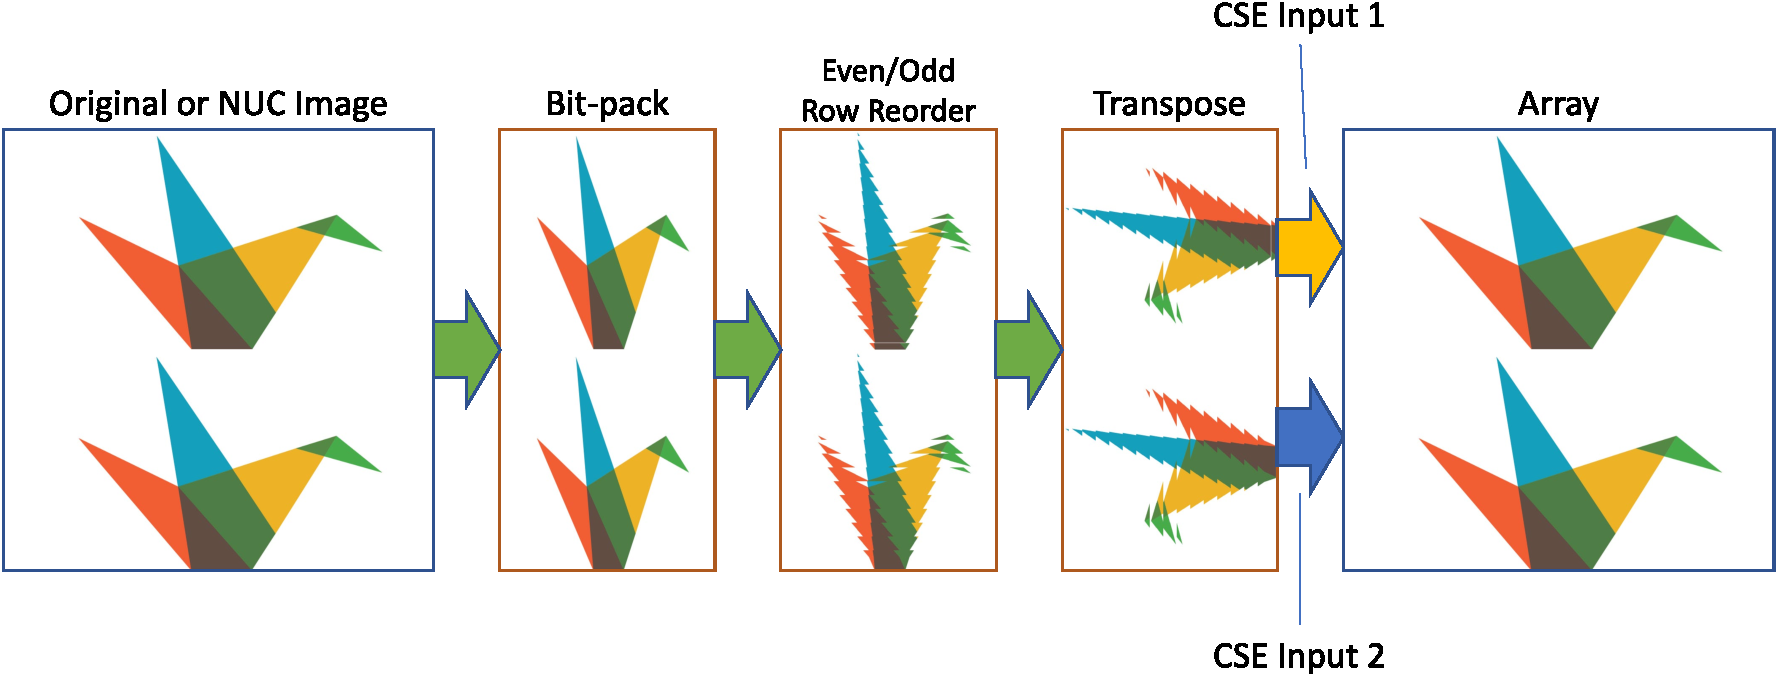
\includegraphics[width=1.0\textwidth]{fig/image_encoding_origami.pdf}
        \caption{Image Encoding: Color Example 3}
        \label{fig:image_encoding_color_example3}
    \end{figure}

    Figures~\ref{fig:image_encoding_ir_example1},~and~\ref{fig:image_encoding_ir_example2} show IR imagery going through the process of reordering. The image shown in Figure~\ref{fig:image_encoding_ir_example1} is commonly used to focus IR cameras and for testing IR array behavior with various shapes and numbers. The image shown in Figure~\ref{fig:image_encoding_ir_example2} is test imagery from one of the projects of my lab. Similarly, to the false color images, images are transposed and sent in halves over the CSE inputs.

    \begin{figure}
        \centering
        %includegraphs[trim=L B R T]
        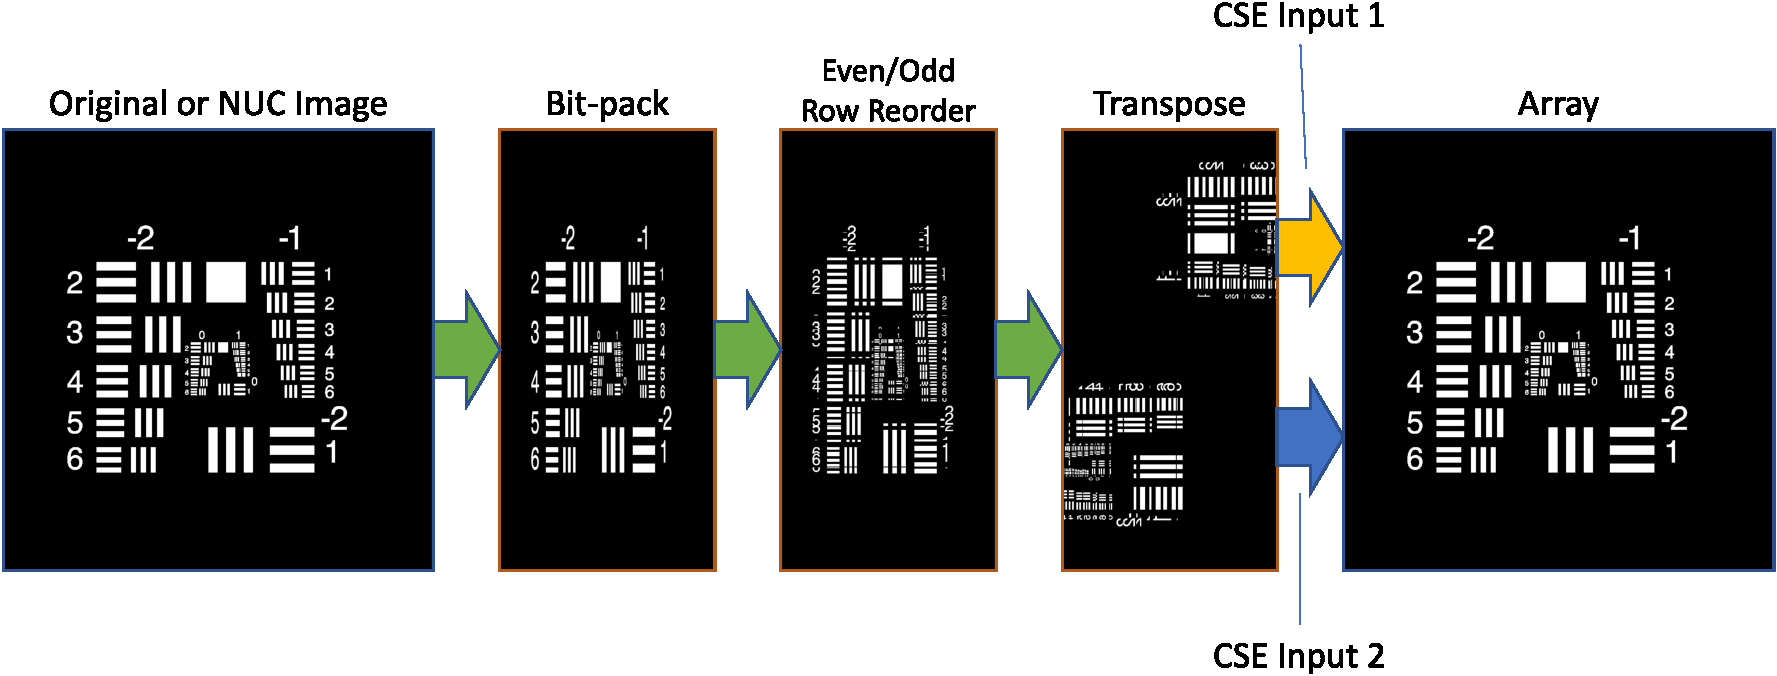
\includegraphics[width=1.0\textwidth]{fig/image_encoding_ir1.pdf}
        \caption{Image Encoding: IR Example 1}
        \label{fig:image_encoding_ir_example1}
    \end{figure}

    \begin{figure}
        \centering
        %includegraphs[trim=L B R T]
        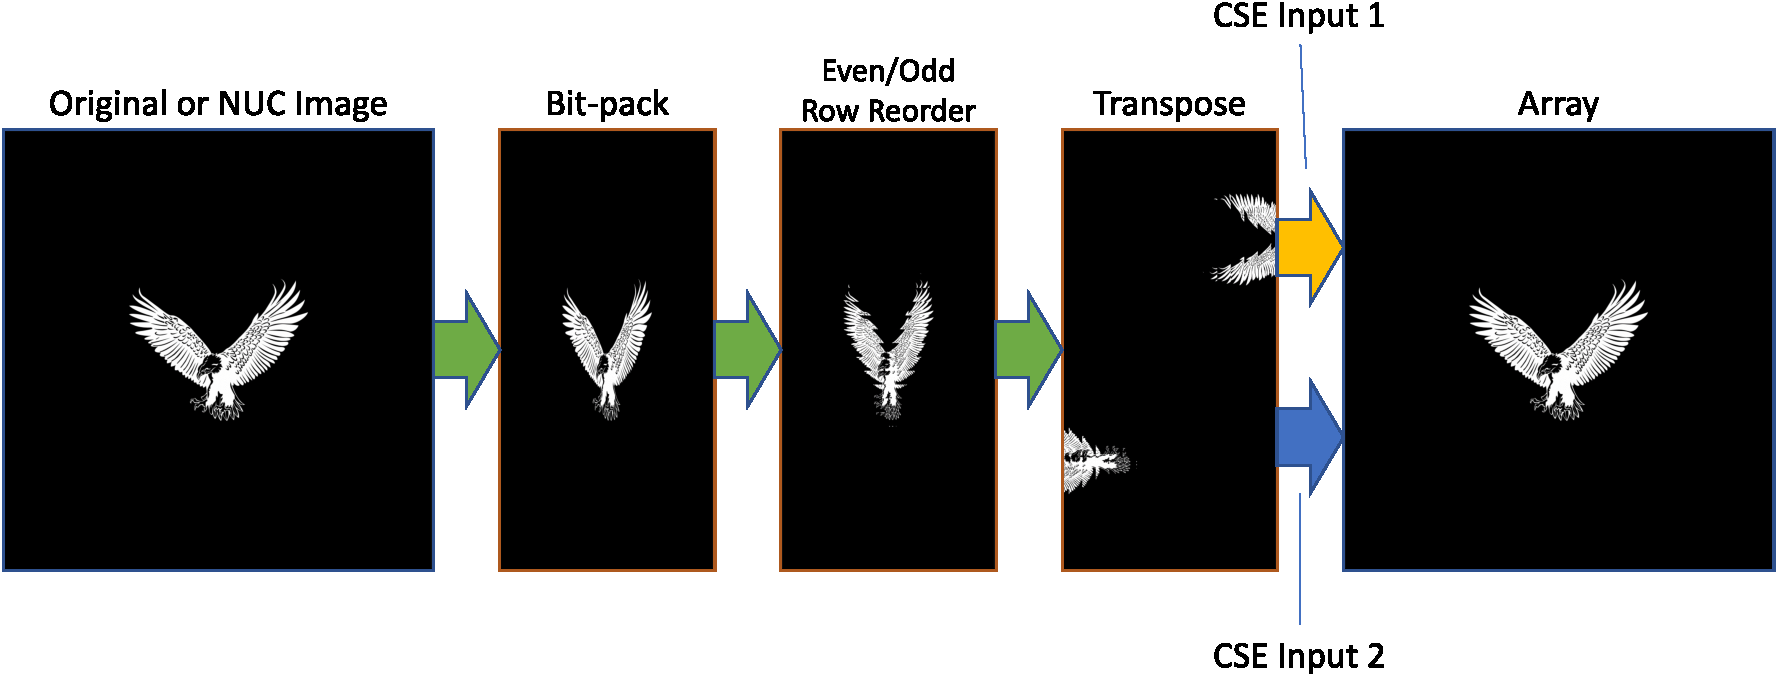
\includegraphics[width=1.0\textwidth]{fig/image_encoding_ir2.pdf}
        \caption{Image Encoding: IR Example 2}
        \label{fig:image_encoding_ir_example2}
    \end{figure}

    While this chapter discussed the internal details of how imagery received within the array is formatted and written to an array, Chapter~\ref{chap:display_protocols} shifts to a discussion of how imagery is sent to an array at the protocol level within an IRSP system while providing details of the limitations and challenges present there.

    \chapter{Display Protocols} % DONE
        \label{chap:display_protocols}
This chapter discusses the details of display protocols. Firstly, it provides a general discussion of how common display protocols work to send pixel data to a display system (e.g. a television). Then, it discusses how these protocols are utilized within IRSP technology.

\section{Conventional Display Protocols}
    \label{sec:conventional_display_protocols}

    Display specifications such as DSI~\cite{HDMIForum2017}, DVI~\cite{DDWG1999}, HDMI~\cite{HDMIForum2018}, and DisplayPort~\cite{VESA2016} are the backbone of consumer electronic display devices\footnote{Some newer additions such as Variable Refresh Rate (VRR) and the framing of DisplayPort are discussed in Chapter~\ref{chap:pdp_protocol} to allow for a direct comparison with the PDP.} They are utilized in a plethora of devices ranging from televisions, monitors, laptops, smart phones, to embedded devices such as point of sale (POS) terminals. Increasingly, they are being utilized in the ever-increasing smart display market for applications such as registration, product menus, smart watches, etc.

    These generally provide a standardized feature-set, or display protocol, that is rooted in classical analog video specifications (e.g. VGA, Composite)~\cite{NI2018} that utilize scan lines~\cite{Neal1998}. Scan lines are used to provide video timing information to synchronize a display to a given refresh rate. Each scan line consists of an active video region followed by a horizontal blanking period. After all active video scan lines are displayed, a vertical synchronization region is used to indicate the end of a frame.

    An overview of this is shown in Figure~\ref{fig:display_protocol_timing_overview}. The region shown in green is the pixel data for the active video region of the display. It is of size $h_a\cdot v_a$ which represents the number of pixels to display, for example, 1920 by 1080 for a HDTV high-definition video mode~\cite{MythTV2015}. The blanking time regions denote pixel data that is sent but not displayed\footnote{Typically data lines are held low during this period, but sometimes they are used for out-of-band communication to send other information such as audio encoding.}. A scan line consists of pixels made up of the $h_a+h_{fp}+h_{sp}+h_{bp}$ regions. These are the horizontal active size, the horizontal front porch, the horizontal sync pulse, and the horizontal back porch, respectively. $v_a$, the vertical active size, indicates the number of scanlines that make up the active region of the display. The vertical blanking period makes up multiple scanlines and consists of $v_{fp}+v_{sp}+v_{bp}$ scanlines. These are the vertical front porch before the vsync pulse, the vertical sync pulse, and the vertical back porch, respectively. Sync pulses are generally active low, meaning that during active display a sync signal is high as shown in the diagram. Note, that this terminology is consistent with the VESA Coordinated Video Timings (CVT) Standard~\cite{VESA2013}.

    Figure~\ref{fig:display_protocol_line_cross} shows a closeup view of signal lines during the active region of display for two scan lines\footnote{The active pixel count is proportionally smaller to blanking regions than in real modes for illustration purposes.}. A data enable signal denoted by $enable$ is high during the active region shown in green. Following this, it goes low for a period of time denoted by the $h_{fp}+h_{sp}+h_{bp}$ regions. The horizontal sync signal goes low only in the region shown in yellow between the front porch and back porches. This process repeats for all scan lines. Once the last active region pixel is drawn, the enable signal will stop going high during the vertical synchronization period.

    Figure~\ref{fig:display_protocol_full_cross} shows a closeup view of signal lines during the transition into the vertical synchronization period\footnote{The blanking regions consist of less scanlines than in real modes for illustration purposes.}. The region donated by $v_a$ indicates the end of the video active region of the display which occurs toward the end of a frame. After the active video region, all data has been drawn to a display. The region denoted by $v_{fp}+v_{sp}+v_{bp}$ is the vertical blanking or vsync period during which no active video data is sent; therefore, data enable denoted by $enable$ is always low during this period. Before the vertical sync pulse period denoted by $v_{sp}$ occurs, a vertical front porch period denoted by $v_{fp}$ occurs. After the vertical sync pulse, a vertical back porch region $v_{bp}$ occurs. Following this, the beginning of the next frame begins after the $v_{bp}$ region.

    \begin{figure}[H]
        \centering
        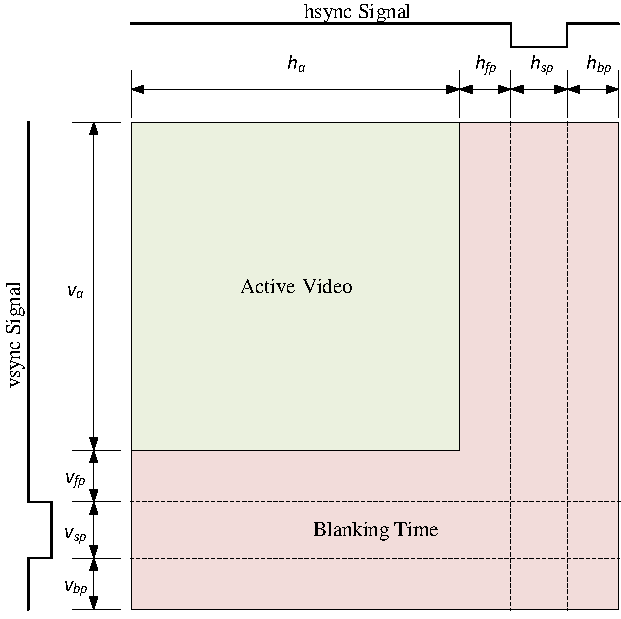
\includegraphics[width=1.0\textwidth]{fig/display_timing_overview.pdf}
        \caption{Display Protocol Timing Overview}
        \label{fig:display_protocol_timing_overview}
    \end{figure}

    \begin{figure}[H]
        \centering
        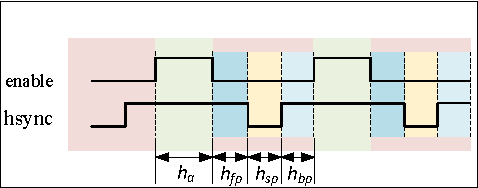
\includegraphics[width=1.0\textwidth]{fig/display_timing_line_cross.pdf}
        \caption{Display Protocol Horizontal Signal Cross Section Timing}
        \label{fig:display_protocol_line_cross}
    \end{figure}

    \begin{figure}[H]
        \centering
        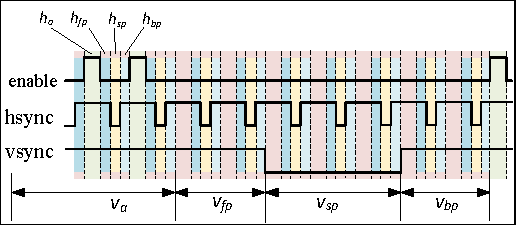
\includegraphics[width=1.0\textwidth]{fig/display_timing_full_cross.pdf}
        \caption{Display Protocol Full Signal Cross Section Timing}
        \label{fig:display_protocol_full_cross}
    \end{figure}

    Equations~\eqref{eq:l_h}~through~\eqref{eq:f_t} show the relationship between the different regions of a display and the frequency or refresh rate. In Equation~\eqref{eq:l_h}, $l_h$ denotes the scan line size of a display, or total horizontal width, which is made up of the horizontal active and horizontal porch region pixels of a display. In Equation~\eqref{eq:l_v}, $l_v$ denotes the total vertical width of a display, which is made up the vertical active and vertical porch region pixels of a display. In Equation~\eqref{eq:f_f}, each pixel is sent at a rate denoted by $f_p$, the pixel frequency (also called the pixel clock) where the result $f_f$ denotes the frame frequency or frame rate of a display. This is simply the pixel frequency over the total number of pixels (video active and porches) of a display. In Equation~\eqref{eq:p_t}, $p_t$ denotes the time period a single pixel takes to send. In equation~\eqref{eq:f_t}, $f_t$ denotes the time period for an entire frame.


    \begin{equation}
        l_h=h_a+h_{fp}+h_{sp}+h_{bp}
        \label{eq:l_h}
    \end{equation}
    \begin{equation}
        l_v=v_a+v_{fp}+v_{sp}+v_{bp}
        \label{eq:l_v}
    \end{equation}
    \begin{equation}
        f_f={\frac{f_p}{l_h \cdot l_v}}
        \label{eq:f_f}
    \end{equation}
    \begin{equation}
        p_t={\frac{1}{f_p}}
        \label{eq:p_t}
    \end{equation}
    \begin{equation}
        f_t={\frac{1}{f_f}}
        \label{eq:f_t}
    \end{equation}

    To illustrate, let us look at the display modeline generated using the VESA Coordinated Video Timing (CVT) standard shown in Table~\ref{tbl:modeline_example}. This modeline operates a total frame frequency of approximately \mbox{30 Hz}. The pixel clock 79.75, denoted in red, is specified in megahertz. The horizontal pixels, denoted in blue; are the horizontal display width, the horizontal sync start, the horizontal sync end, and the horizontal total pixels, respectively. The vertical pixels (measured in lines), denoted in green; are the vertical display height, the vertical sync start, the end of vertical sync end, and the horizontal total pixels, respectively. The sync pulse polarities, denoted in yellow; indicate whether a given sync pulse is active low or active high. A minus symbol indicates active low and a plus symbol indicates active high. The terminology for these modeline parameters comes from The X Window System~\cite{TheOpenGroup2020}, a commonly utilized windowing system in the Linux family of operating systems where the parameters, while equivalent, are specified in a different format from the VESA standards. Equations~\eqref{eq:h_a_solve}~and~\eqref{eq:v_a_solve} show the relationship between the X Window System parameters and the VESA parameters.

    \begin{table}
        \small
        \setlength\tabcolsep{2pt}
        \begin{tabular}{| c c c c c |}
            \hline
                \textbf{\footnotesize Name} & \begin{tabular}{c} \textbf{\footnotesize Pixel} \\ \textbf{\footnotesize Clock} \\ \textbf{\footnotesize (MHz)} \end{tabular}
                & \begin{tabular}{c} \textbf{\footnotesize Horizontal} \\ \textbf{\footnotesize Parameters} \\ \textbf{\footnotesize (pixels)} \end{tabular}
                & \begin{tabular}{c} \textbf{\footnotesize Vertical} \\ \textbf{\footnotesize Parameters} \\ \textbf{\footnotesize (lines)} \end{tabular}
                & \textbf{\footnotesize Polarity} \\ \hline
                & $f_p$ & $h_D \quad h_{SS} \quad h_{SE} \quad h_{T}$ & $v_D \quad v_{SS} \quad v_{SE} \quad v_{T}$ &
                \\
                \textbf{``1920x1080\_30.00"} & {\color{red}79.75} & {\color{blue} 1920 1976 2168 2416} &  {\color{darkgreen}1080 1083 1088 1102} & {\color{olive}-hsync +vsync} \\
            \hline
        \end{tabular}
        \caption{Bandwidth requirements of a conventional display protocol}
        \label{tbl:modeline_example}
        %\end{small}
    \end{table}

    \begin{equation}
        \begin{array}{ l l l l }
            \displaystyle
            h_a=h_D & h_{fp}=h_{SS}-h_a & h_{sp}=h_{SE}-h_{SS} & h_{bp}=h_T-h_{SE} \\
            h_a=1920 & h_{fp}=1976-1920 & h_{sp}=2168-1976 & h_{bp}=2416-2168 \\
            h_a=1920 & h_{fp}=56 & h_{sp}=192 & h_{bp}=248
        \end{array}
        \label{eq:h_a_solve}
    \end{equation}

    \begin{equation}
        \begin{array}{ l l l l }
            \displaystyle
            v_a=v_D & v_{fp}=v_{SS}-v_a & v_{sp}=v_{SE}-v_{SS} & v_{bp}=v_T-v_{SE} \\
            v_a=1080 & v_{fp}=1083-1080 & v_{sp}=1088-1083 & v_{bp}=1102-1088 \\
            v_a=1080 & v_{fp}=3 & v_{sp}=5 & v_{bp}=14
        \end{array}
        \label{eq:v_a_solve}
    \end{equation}

    If the parameters for the modeline in Table~\ref{tbl:modeline_example} are placed into the formulas shown in Equations~\eqref{eq:l_h} through \eqref{eq:f_t}, the results shown in Equations~\eqref{eq:l_h_solve} through \eqref{eq:f_t_solve} are yielded. The astute reader will note that $l_h$ and $l_v$ are the same as the total width and height for the given modeline. The pixel period is $\sim12.53 ns$, meaning that each pixel is drawn for the given amount of time. The frame period is $\sim33.38 ms$, meaning that each frame is drawn for that given amount of time.

    \begin{equation}
        \begin{array}{ l }
            \displaystyle l_h=h_T=h_a+h_{fp}+h_{sp}+h_{bp} \\
            \displaystyle l_h=h_T=1920+56+192+248 \\
            \displaystyle l_h=h_T=2416
            \label{eq:l_h_solve}
        \end{array}
    \end{equation}

    \begin{equation}
        \begin{array}{ l }
            \displaystyle l_v=v_T=v_a+v_{fp}+v_{sp}+v_{bp} \\
            \displaystyle l_v=v_T=1080+3+5+14 \\
            \displaystyle l_v=v_T=1102 \\[11pt]
        \end{array}
        \label{eq:l_v_solve}
    \end{equation}

    \begin{equation}
        \begin{array}{ l }
            \displaystyle f_f={\frac{f_p}{l_h \cdot l_v}} \\[11pt]
            \displaystyle f_f={\frac{79.75e^6}{2416 \cdot 1102}} \\[11pt]
            \displaystyle f_f={29.95} \\[11pt]
        \end{array}
        \label{eq:f_f_solve}
    \end{equation}

    \begin{equation}
        p_t=12.53ns={\frac{1}{f_p}}
        \label{eq:p_t_solve}
    \end{equation}

    \begin{equation}
        f_t=33.38ms={\frac{1}{f_f}}
        \label{eq:f_t_solve}
    \end{equation}

\section{Display Protocols within IRSP Technology}
    \label{sec:displays_within_proj_system}
    IRSP technology typically utilizes conventional display protocol technology to drive IR-arrays. In the most basic form a scene generator will provide imagery that is encoded utilizing a display protocol and send it to some form of close support electronics which will then decode the stream pixel by pixel and drive an array as discussed in Chapter~\ref{chap:array_write_process}.

    For scenarios that involve unsynchronized operation where dropped frames are not an issue, these protocols can largely be used without modification. However, scenarios that require synchronization in either open loop or closed loop setups present a challenge. Often, non-standard modifications must be used to compensate for jitter among different system processes and overall system latency. Figure~\ref{fig:custom_sync} shows where in a system setup a custom solution would need to be inserted in the case of a scene generator connected directly to a CSE. In this diagram, the scene generation, NUC process, and the camera would need to be end-to-end synchronized with built-in compensation for frame latencies.

    \begin{figure}
        \centering
        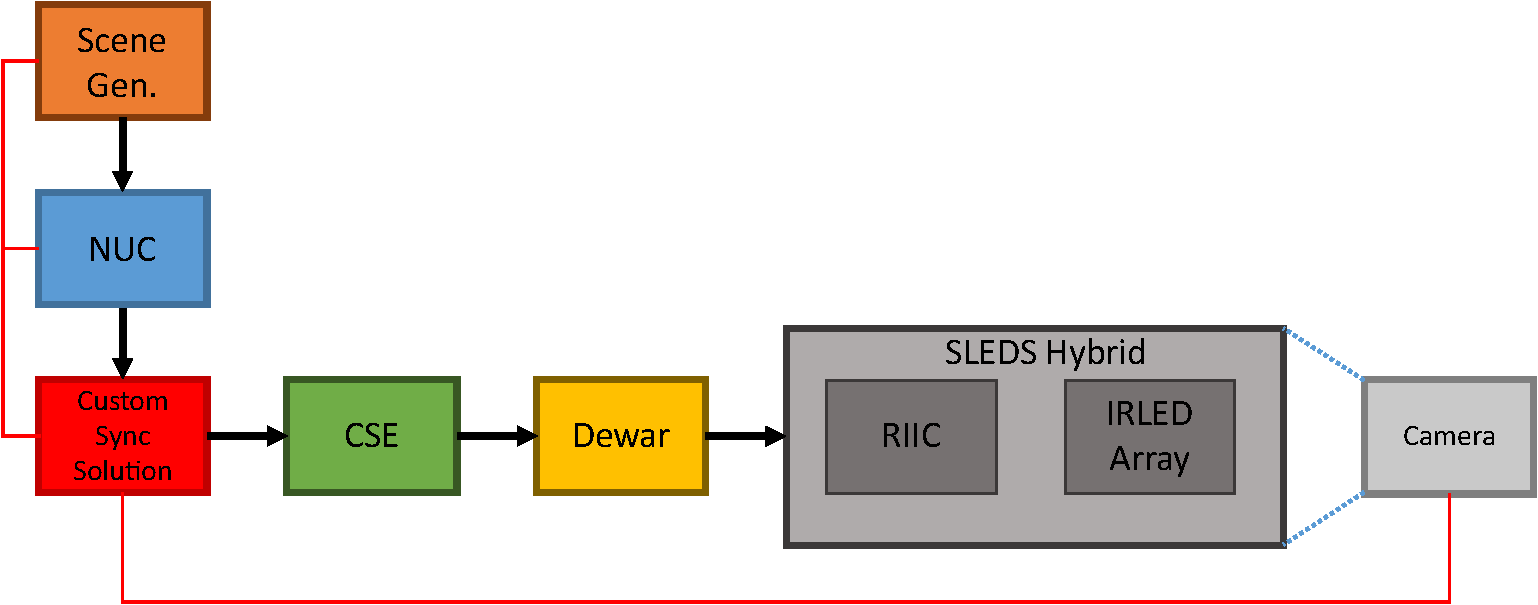
\includegraphics[width=1.0\textwidth]{fig/custom_sync.pdf}
        \caption{Custom Synchronization Solution}
        \label{fig:custom_sync}
    \end{figure}

    This can range from utilizing off the shelf components such as Nvidia Quadro Sync cards~\cite{NVIDIA2020_2} or developing additional hardware pipelines capable of buffering and delaying emission of frame data such as an intermediate buffer card. This presents a particular challenge because the user typically does not have direct control over frame buffers, frame emission, or the software drivers within a system when utilizing display protocol-based technology. Moreover, encoders and decoders expect the protocols to work in a defined way that modifications for enabling synchronization could run afoul of; thus, resulting in the need for non-standard encoder and decoder implementations.

    The PDP on the other hand, eases synchronization due to its nature of being packetized, which allows for controlled data to be sent when directed without the need for a custom synchronization solution. With a PDP based solution, a scene generator could simply synchronize to a camera (if necessary) and send frame data when required under its own direct control. Moreover, hardware links could be replaced in the future with faster technology without the need to design a new hardware specific solution for synchronization. The only requirement being that the protocol be utilized across the new link.

    Now that the background of display protocols has been discussed, Chapter~\ref{chap:pdp_protocol} shifts focus to a discussion of the design of the PDP itself followed by a protocol specification. Some of the more protocol specific details left out here, such as variable refresh rate (VRR), are discussed there to provide a comparison with PDP features.

    \chapter{Packetized Display Protocol}
        \label{chap:pdp_protocol}

%$FIXME: wrong now
This chapter discusses the underlying communication details of the packetized display protocol (PDP) architecture. First, it gives an overview of the protocol design methodology. Secondly, it provides comparison with conventional display technology. Thirdly, it discusses requirements for packet formatting. Fourthly, it discusses individual packet types. Fifthly, it delves into the overhead of utilizing PDP packets. Sixthly, it discusses multi-frame rate performance within the PDP through an example of a dual frame rate operation. The central purpose of this chapter is to provide the reader with an understanding of the reasoning behind design decisions as well as to provide a detailed specification of the protocol and its performance characteristics when utilized in different scenarios.

\section{Design Methodology}
    \label{sec:design_methodology}
    This section discusses the design methodology for the PDP Protocol which began with a number of critical design goals~\cite{LandwehrEtAl2019}. An attempt to address the goals is not presented directly here but discussed  elsewhere due to it being a complex topic with many interwoven aspects. The design goals are as follows:

    \begin{enumerate}
        \item {\em To design a scalable display system that is distributable and hardware agnostic.} The display protocols and interfaces utilized within projector systems have systematic issues with remaining up to date with current technology in that old standards (such as DVI) continue to be utilized due to the inability for custom synchronization solutions to work with newer hardware as well as due to the costs and time associated with implementing newer solutions utilizing newer standards. This will be touched upon throughout this chapter and discussed more extensively in Chapter~\ref{chap:machine_model}.
        \item {\em To provide a protocol that is relatively simple to implement without unnecessary complexity to ease the encoding and decoding process.} A low overhead and fast decode process is crucial to ensuring latency is sub-frame\footnote{This refers to latency of that below the time it would take to buffer an entire frame. Which is a common synchronization method utilized in projector systems.} across an end-to-end system. Additionally, simplifying these processes also eases potential hardware implementation mistakes as well as inefficiencies that could lead to reduced performance. This will be touched upon in Chapters~ \ref{sec:packet_format},~\ref{sec:packet_types}, and~\ref{sec:pdp_stream_decoding}.
        \item {\em To provide dynamic intra-frame variable refresh rate (VRR) in order to enable better bandwidth utilization.} In particular, to allow for regions of a display to be intelligently updated at different rates when driven by a scene generator. This will be discussed upon in Chapters~\ref{sec:multi_framerate_performance} and \ref{sec:compositing}.
        \item {\em To provide a path to utilize conventional display protocol streams such as HDMI as a backwards compatible transport layer for PDP without introducing overhead.} This is to allow for interoperability where necessary when utilizing conventional display sources, and to ease migration to a PDP based system. This will be touched upon in Chapter~\ref{sec:pdp_stream_decoding}, and discussed more extensively in Chapter~\ref{chap:implementation}.
    \end{enumerate}

    For methodology, each goal was considered when making decisions about what should and should not be part of the PDP, and where the boundaries of the protocol should lie. This included such decisions as how to incorporate hardware specific features, the best method to support VRR without constraining the methods by which users can implement support for it within scene generators\footnote{VRR implemented within HDMI and DisplayPort is driver controlled and thus the user has no ability to control it.}, and how to ease implementation in current and future hardware. Hardware specific optimizations can be important for performance reasons even in hardware agnostic protocols. Therefore, it is paramount to make hardware agnostic protocols general enough to support various configurations. For example, tuning within TCP~\cite{WeigleFeng2002} is a well-known important consideration in the field of networks for maximizing throughput due to differing hardware and network topologies. In PDP, one example of a hardware specific feature that needs consideration is the support for different array write processes\footnote{See Chapter~\ref{chap:array_write_process} for the interleaved array write process of the NSLEDS and HDILED arrays.} because efficient ordering of data is important for low latency operation and minimizing hardware complexity.

\section{Comparison}

    To better understand how to design PDP, the constraints of conventional display protocols were investigated to discern which features within these protocols conflict with the design goals of PDP. In addition, it was necessary to investigate whether these could provide a path forward in the design and development of PDP. Many versions of these protocols (DVI~\cite{DDWG1999}, HDMI~\cite{HDMIForum2018}, DisplayPort~\cite{VESA2016}, etc.) provide similar feature-sets to end-users with the major focus being on increasing refresh rates and resolutions with each new specification. However, as discussed in Chapter~\ref{sec:conventional_display_protocols}, their basis is rooted in classical analog video specifications that utilize scan lines~\cite{Neal1998}. This means that signal timing utilizes vertical and horizontal blanking periods that consist of a front-porches, sync pulses, and back-porches; in addition to, the active video data to be displayed.

    For early analog display devices, these signals enabled operators to manually adjust horizontal and vertical hold times relative to the sync pulses to correct for the imprecise timing of early display hardware; but provide little benefit on modern hardware other than as an embedded method to support sending frames at a static interval, and to enable tearless buffer swapping in either double buffering~\cite{FriedbergEtAl1990} or triple buffering schemes~\cite{3dfx1997} utilized within GPUs\footnote{This is performed by swapping buffers during the vertical sync (vsync) interval of a frame~\cite{3dfx1999,3dfx1999_2}. See Chapter~\ref{chap:display_protocols} for details about vsync intervals.}.

    In digital display technology, embedded blanking periods represent an anachronism that impedes the goal of maximizing bandwidth utilization when driving a display by requiring the transmission of unnecessary data over digital protocols. For example, a commonly utilized 1920 by 1080 pixel mode operating at \mbox{60 Hz}~\cite{MythTV2015} on a modern display has a 16 percent blanking period overhead due to the specification of vertical and horizontal sync periods. Other examples can be seen in Table~\ref{tbl:modeline_overhead}. Of note, modes with {\it 512 by 512} and {\it 512 by 256} visible pixels are non-standard and were tested on existing hardware to minimize the overhead of blanking. Additionally, these have been utilized within NSLEDS and TCSA during actual array operation. What one sees is that as modelines shrink and data rates decrease, the percentage of blanking relative to displayed pixels significantly increases. This is due to the inability for common implementations of video decoders to operate correctly when blanking is minimized. An additional issue is that when non-standard visible resolutions are utilized many decoders do not operate at all.

    \begin{table}
        \centering
        \large
        \begin{tcolorbox}[tabularx={Y|Y|Y|Y|Y},title=\textbf{Modeline Overhead},boxrule=0.5pt]
        \textbf{\normalsize Resolution} & \textbf{\normalsize Refresh Rate (Hz)} & \textbf{\normalsize Visible Pixels} & \textbf{\normalsize Total Pixels} & \textbf{\normalsize Overhead} \\ \hline
            \textbf{\normalsize 1920x1080} & \textbf{\normalsize 60}   & {\normalsize 2073600} & {\normalsize 2475000} & {\normalsize 16.2\%} \\ \hline
            \textbf{\normalsize 1600x1200} & \textbf{\normalsize 60}   & {\normalsize 1920000} & {\normalsize 2700000} & {\normalsize 28.9\%} \\ \hline
            \textbf{\normalsize 1280x1024} & \textbf{\normalsize 60}   & {\normalsize 1310720} & {\normalsize 1799408} & {\normalsize 27.2\%} \\ \hline
            \textbf{\normalsize 1280x960}  & \textbf{\normalsize 60}   & {\normalsize 1228800} & {\normalsize 1800000} & {\normalsize 31.7\%} \\ \hline
            \textbf{\normalsize 1280x800}  & \textbf{\normalsize 60}   & {\normalsize 1024000} & {\normalsize 1391040} & {\normalsize 26.4\%} \\ \hline
            \textbf{\normalsize 1024x768}  & \textbf{\normalsize 60}   & {\normalsize 786432 } & {\normalsize 1083264} & {\normalsize 27.4\%} \\ \hline
            \textbf{\normalsize 512x512}   & \textbf{\normalsize 500}  & {\normalsize 262144 } & {\normalsize 296100 } & {\normalsize 11.5\%} \\ \hline
            \textbf{\normalsize 512x512}   & \textbf{\normalsize 400}  & {\normalsize 262144 } & {\normalsize 296100 } & {\normalsize 11.5\%} \\ \hline
            \textbf{\normalsize 512x512}   & \textbf{\normalsize 300}  & {\normalsize 262144 } & {\normalsize 357500 } & {\normalsize 26.7\%} \\ \hline
            \textbf{\normalsize 512x512}   & \textbf{\normalsize 100}  & {\normalsize 262144 } & {\normalsize 357500 } & {\normalsize 26.7\%} \\ \hline
            \textbf{\normalsize 512x512}   & \textbf{\normalsize 60}   & {\normalsize 262144 } & {\normalsize 357500 } & {\normalsize 26.7\%} \\ \hline
            \textbf{\normalsize 512x512}   & \textbf{\normalsize 50}   & {\normalsize 262144 } & {\normalsize 364000 } & {\normalsize 28.0\%} \\ \hline
            \textbf{\normalsize 512x512}   & \textbf{\normalsize 30}   & {\normalsize 262144 } & {\normalsize 520000 } & {\normalsize 50.0\%} \\ \hline
            \textbf{\normalsize 512x512}   & \textbf{\normalsize 30}   & {\normalsize 262144 } & {\normalsize 520000 } & {\normalsize 50.0\%} \\ \hline
            \textbf{\normalsize 512x256}   & \textbf{\normalsize 1000} & {\normalsize 131072 } & {\normalsize 149460 } & {\normalsize 12.3\%} \\ \hline
            \textbf{\normalsize 512x256}   & \textbf{\normalsize 500}  & {\normalsize 131072 } & {\normalsize 256000 } & {\normalsize 48.8\%} \\ \hline
            \textbf{\normalsize 512x256}   & \textbf{\normalsize 200}  & {\normalsize 131072 } & {\normalsize 320000 } & {\normalsize 59.0\%} \\ \hline
            \textbf{\normalsize 512x256}   & \textbf{\normalsize 100}  & {\normalsize 131072 } & {\normalsize 320000 } & {\normalsize 59.0\%} \\ \hline
            \textbf{\normalsize 512x256}   & \textbf{\normalsize 60}   & {\normalsize 131072 } & {\normalsize 320000 } & {\normalsize 59.0\%} \\ \hline
        \end{tcolorbox}
        \caption[Modeline Overhead]{Modeline overhead for various resolutions and refresh rates~\cite{MythTV2015}. Computed using active pixel area over total pixel area. 512x512 and 512x256 are typical modeline resolutions used on IRLED arrays.}
        \label{tbl:modeline_overhead}
    \end{table}

    These protocols also internally utilize a mode based display of data that requires the specification of the absolute width and height of display as well as a pixel clock which when used in conjunction with the vertical blanking information provides a total refresh rate as described in Chapter~\ref{sec:conventional_display_protocols}. This means that the bandwidth requirements for a given mode are inherently static across all frames. In addition, this constrains the refresh rate for a display to be static in terms of both the intra-frame regions of the display and between frames. Effectively increasing the burden of synchronization and impeding the introduction of dynamism into the display process.

    In recent years, work has been done to implement a limited form of variable refresh rate (VRR) display between frames for use with newer protocols~\cite{AMD2019,NVIDIA2020_1}. In essence, it allows for entire frames to be sent for display immediately once the rendering process has completed. A downside is that historically this has generally required specialized hardware support out of the scope of protocol specifications. A recent update of the HDMI 2.1 specification~\cite{HDMIForum2018} has integrated a speed-limited form of VRR directly into the specification that requires full frames of data to be transmitted at a statically specified resolution and target frame rate. DisplayPort provides a similar form of VRR~\cite{VESA2014} with a similar set of limitations which also require full frames of data to be transmitted at a specified resolution and target frame rate.

    DisplayPort differs from older display standards in that data streams themselves are framed~\cite{VESA2011,Wiley2011}, though the standard itself refers to this framing as packetization it differs from the normal sense of packets in that arbitrary packets of data with dynamic meanings and decoding cannot be sent. An example of the framing is shown in Figure~\ref{fig:display_port_framing}. Once per frame in between pixel data, a {\it blanking start} symbol is inserted into the data stream to indicate the start of vertical blanking. Then, a {\it Main Stream Attribute (MSA)} packet is sent that contains the total number of horizontal pixels per line, the total number lines, the start of active video pixels relative to hsync, the start of active lines relative to vsync, and the pixel formatting. After which, a {\it blanking end} symbol is inserted to indicate the end of vertical blanking. Following this, pixel data conforming to the video specification within the MSA packet is sent along with {\it stuffing} symbols that are framed with {\it fill start} and {\it end} symbols. These can be of different lengths and are used to represent space between actual data. After all the data for a frame is sent, {\it blanking} symbols for the next frame occur, and the process repeats. In essence, what DisplayPort provides is a framed method of sending video formatting information per frame instead of embedding these signals in a separate synchronized stream. Display port also provides a secondary stream to send audio or other information (not shown) during the blanking interval similar to how blanking intervals are sometimes used as a side channel for extra data in earlier protocols.

    \begin{figure}
        \centering
        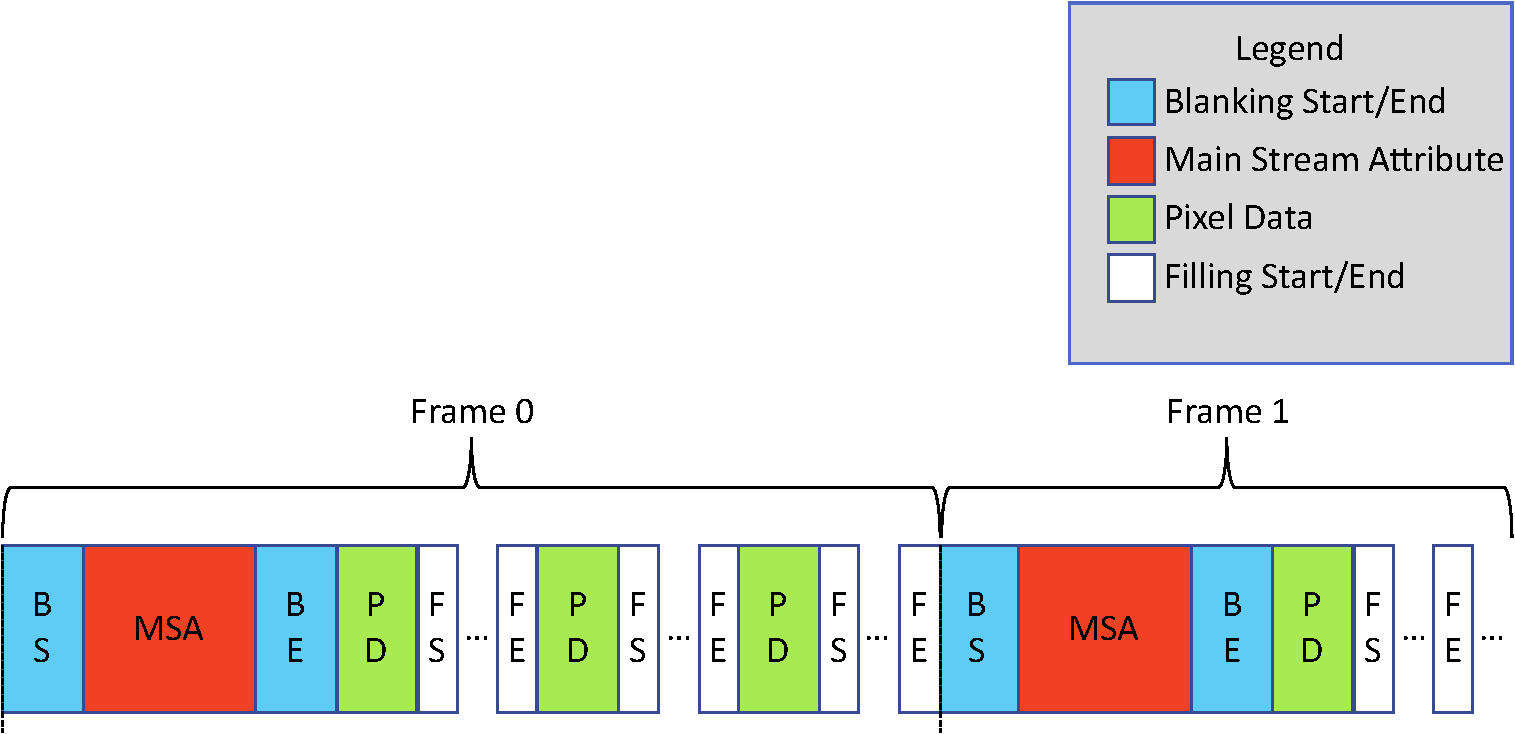
\includegraphics[width=1.0\textwidth]{fig/display_port_framing.pdf}
        \caption{Display Port Framing}
        \label{fig:display_port_framing}
    \end{figure}

    This differs from PDP in that PDP allows for completely arbitrary packets to be sent and decoded with differing packet sizes which gives PDP the ability to support dynamic sub-frame frame rates, and to be extendable to future packet types. Additionally, PDP carries no internal notion of horizontal or vertical blanking intervals which allows PDP to operate as fast as possible and give scene generators direct control over frame rates at the user level. For example, the transport upon which PDP is implemented can operate at the maximum possible data rate allowable in hardware; then, the user in turn can simply send packets over the data link at the desired rate while inserting empty space where necessary. In the backend, a PDP decoder would decode the data as quickly as possible and display it. From a higher level, this could be viewed as the user simply issuing commands to send data packets similar to that of how TCP based programs send data over a link with a remote environment executing the actual commands. It is up to the user where and when they want data displayed which enables PDP to fit a larger set of use cases, and to be simpler to integrate within projector systems.

\section{Packet Format}
    \label{sec:packet_format}
    Given the goals discussed in Chapter~\ref{sec:design_methodology}, it is important to discuss different considerations for packet formatting within the PDP. At a minimum PDP needs a method to be able to write to different regions of a display in insolation from other regions. For that minimal set of data that needs to be encoded is an x start address, y start address, x end address, y end address, and the pixels data. Additionally, these fields need to be able to be efficiently encodable and decodable as well as minimize the necessary intermediate operations required for manipulating the data in both backend architectures (close to an array), and front-end architectures (close to scene generator). Moreover, the bit-width is important both in terms of encoding/decoding efficiency and rollover. The latter, due to the maximum sizes and arrays could reach in terms of resolution.

    Given that majority of off the shelf computer hardware architectures are at least byte aligned or 8-bit aligned in terms of instruction set architecture (ISA) and bus widths, it is prudent to consider data alignment. This is primarily due to unaligned data requiring additional operations such as bit shifting and masking in order to manipulate it within the majority of modern architectures. For example, a multiplication of a 6-bit width data may require storing the result in an 8-bit word and masking the two upper bits to zero before the multiplication operation is performed.

    The coordinate system being utilized within the PDP is another important consideration because sub-optimal choices could lead to unnecessary translations which increase operation costs and computational complexity for manipulating data. For example, if one were to store the beginning X coordinate within a packet with a coordinate offset for the range instead of the end coordinate itself, then computing the ending coordinate for the range would require an addition on the backend. And potentially, $2N^2$ additional mathematical operations to allow comparing region boundaries if PDP were being composited where N is the number of independent regions to draw.

\section{Packet Types}
    \label{sec:packet_types}
    Table~\ref{tbl:packets} shows the basic packets used for communication within the PDP. These are strictly for data transfer and synchronization of system operations, and do not include other aspects such as system setup or enumeration\footnote{System setup and enumeration are typically system specific operations and outside of the current PDP Design but may be incorporated in the future.}. These packets are organized into type specific fields of some set word-size. The exact size of word fields is left abstracted to allow for an optimal implementation to be used in practice. For example, a system may utilize 24-bit word size if an array has a native 24-bit pixel size, or 32-bit word size if the hardware transport layer has a specific optimal word size. Typically, a multiple of 8-bit word size would be utilized in practice, as most hardware architectures (such as x86) utilize some multiple of this size\cite{HennessyEtAl2012}. In any given implementation, the word size of all fields must match, in order to simplify decoding operations. This allows for fixed-size decoding of incoming data, which simplifies processing and firmware implementation as well as can ease timing constraints and enforce non-variability in the decoding time of incoming packets of data. In general, PDP packets are designed to send a minimal amount of header data to lower overhead and are ordered in a way to minimize buffering requirements in order to enable real-time processing.

    \begin{table}
        \centering
        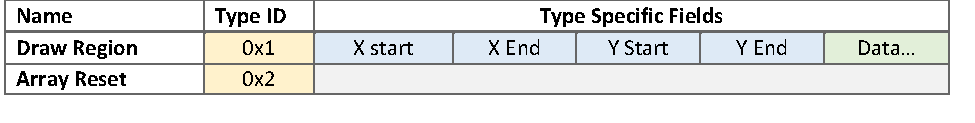
\includegraphics[width=1.0\textwidth]{fig/packet_chart.pdf}
        \caption{List of PDP Packets}
        \label{tbl:packets}
    \end{table}

    In terms of the protocol itself, PDP uses a single global coordinate system to refer to pixel locations on a display array. For example, a 512 by 512 pixel array would have coordinates from 0 to 511 in both the horizontal and vertical directions. All packets referencing sub-regions of this display would utilize coordinates that map to some rectangular sub-region of the display. Any overlapping regions of data would be composited during system operation with the compositor giving priority to data segments that need to be displayed at higher frame rates.

    PDP Packets are divided into four types, a no operation packet, a draw region packet, array reset packet, and trigger packet. All packets consist of a Type ID field of word-size. The type ID is used by the decoder to determine the packet type.

    The first packet type, {\it No Operation}, is simply indicating that command IDs of 0x0 will be ignored.

    The second packet type, {\it Draw Region}, is used to send a rectangular sub-region of pixel data in global array coordinates to minimize computations and translations. It has fields for the start and stop horizontal and vertical coordinates (defined inclusively) followed by individual pixel data. For example, suppose a scene generator were to send a packet of data from array region 10 to 19 along the X axis and 20 to 29 along the Y axis, a total of 100 pixels of data would follow the packet coordinates given that the packet specifies a 100 pixel sized region.

    The third packet type, {\it Array Reset}, is utilized to indicate that quadrants on a given array should be cleared. The causes a quadrant to stop displaying its current contents. It consists of an array specific quadrant bitmask used to indicate which quadrant to reset. Any unused bits are reserved. This type of packet would be utilized exclusively to control clearing of quadrants which may be necessary on certain types of array architectures.

    The fourth packet type, {\it Trigger}, could be used to implement a trigger-based synchronization within the PDP. It consists of a system specific action bitmask used to indicate the type of operation to trigger. In IRLED array systems, the coordinator of synchronization is dependent on the array itself and the different components within the system. In some systems, a sensor may be used as the source of synchronization, in other systems, another component may be utilized. Other aspects of system operation may even be triggered outside of the system synchronization interval based off other events. For this reason, PDP has opted for a trigger-based approach to synchronization. This approach allows for synchronization, data transfer, and computation to be custom tailored for specific use cases. For example, the action mask could be used to trigger the generation of the next frame to be displayed when needed, the source of which is defined by the system itself. Another example would be to utilize the action mask to indicate that further computations (such as scene generation) stall until otherwise indicated.

\section{PDP Stream Decoding}
    \label{sec:pdp_stream_decoding}
    In this section, a discussion of how PDP might operate with actual data is provided to aid the reader with understanding of how packets are envisioned to be decoded and how a generalized write process to an array may occur. An actual implementation of PDP on a real system is discussed in Chapter~\ref{chap:implementation} with experimental results discussed in Chapter~\ref{chap:experimental_results}.

    Figure~\ref{fig:pdp_stream} demonstrates a PDP stream for an architecture with a minimum write size of four pixels and a column-first write order. Represented is the streaming of each word within a PDP packet. Time is represented moving downwards with the internal PDP state and buffer data changing as each word is streamed in.

    \begin{figure}
        \centering
        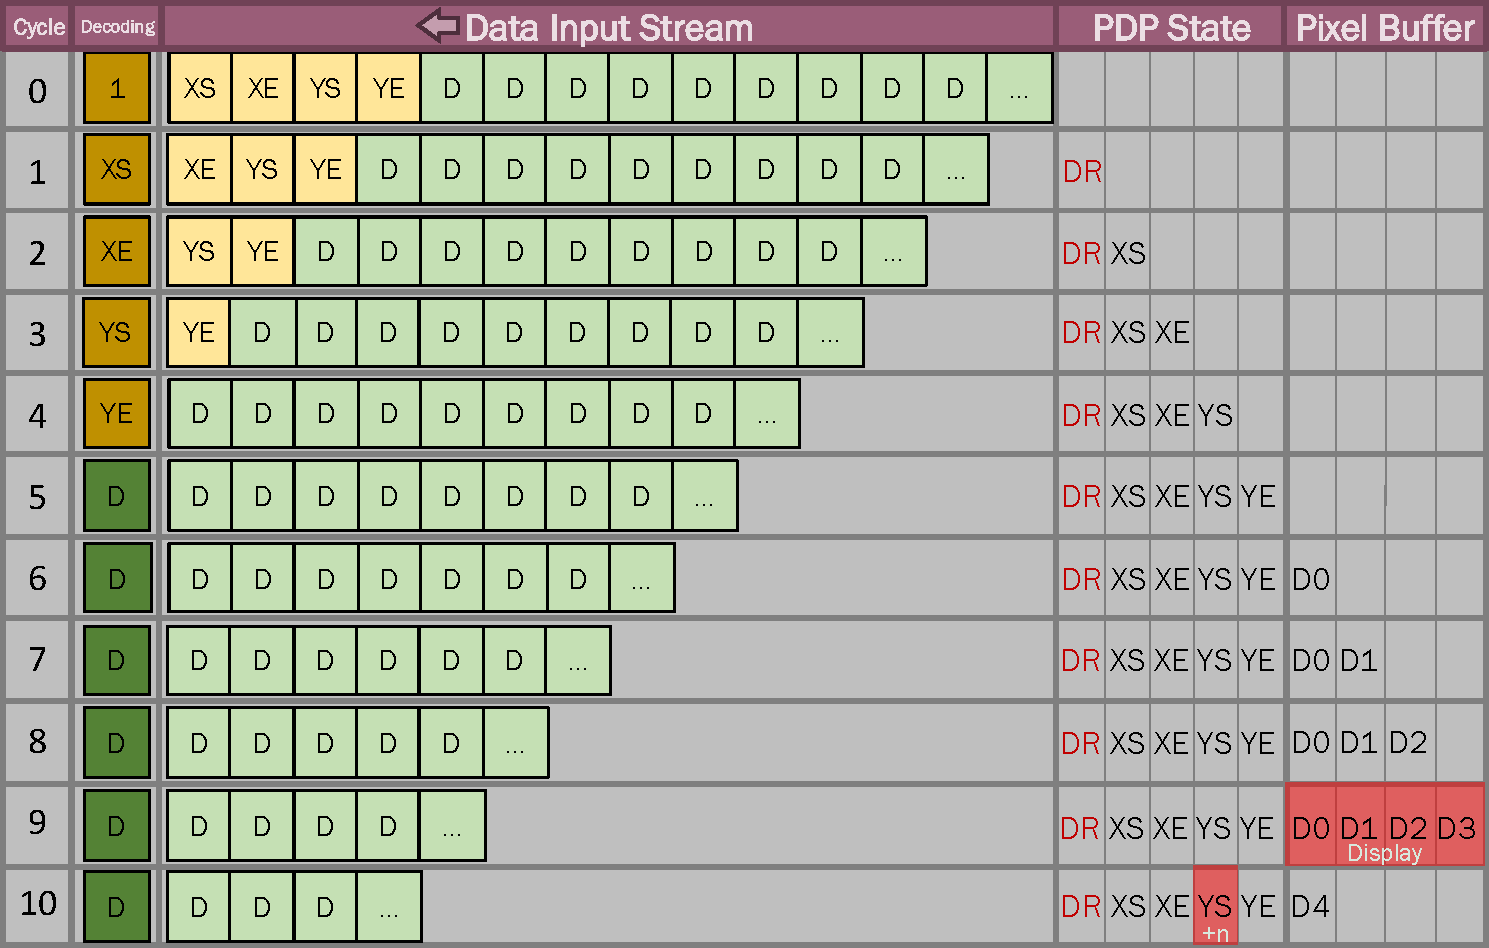
\includegraphics[width=1.0\textwidth]{fig/pdp_stream.pdf}
        \caption{Example PDP Stream}
        \label{fig:pdp_stream}
    \end{figure}

    {\it One} is the opcode for a draw region packet which is denoted as {\it DR} in the diagram. {\it XS} stands for x start. {\it XE} stands for x end. {\it YS} stands for y start. {\it YE} stands for y end. These are the header words for a PDP draw region packet. {\it D} stands for data which represents each pixel word to draw to an array. At the beginning of time, PDP state is empty. Once the opcode is read in, PDP would enter the draw region state. Then each word for the region boundaries would be read in one by one until entire header has been parsed. Next, pixel data is streamed in starting with {\it D0}. Once all the words necessary for a single array draw are buffered in, which in the case of the example architecture, is four pixels, the buffered data is then written to the array as indicated. Following this, {\it YS} is incremented to move to the next address on the array\footnote{Array write processes can differ as indicated in Chapter~\ref{sec:array_Interleaved_write_process}, due to this the index {\it n} in Figure~\ref{fig:pdp_stream} is an array specific value that indicates the amount by which to increment {\it YS}. In architectures with a row-first write order, {\it XS} may be incremented instead.}, and {\it D4} is buffered in. The buffering and writing process is continued until the end of the column when {\it YS} equals {\it YE}. Then {\it XS} would be incremented and {\it YS} reset to the start of the region. Then each column would be buffered and written in the same manner as the first until {\it YS} equals {\it YE} and {\it XS} equals {\it XE}, which indicates the end of the frame. After this, a new packet would be streamed in and decoded in the same manner.

    One important note about the decoding process discussed here is that it would be relatively simple to implement by utilizing a state machine within hardware that encapsulates the different PDP state variables. A major factor in this is the fixed width word size utilized within the PDP. Fixed width decoding means that partial words do not need to be buffered, and dynamic buffers and routing need not be utilized within a decoder. As discussed in Chapter~\ref{sec:design_methodology}, one of the design goals of PDP is to provide a means to ease implementation complexity. This simplification of hardware implementation allows for resources to be focused on optimally routing data in and out of the an FPGA, ASIC, or other implementations while minimizing timing closure issues in an environment where a major challenge is the plethora of signals that need to be routed. For example, within NSLEDS and HDILED based systems, it is necessary to route 512 data lines due to the 32 16-bit DAC channels used. Future systems could double that number to 1024 by utilizing 64 16-bit DAC channels.

    As one of the goals of PDP is to provide backwards compatibility, an important consideration is how this decoding process might be implemented within a display protocol transport layer. Most of the details regarding this will be discussed in Chapter~\ref{sec:hdmi_transport_layer}, for now, it is worth noting that for an implementation that is backwards compatible with HDMI, draw packet headers could be transmitted by a secondary data channel leaving the main stream channel for pixel data. This would allow for pixels data to be transmitted exactly as normal while utilizing normal display protocol modelines, thus, allowing users to be able to utilize their array technology transparently as-is without any changes while utilizing an array that internally supports PDP via its close support electronics.

\section{Overhead}
    As mentioned previously, internally PDP has no notion of blanking periods or porches for providing synchronization, and therefore does not encapsulate the inefficiencies inherent in the aforementioned protocols. Instead synchronization and frame rates within the PDP are controlled by the source through timing when data is sent. This means that high overheads due to blanking can be mitigated. Table~\ref{tbl:pdp_efficiency} shows the maximum packet overhead due to packet encapsulation when PDP is utilized for the same resolutions and frequencies listed in Table~\ref{tbl:modeline_overhead}. These are computed using active pixel area over total pixel area. The right column shows the reduction in overhead vs normal modelines. {\it 512 by 512} and {\it 512 by 256} are typical modeline resolutions used on IRLED arrays. These numbers represent a worst-case scenario when PDP is implemented within a transport layer that does not require blanking intervals. In actual usage, larger packets consisting of more pixels would be utilized therefore, the overhead would be lower on average. However, even in worst-case scenarios PDP has a vast reduction on bandwidth requirements on average which means that faster refresh rates can be utilized in bandwidth limited situations. Additionally, higher interation times could be utilized within IR cameras and sensors due to less time being needed for writing the same visible data to an IR array. For example, with the 512 by 256 modeline operating at 200Hz, integrations times could be increased by up to 51.8 percent over a traditional modeline.

    \begin{table}
        \centering
        \large
        \begin{tcolorbox}[tabularx={Y|Y|Y|Y|Y|Y},title=\textbf{PDP Maximum Packet Overhead},boxrule=0.5pt]
        \textbf{\normalsize Slow Refresh Rate (Hz)} & \textbf{\normalsize Fast Refresh Rate (Hz)} & \textbf{\normalsize Visible Pixels} & \textbf{\normalsize Total Pixels} & \textbf{\normalsize Overhead} & \textbf{\normalsize Overhead Reduction} \\ \hline
            \textbf{\normalsize 1920x1080} & \textbf{\normalsize 60}   & {\normalsize 2073600} & {\normalsize 2235600} & {\normalsize 7.2\%} &\textbf{\normalsize 9.0 \%} \\ \hline
            \textbf{\normalsize 1600x1200} & \textbf{\normalsize 60}   & {\normalsize 1920000} & {\normalsize 2070000} & {\normalsize 7.2\%} &\textbf{\normalsize 21.7\%} \\ \hline
            \textbf{\normalsize 1280x1024} & \textbf{\normalsize 60}   & {\normalsize 1310720} & {\normalsize 1413120} & {\normalsize 7.2\%} &\textbf{\normalsize 20.0\%} \\ \hline
            \textbf{\normalsize 1280x960}  & \textbf{\normalsize 60}   & {\normalsize 1228800} & {\normalsize 1324800} & {\normalsize 7.2\%} &\textbf{\normalsize 24.5\%} \\ \hline
            \textbf{\normalsize 1280x800}  & \textbf{\normalsize 60}   & {\normalsize 1024000} & {\normalsize 1104000} & {\normalsize 7.2\%} &\textbf{\normalsize 19.2\%} \\ \hline
            \textbf{\normalsize 1024x768}  & \textbf{\normalsize 60}   & {\normalsize 786432 } & {\normalsize 847872 } & {\normalsize 7.2\%} &\textbf{\normalsize 20.2\%} \\ \hline
            \textbf{\normalsize 512x512}   & \textbf{\normalsize 500}  & {\normalsize 262144 } & {\normalsize 282624 } & {\normalsize 7.2\%} &\textbf{\normalsize 4.3\% } \\ \hline
            \textbf{\normalsize 512x512}   & \textbf{\normalsize 400}  & {\normalsize 262144 } & {\normalsize 282624 } & {\normalsize 7.2\%} &\textbf{\normalsize 4.3\% } \\ \hline
            \textbf{\normalsize 512x512}   & \textbf{\normalsize 300}  & {\normalsize 262144 } & {\normalsize 282624 } & {\normalsize 7.2\%} &\textbf{\normalsize 19.5\%} \\ \hline
            \textbf{\normalsize 512x512}   & \textbf{\normalsize 100}  & {\normalsize 262144 } & {\normalsize 282624 } & {\normalsize 7.2\%} &\textbf{\normalsize 19.5\%} \\ \hline
            \textbf{\normalsize 512x512}   & \textbf{\normalsize 60}   & {\normalsize 262144 } & {\normalsize 282624 } & {\normalsize 7.2\%} &\textbf{\normalsize 19.5\%} \\ \hline
            \textbf{\normalsize 512x512}   & \textbf{\normalsize 50}   & {\normalsize 262144 } & {\normalsize 282624 } & {\normalsize 7.2\%} &\textbf{\normalsize 20.8\%} \\ \hline
            \textbf{\normalsize 512x512}   & \textbf{\normalsize 30}   & {\normalsize 262144 } & {\normalsize 282624 } & {\normalsize 7.2\%} &\textbf{\normalsize 42.8\%} \\ \hline
            \textbf{\normalsize 512x512}   & \textbf{\normalsize 30}   & {\normalsize 262144 } & {\normalsize 282624 } & {\normalsize 7.2\%} &\textbf{\normalsize 42.8\%} \\ \hline
            \textbf{\normalsize 512x256}   & \textbf{\normalsize 1000} & {\normalsize 131072 } & {\normalsize 141312 } & {\normalsize 7.2\%} &\textbf{\normalsize 5.1\% } \\ \hline
            \textbf{\normalsize 512x256}   & \textbf{\normalsize 500}  & {\normalsize 131072 } & {\normalsize 141312 } & {\normalsize 7.2\%} &\textbf{\normalsize 41.6\%} \\ \hline
            \textbf{\normalsize 512x256}   & \textbf{\normalsize 200}  & {\normalsize 131072 } & {\normalsize 141312 } & {\normalsize 7.2\%} &\textbf{\normalsize 51.8\%} \\ \hline
            \textbf{\normalsize 512x256}   & \textbf{\normalsize 100}  & {\normalsize 131072 } & {\normalsize 141312 } & {\normalsize 7.2\%} &\textbf{\normalsize 51.8\%} \\ \hline
            \textbf{\normalsize 512x256}   & \textbf{\normalsize 60}   & {\normalsize 131072 } & {\normalsize 141312 } & {\normalsize 7.2\%} &\textbf{\normalsize 51.8\%} \\ \hline
        \end{tcolorbox}
        \caption{PDP Maximum Packet Overhead}
        \label{tbl:pdp_efficiency}
    \end{table}

    The numbers in Table~\ref{tbl:pdp_efficiency} are computed by taking the visible resolution and dividing it by the minimum pixel write size supported on an array. The minimum pixel write size is also synonymous with minimum possible PDP packet payload size excluding headers, and thus, is denoted as $S_{pkt}$. This yields the maximum possible packet count, $C_{pkt}$, for a given resolution as shown in Equation~\eqref{eq:packet_max}. The visible resolution parameters are denoted as horizontal active, $h_a$, and vertical active, $v_a$, respectively to keep consistent with the naming conventions used in Chapter~\ref{chap:display_protocols}. Within the NSLEDS and HDILED arrays, the minimal packet size, $S_{pkt}$, is 2 by 32 due to the interleaved array write process discussed in Chapter~\ref{chap:array_write_process}.

    \begin{equation}
        \begin{array}{ l }
            \displaystyle C_{pkt}=\frac{h_a \cdot v_a}{S_{pkt}} \\[13pt]
            \displaystyle C_{pkt}=\frac{h_a \cdot v_a}{2 \cdot 32}\\[13pt]
        \end{array}
        \label{eq:packet_max}
    \end{equation}

    The total pixel overhead, $O_{px}$, is computed by multiplying the total packet count, $C_{pkt}$, by the packet overhead, $O_{pkt}$, as shown in Equation~\eqref{eq:overhead_pixel}. The overhead is determined by looking at the total number of additional words added for PDP header data. Header details are discussed in Chapter~\ref{sec:packet_format}.

    \begin{equation}
        \begin{array}{ l }
            \displaystyle O_{px}=O_{pkt} \cdot C_{pkt} \\
            \displaystyle O_{px}=5\cdot C_{pkt} \\[13pt]
        \end{array}
        \label{eq:overhead_pixel}
    \end{equation}

    The total pixel count, $T_{px}$, is determined by adding the total pixel overhead, $O_{px}$, (or the result of Equation~\eqref{eq:overhead_pixel}) to the visible pixel size as shown in Equation~\eqref{eq:total_pixel}.

    \begin{equation}
        \begin{array}{ l }
            \displaystyle T_{px}=O_{pkt} \cdot C_{pkt} + h_a \cdot v_a \\
            \displaystyle T_{px}=O_{px} + h_a \cdot v_a \\
            \displaystyle T_{px}=5\cdot C_{pkt} + h_a \cdot v_a \\[13pt]
        \end{array}
        \label{eq:total_pixel}
    \end{equation}

    Putting the input variables together and simplifying yields Equation~\eqref{eq:total_pixel2} where $T_{px}$ is the total pixel count.

    \begin{equation}
        \begin{array}{ l }
            \displaystyle T_{px}=O_{pkt} \cdot \frac{h_a \cdot v_a}{S_{pkt}} + h_a \cdot v_a \\[13pt]
            \displaystyle T_{px}=h_a \cdot v_a \cdot (\frac{O_{pkt}}{S_{pkt}} + 1) \\[13pt]
            \displaystyle T_{px}=h_a \cdot v_a \cdot (\frac{5}{2 \cdot 32} + 1) \\[13pt]
        \end{array}
        \label{eq:total_pixel2}
    \end{equation}

    Computing the overhead percentage, $O_{pdp}$, is simply a matter of dividing the total pixel overhead, $O_{px}$, by the total pixels, $T_{px}$.

    \begin{equation}
        \begin{array}{ l }
            \displaystyle O_{pdp}=\frac{O_{pkt}\cdot C_{pkt}}{T_{px}} \cdot 100 \\[13pt]
            \displaystyle O_{pdp}=\frac{O_{px}}{T_{px}} \cdot 100 \\[13pt]
        \end{array}
        \label{eq:overhead}
    \end{equation}

    Due to the nature of the total pixel overhead being proportional to the visible pixel size for each resolution, the overhead percentage under worst-case conditions cancels out to a constant consisting of only a relationship between the minimum packet size and packet overhead.

    %FIXME: Add 3d graphic from wolfram alpha

    \begin{equation}
        \begin{array}{ l }
            \displaystyle O_{pdp}=\frac{O_{pkt}\cdot \frac{h_a \cdot v_a}{S_{pkt}}}{O_{pkt} \cdot \frac{h_a \cdot v_a}{S_{pkt}} + h_a \cdot v_a} \cdot 100 \\[16pt]
            \displaystyle O_{pdp}=\frac{O_{pkt}\cdot \frac{\cancelto{1}{h_a \cdot v_a}}{S_{pkt}}}{O_{pkt} \cdot \frac{\cancelto{1}{h_a \cdot v_a}}{S_{pkt}} + \cancelto{1}{h_a \cdot v_a}} \cdot 100 \\[25pt]
            \displaystyle O_{pdp}=\frac{O_{pkt}\cdot \frac{1}{S_{pkt}}}{O_{pkt} \cdot \frac{1}{S_{pkt}} + 1} \cdot 100 \\[16pt]
            \displaystyle O_{pdp}=\frac{\frac{O_{pkt}}{S_{pkt}}}{\frac{O_{pkt}}{S_{pkt}} + 1} \cdot 100 \\[19pt]
            \displaystyle O_{pdp}=\frac{O_{pkt}}{O_{pkt}+S_{pkt}} \cdot 100 \\[19pt]
            \displaystyle O_{pdp}=\frac{5}{5 + 2 \cdot 32} \cdot 100 \\[19pt]
            \displaystyle O_{pdp}=7.2 \\[13pt]
        \end{array}
        \label{eq:cancel}
    \end{equation}

    The overhead reduction in Table~\ref{tbl:pdp_efficiency} is computed by subtracting the PDP overhead from the overheads listed in Table~\ref{tbl:modeline_overhead}. It is worth restating for posterity that these numbers represent worst-case scenarios for PDP when implemented on top of a transport layer that does not require blanking intervals. If the underlying transport layer upon which PDP is implemented cannot function without additional overhead, then the performance would be worse in practice as is the case if PDP is utilized with a display protocol-based transport layer. However, in the case of display protocols, overhead can be minimized relative to normal non-PDP operation by utilizing the fastest frequency the hardware allows and minimizing modeline porches. This would enable PDP to use much smaller porches than normal modelines. Additionally, horizontal porch overhead can be mitigated by timing an array's inherit analog settling delays to occur during the porches. This can be done by ensuring that there is enough data for a write prior to a horizontal blanking period.

\section{Multi-framerate Performance}
    \label{sec:multi_framerate_performance}

    This section discusses the benefits of utilizing a PDP based approach for reaching high frame rates. In high performance systems, data movement~\cite{LeeEtAl1984}, bandwidth~\cite{LaiBaker1999}, and latency~\cite{ZhengEtAl2014} are of primary concern due to the nature of these typically impeding performance requirements. In many cases, minimizing data movement can vastly improve the performance of systems~\cite{BandyopadhyayCoyle2004,LiEtAl2009,Hall2020}. In real time systems~\cite{Kopetz2011}, such as IR projector systems, where end-to-end latency is important for driving arrays, and the observation of real-time IR behavior is important for characterizing temperature changes~\cite{ZhouEtAl2000} minimizing data movement, and choosing appropriate hardware with high bandwidth as well as low latency is extremely important.

    As detailed throughout this thesis, PDP allows for control over which individual segments of an array can be written to. This means that large amounts of bandwidth can be saved by updating parts of a frame at slower frame rates than other sections of a frame. In simplified dual frame rate setup, Equation~\eqref{eq:bandwidth_saved} and the subsequent simplification show how to compute the percentage of saved bandwidth, $b_s$, when operating some proportion of pixels at a slower rate than a given faster rate. The proportion of pixels operating at a slow frame rate is $p$, the fast frame rate is $r_f$, and the slow frame rate is $r_s$. The final simplified form is simply the percentage of pixels operating at a slow rate multiplied by the difference between the rates over the fast rate.

    \begin{equation}
        \begin{array}{ l }
            \displaystyle b_s=\left(1-\frac{(1-p)\cdot r_f + p\cdot r_s}{r_f}\right)\cdot 100 \\[16pt]
            \displaystyle b_s \cdot r_f=\left(r_f-r_f \cdot \frac{(1-p)\cdot r_f + p\cdot r_s}{r_f}\right)\cdot 100 \\[13pt]
            \displaystyle b_s \cdot r_f= (r_f - (1-p)\cdot r_f - p\cdot r_s)\cdot 100 \\[13pt]
            \displaystyle b_s \cdot r_f= (r_f - r_f + p \cdot r_f - p\cdot r_s)\cdot 100 \\[13pt]
            \displaystyle b_s \cdot r_f= (p \cdot r_f - p\cdot r_s)\cdot 100 \\[13pt]
            \displaystyle b_s \cdot r_f= (p \cdot (r_f - r_s))\cdot 100 \\[13pt]
            \displaystyle b_s=\left(\frac{p \cdot (r_f-r_s)}{r_f}\right)\cdot 100
        \end{array}
        \label{eq:bandwidth_saved}
    \end{equation}

    Table~\ref{tbl:multi_framerate_bandwidth_savings} shows various examples of the bandwidth saved relative to operating all pixels at a given fast frame rate for PDP operation when two frame rates are utilized. The results are computed using Equation~\eqref{eq:bandwidth_saved} to give the reader an understanding of the kinds of savings that are possible by utilizing this method of operation. Of note, driving just half of the pixels at a slow rate can save near 50 percent of the bandwidth in these scenarios. This is of particular importance because many types of IR test scenarios utilized in practice contain sparse objects with low intensity backgrounds. In these types of scenarios, the bandwidth reduction would translate into the ability to display fast imagery at much higher rates than possible with conventual display technology. Indeed, display of small objects could have bandwidth reductions of over 95 percent. While these equations demonstrate a simplified use case for PDP, they provide a powerful argument for why the intra-frame variable refresh rate technology within the PDP has the potential to provide orders of magnitude better performance in bandwidth starved environments. In practice, many current projector systems struggle to achieve frame Rates above 200Hz due to the inability to deliver data at higher rates when utilizing conventional display technology.

    \begin{table}
        \centering
        \large
        \begin{tcolorbox}[tabularx={Y|Y|Y|Y},title=\textbf{Multi-frame Rate Bandwidth Savings},boxrule=0.5pt]
        \textbf{\normalsize Slow Frame Rate (Hz)} & \textbf{\normalsize Fast Frame Rate (Hz)} & \textbf{\normalsize Proportion of Slow Pixels (p)} & \textbf{\normalsize Bandwidth Saved (\%)} \\ \hline
            \textbf{\normalsize 10} & \textbf{\normalsize 100} & {\normalsize 0.1} & {\normalsize 9.0} \\ \hline
            \textbf{\normalsize 10} & \textbf{\normalsize 100} & {\normalsize 0.2} & {\normalsize 18.0} \\ \hline
            \textbf{\normalsize 10} & \textbf{\normalsize 100} & {\normalsize 0.3} & {\normalsize 27.0} \\ \hline
            \textbf{\normalsize 10} & \textbf{\normalsize 100} & {\normalsize 0.4} & {\normalsize 36.0} \\ \hline
            \textbf{\normalsize 10} & \textbf{\normalsize 100} & {\normalsize 0.5} & {\normalsize 45.0} \\ \hline
            \textbf{\normalsize 10} & \textbf{\normalsize 100} & {\normalsize 0.6} & {\normalsize 54.0} \\ \hline
            \textbf{\normalsize 10} & \textbf{\normalsize 100} & {\normalsize 0.7} & {\normalsize 63.0} \\ \hline
            \textbf{\normalsize 10} & \textbf{\normalsize 100} & {\normalsize 0.8} & {\normalsize 72.0} \\ \hline
            \textbf{\normalsize 10} & \textbf{\normalsize 100} & {\normalsize 0.9} & {\normalsize 81.0} \\ \hline
            \textbf{\normalsize 10} & \textbf{\normalsize 100} & {\normalsize 1.0} & {\normalsize 90.0} \\ \hline
            \textbf{\normalsize 10} & \textbf{\normalsize 1000} & {\normalsize 0.1} & {\normalsize 9.9} \\ \hline
            \textbf{\normalsize 10} & \textbf{\normalsize 1000} & {\normalsize 0.2} & {\normalsize 19.8} \\ \hline
            \textbf{\normalsize 10} & \textbf{\normalsize 1000} & {\normalsize 0.3} & {\normalsize 29.7} \\ \hline
            \textbf{\normalsize 10} & \textbf{\normalsize 1000} & {\normalsize 0.4} & {\normalsize 39.6} \\ \hline
            \textbf{\normalsize 10} & \textbf{\normalsize 1000} & {\normalsize 0.5} & {\normalsize 49.5} \\ \hline
            \textbf{\normalsize 10} & \textbf{\normalsize 1000} & {\normalsize 0.6} & {\normalsize 59.4} \\ \hline
            \textbf{\normalsize 10} & \textbf{\normalsize 1000} & {\normalsize 0.7} & {\normalsize 69.3} \\ \hline
            \textbf{\normalsize 10} & \textbf{\normalsize 1000} & {\normalsize 0.8} & {\normalsize 79.2} \\ \hline
            \textbf{\normalsize 10} & \textbf{\normalsize 1000} & {\normalsize 0.9} & {\normalsize 89.1} \\ \hline
            \textbf{\normalsize 10} & \textbf{\normalsize 1000} & {\normalsize 1.0} & {\normalsize 99.9} \\ \hline
        \end{tcolorbox}
        \caption{Multi-frame Rate Bandwidth Savings}
        \label{tbl:multi_framerate_bandwidth_savings}
    \end{table}

    Now that the PDP design methodology, underlying protocol details, performance characteristics, and potential operation within a system have been explored. Discussion is shifted to the machine model upon which the PDP operates to show the generalized type of environment PDP is envisioned to be utilized within in the future.

    \chapter{Machine Model}
        \label{chap:machine_model}
This chapter describes the machine model upon which the PDP operates to motivate current and future use-cases. Each component is discussed in detail with a focus on how these components map to the operations within traditional IRSPs. Finally, it provides an example of how utilizing compositing and PDP in tandem could provide performance benefits.

\section{Hardware Mapping}
    This section discusses the different processes of an IRSP system in order to show how these processes can be mapped to an abstract PDP architecture that could be implemented with different kinds of physical hardware. The purpose is to show the reader that with the PDP the traditional IRSP system can be scaled to a multitude of different parallel setups.

    Traditional IRSP systems are composed of four distinct processes: scene generation, non-uniformity correction (with data reordering), digital to analog conversion, and projection as indicated in Figure~\ref{fig:typical_projection} in Chapter~\ref{chap:background}. Scene generation and non-uniformity correction may or may not operate within the same hardware, but from an implementation perspective are segmented into a pipeline operation irrespective of the physical hardware as shown in Figure~\ref{fig:typical_projection_hardware}. Digital to analog conversion on the other hand is always performed with separate electronics that are located close to an array as indicated in Chapter~\ref{sec:close_support_electronics}.

    \begin{figure}
        \centering
        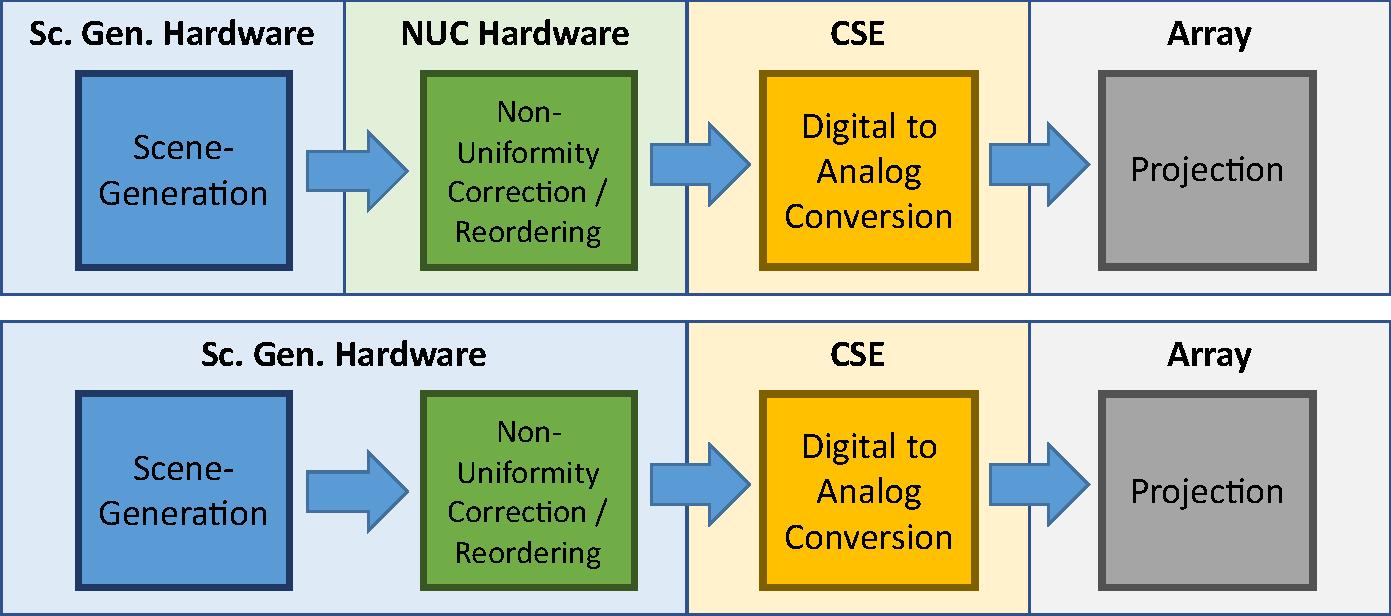
\includegraphics[width=1.0\textwidth]{fig/typical_projection_system_hardware.pdf}
        \caption{Hardware Mapping of an IRLED Projection Process}
        \label{fig:typical_projection_hardware}
    \end{figure}

    Given that these processes are separate, they can be mapped readily to a machine model which represents an abstraction of an IRSP system utilizing the PDP as shown in Figure~\ref{fig:amm}. The Abstract Machine Model (AMM) separates the system operation of an IRSP system into three main components scene generation, compositing, and display. Scene generation consist of image generation just as in traditional IRSPs; however, more than one scene generator can be utilized to generate partial imagery. Compositing is the process of combining partial images into full PDP frames as well as performing non-uniformity correction and data reordering. More than one compositor is allowed for the purposes of scaling. an IRLED Array tile represents both an array tile and its supporting electronics. Between the components exist abstract links which operate using the PDP. Compositor blocks and IRLED Array Tiles have a one-to-one relationship. The multiple CSE setup discussed in Chapter~\ref{sec:array_Interleaved_write_process} is an example of this type of setup.

    \begin{figure}
        \centering
        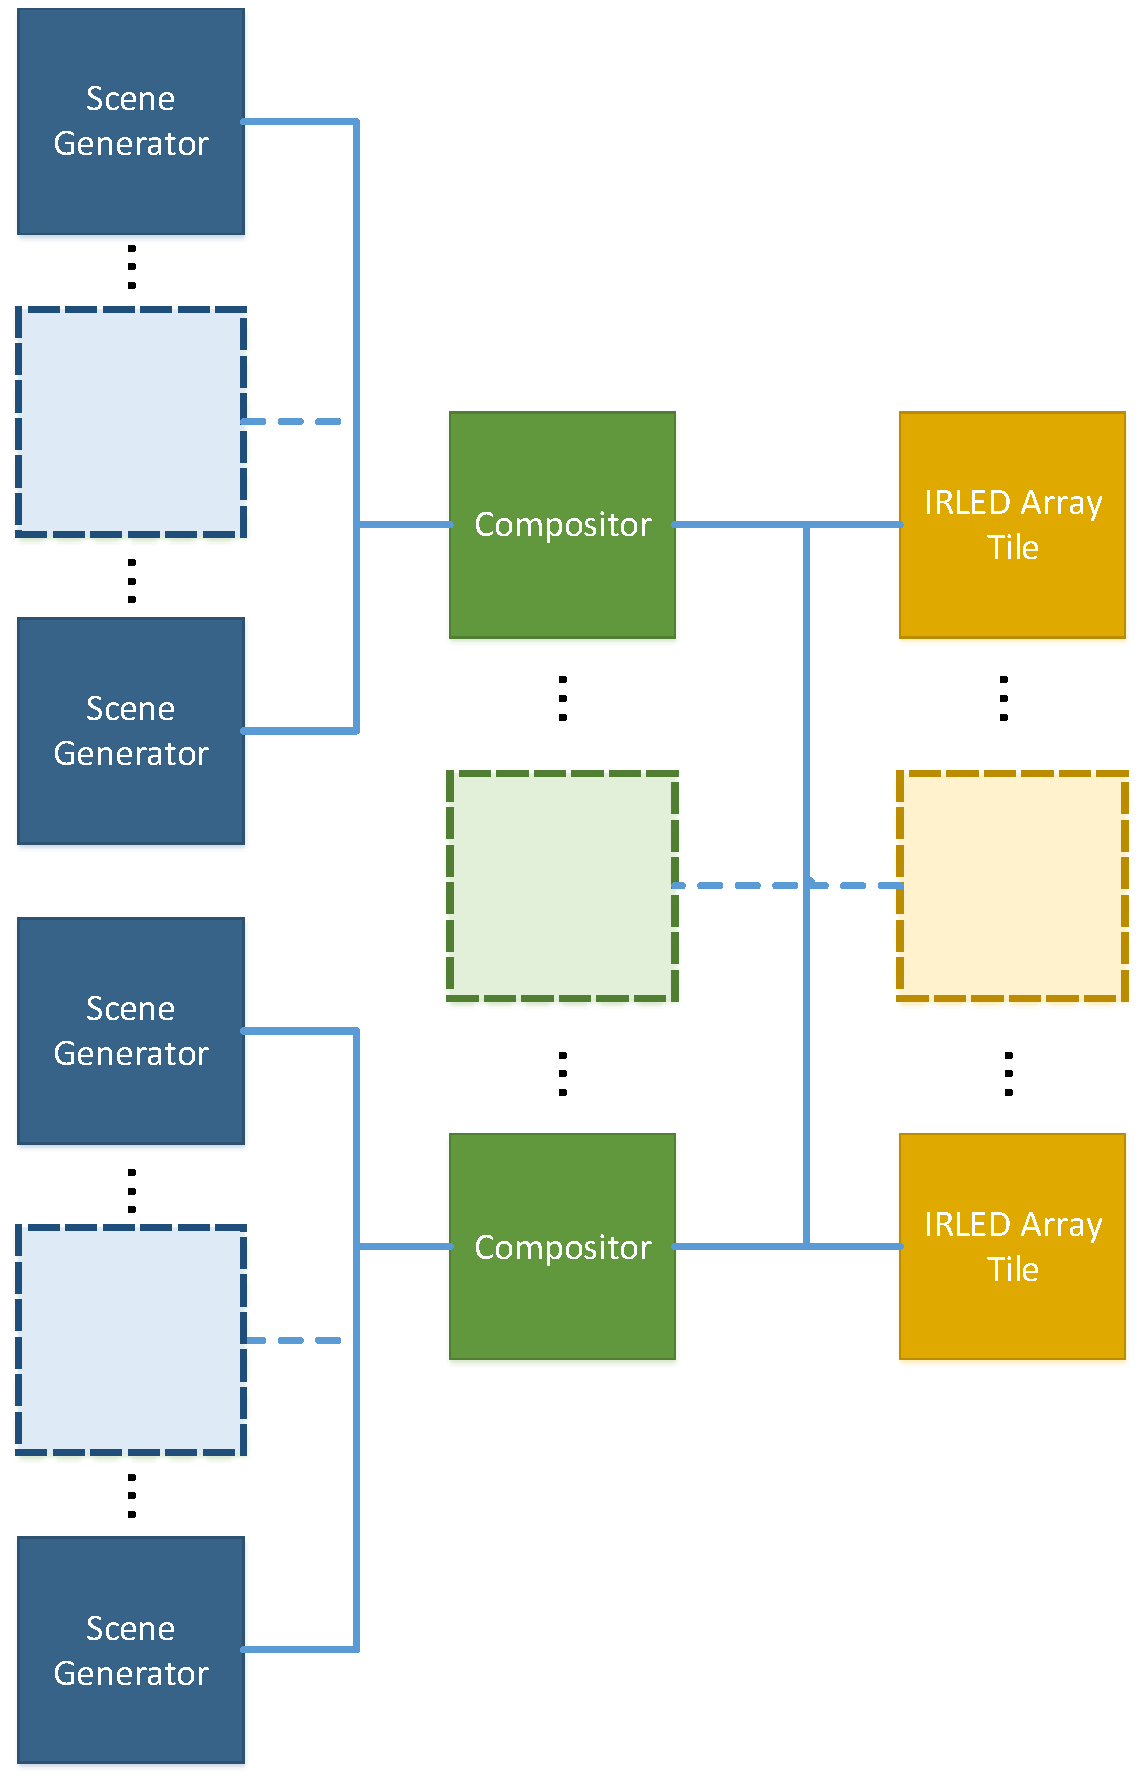
\includegraphics[width=0.83\textwidth]{fig/amm.pdf}
        \caption{Abstract Machine Model of the PDP architecture with 1-to-N relationships between components}
        \label{fig:amm}
    \end{figure}

    The relationship between these components remains abstracted in such a way that hardware components may be scaled to fit demand. At its most basic, a single scene generator, compositor, and IRLED array tile may be used just as in a traditional setup. For higher speed requirements, hardware components may be mapped as needed. As noted above, the links between components in the system utilize the PDP for communication, data-transfer, and synchronization. The compositing component differs from a traditional IRSP system in that it is responsible for taking imagery from many sources, possibly at different frame rates, and combining them into a single image for transmission to IRLED array tiles. This process will be discussed in more detail in the following section.

\section{Compositing}
    \label{sec:compositing}
    This section discusses a compositing layer and analysis that could be implemented into a system utilizing the PDP. As noted previously, compositing is the process of combining two or more images into a single picture. In high-speed systems imagery could be generated in individual pieces and combined via a compositor layer. This process might be done by a single system or via separate systems.

    A general example of how compositing might look is shown in Figure~\ref{fig:compositing}. During the compositing process frame segments are ranked to determine which to send at high speeds, and which to send at low speeds for intelligent bandwidth utilization. Once segmented and ranked into non-overlapping speed classes, frame segments are transmitted at the necessary rate. Figure~\ref{fig:compositing_overlayed} shows the source segments overlayed with the image where one can see how each region maps to the image.

    \begin{figure}
        \centering
        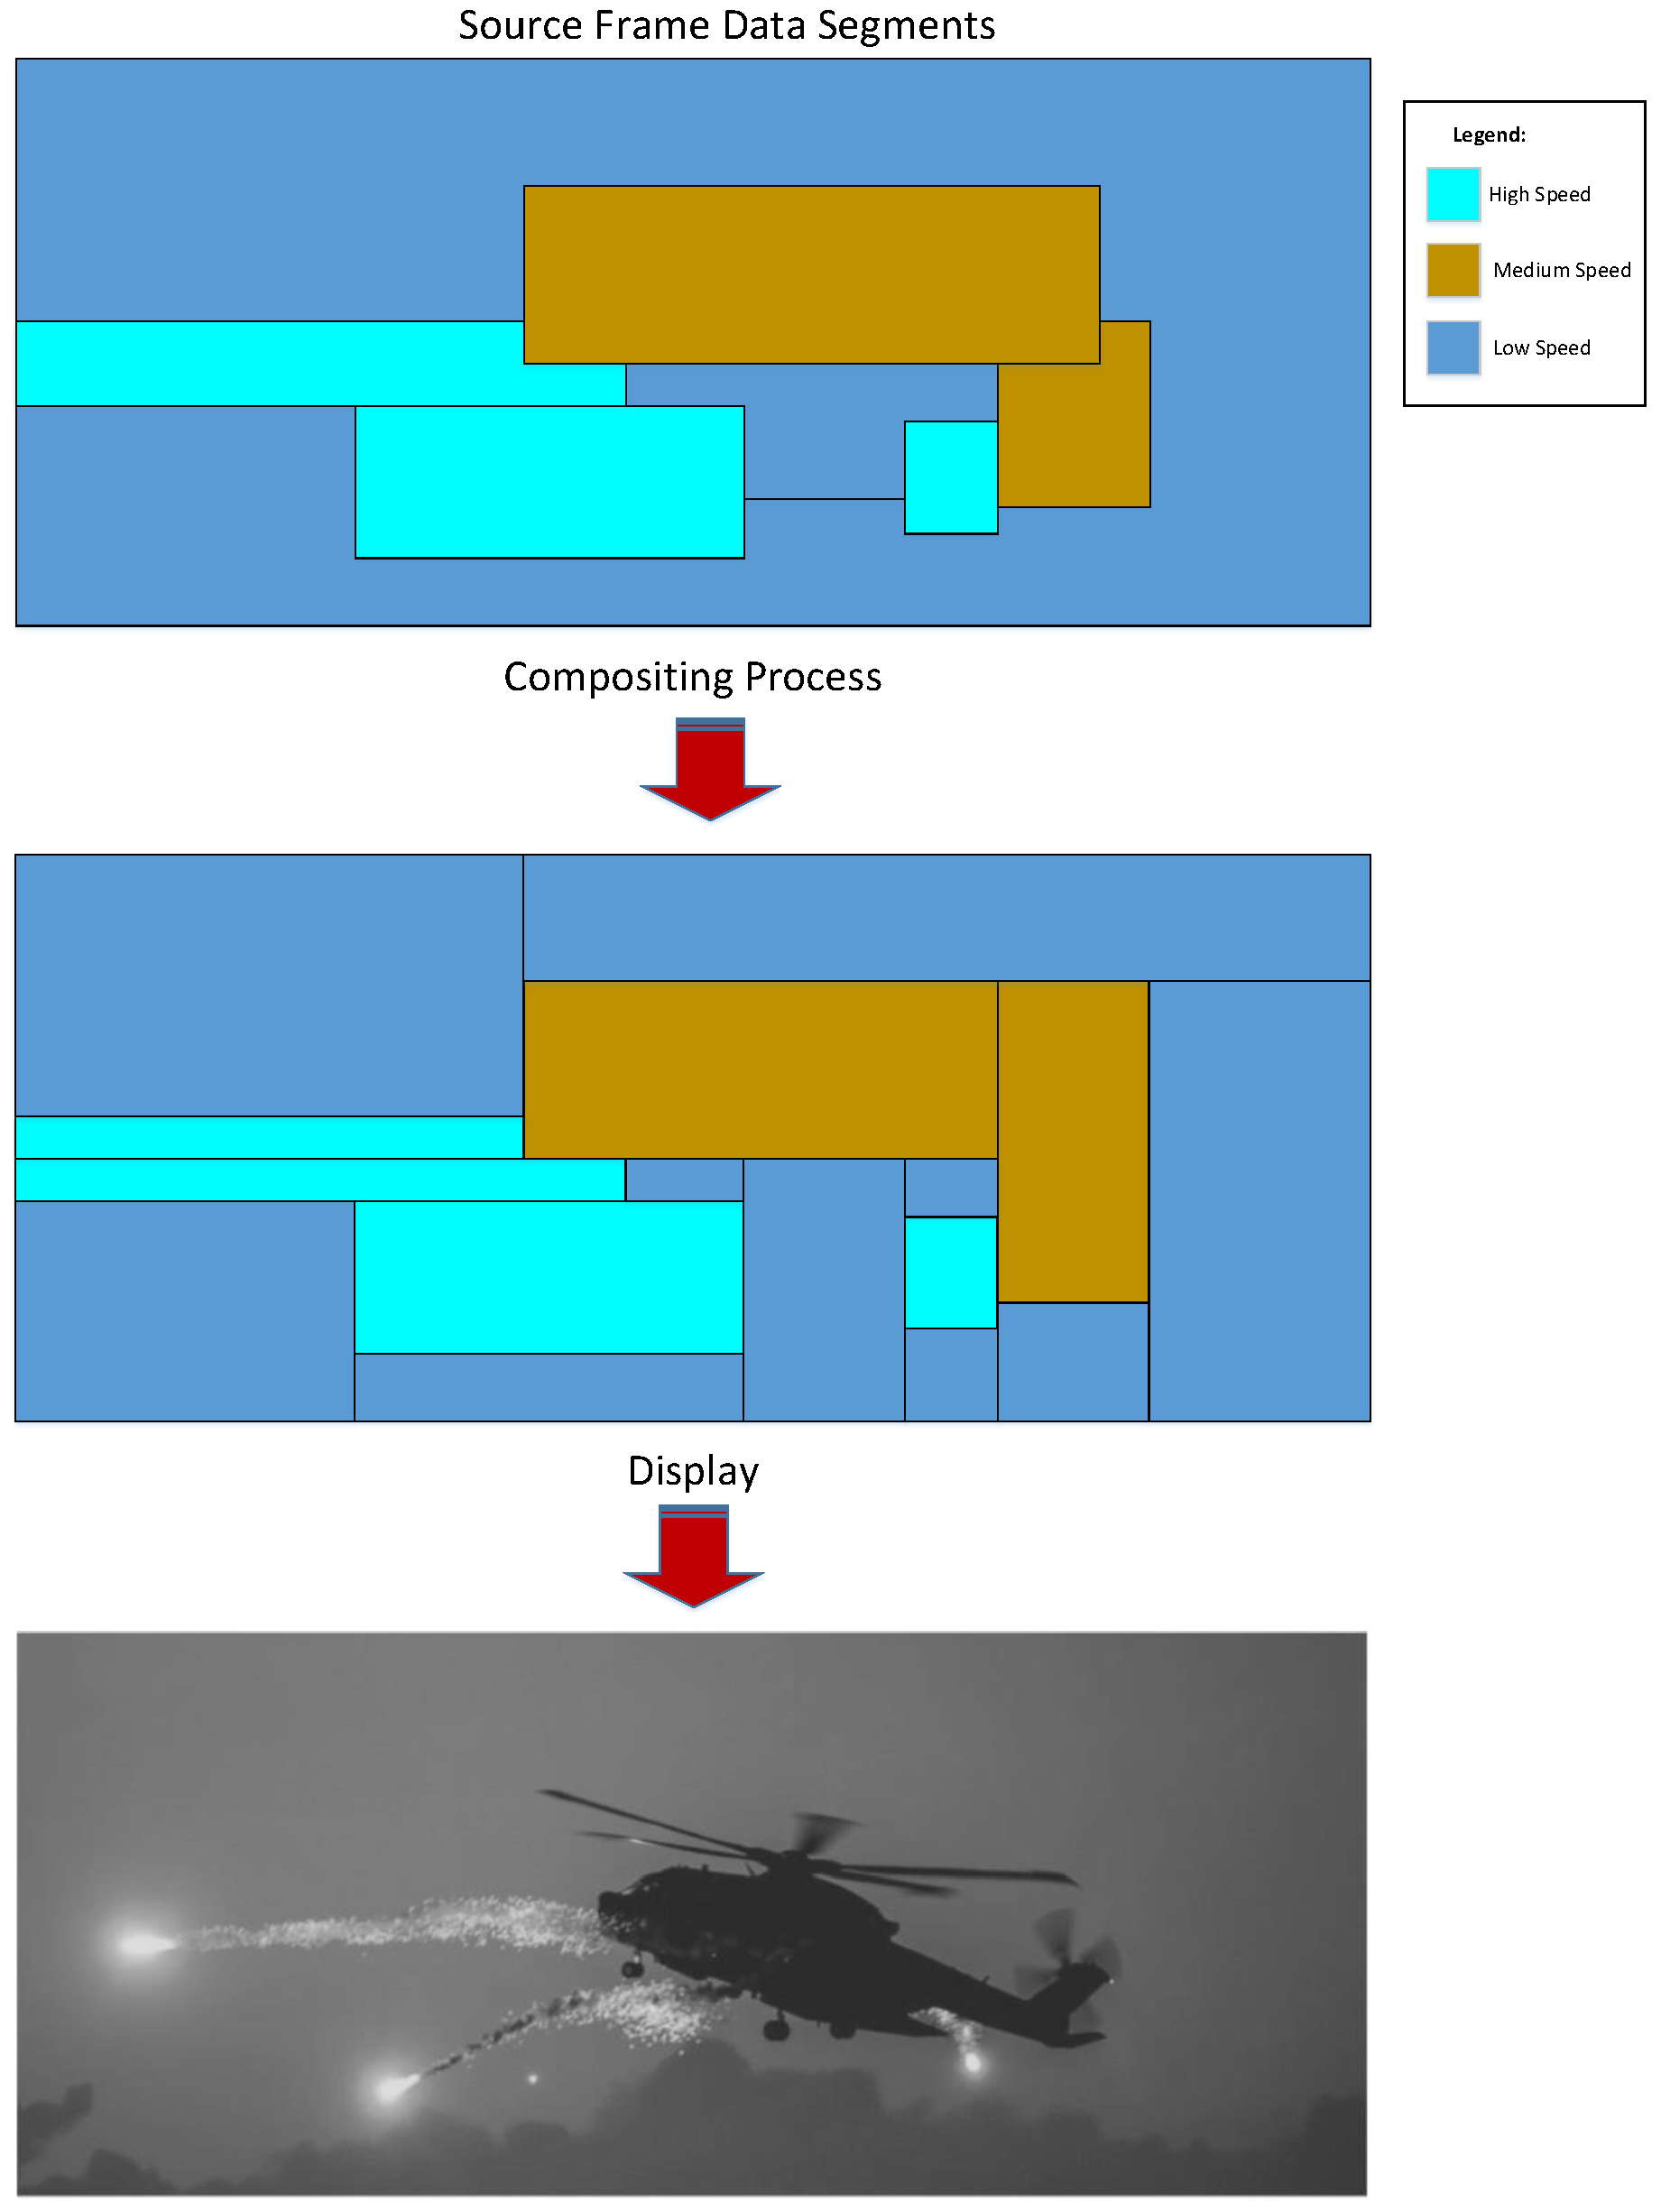
\includegraphics[width=1.0\textwidth]{fig/compositing.pdf}
        \caption{Compositing Process Example}
        \label{fig:compositing}
    \end{figure}

    \begin{figure}
        \centering
        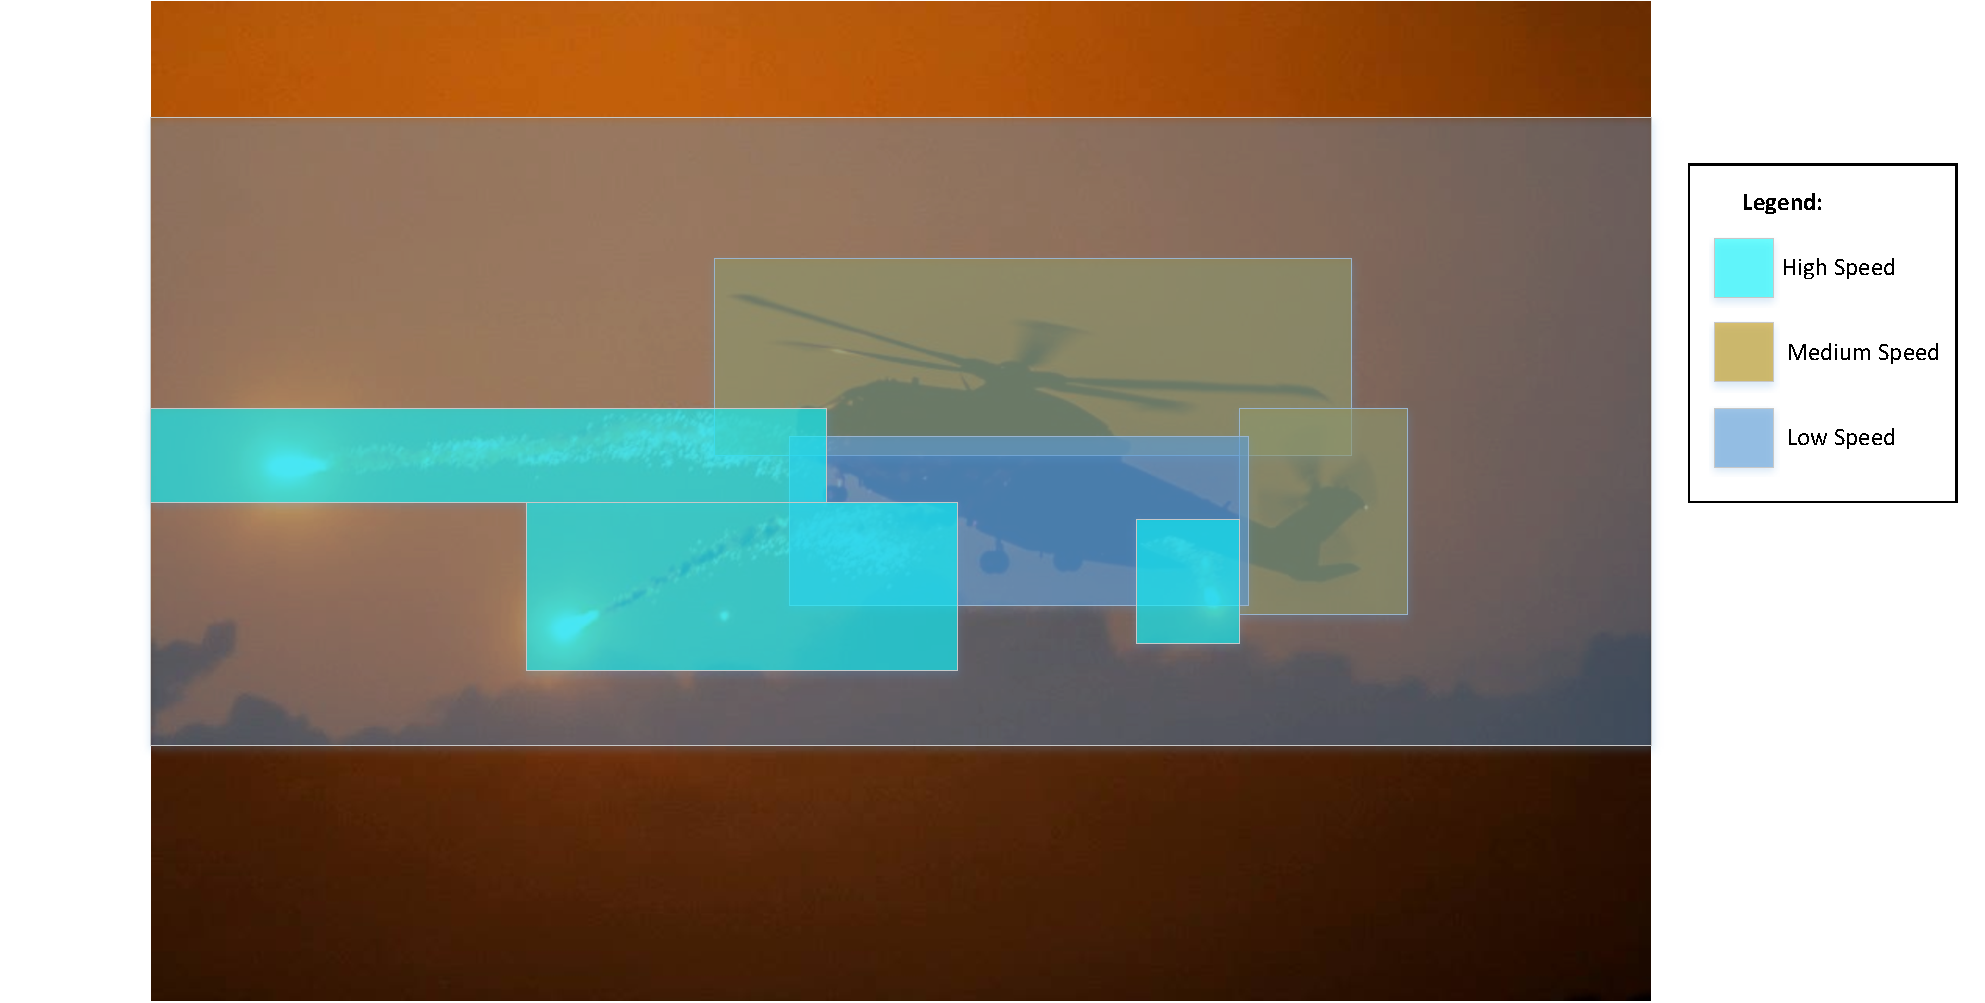
\includegraphics[width=1.0\textwidth]{fig/compositing_combined.pdf}
        \caption{Compositing Process Overlayed}
        \label{fig:compositing_overlayed}
    \end{figure}

    Consider the above scenario in the case of a single scene generator. In this case, the compositor will receive data from a single source. As frame data is received, a differencing algorithm can be employed to determine how to segment the overall frame for optimal data transfer based off the rate of change for individual portions of the frame relative to the prior frame. Portions that rapidly change will be sent more often than portions that change slowly in order to maximize bandwidth for high-speed display. This consequently also has the effect of improving the performance of the analog chain by allowing for devices to reserve more time to drive rapidly changing portions of a display over slowly changing portions. This will be discussed in more detail shortly.

    In order to demonstrate how a differencing algorithm might be employed consider Figure~\ref{fig:intensity_map} which shows a series of composited frames with segmented regions that could be sent as individual PDP draw region packets to an array. Each region is a representation of the average intensity of all pixels contained within that region. Darker regions indicate higher intensity and lighter regions lower intensity. During the compositing process of each frame, the average intensity of light output for each segment could be computed. The outlined segments for a given frame indicate a large change in intensity from the previous frame. The compositor could then assign a weight to indicate which regions have a large absolute change in intensity from frame to frame. This information could then be utilized for deciding which segments of an image to send at high-speed operation or low speed operation. Segments with larger changes in intensity would be higher priority than segments with lower changes. The PDP could be utilized to send these regions at a much higher frame rate than the more slowly changing segments to reflect the fast changes in intensity. In practice, an implementation would likely utilize a rolling weighted score where regions with higher weighted scores would be sent more frequently than regions with lower scores; with the remaining bandwidth devoted to lower regions. Regions that could not be updated in a given frame would then have their priority increased for the next frame.

    \begin{figure}
        \centering
        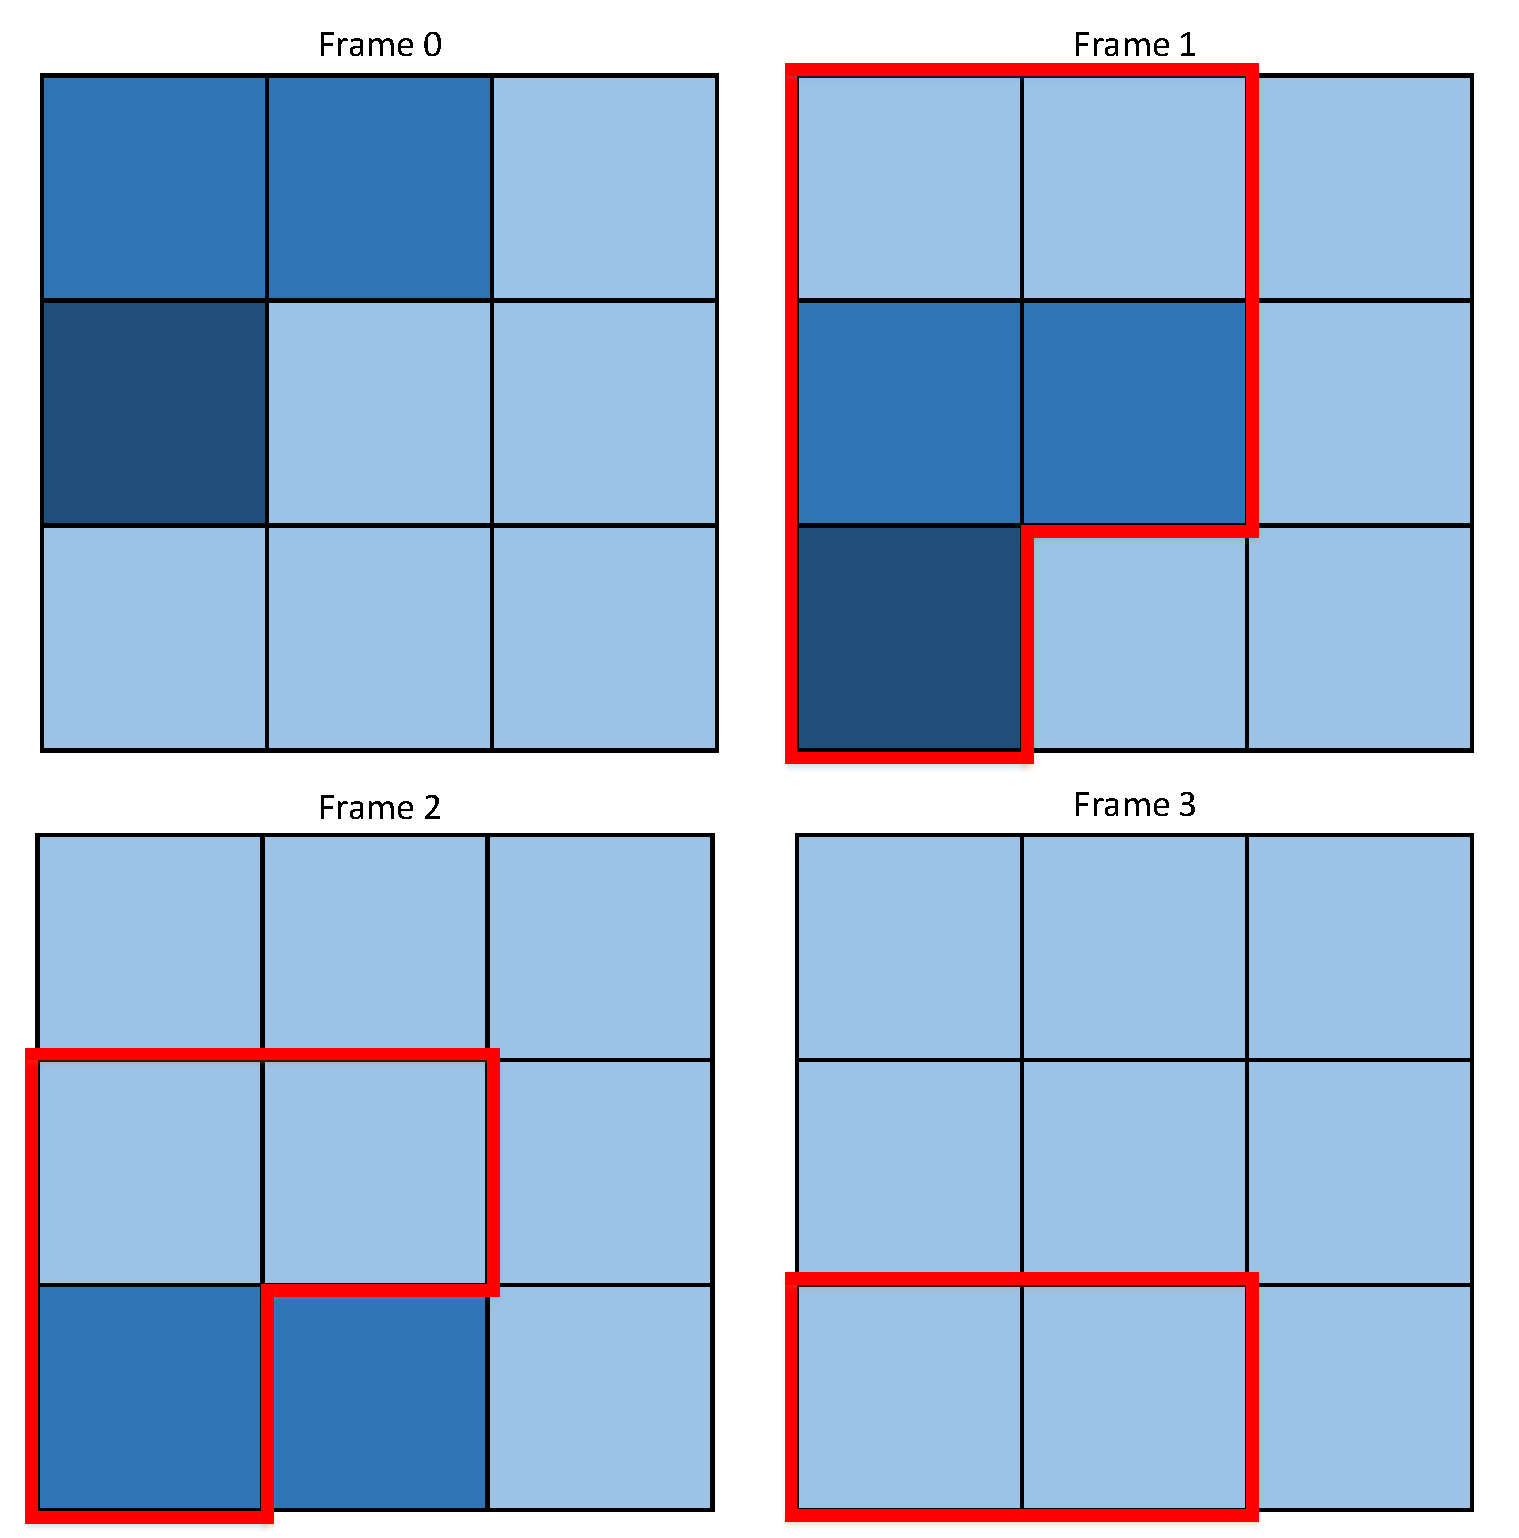
\includegraphics[width=1.0\textwidth]{fig/frames.pdf}
        \caption{Average Intensity Map of PDP Regions for Composited Frames}
        \label{fig:intensity_map}
    \end{figure}

    In a real system, frames would likely be segmented more finely than in this example, allowing for small segments to be dynamically transmitted, as necessary. This would then give the ability for fast changing data to update at rates far greater than a static fixed frame rate display would be capable of doing under the same hardware constraints. An added benefit is that by prioritizing segments, and decreasing the rates of slowly changing segments, more analog bandwidth can be utilized for drawing the high-speed portions of a display since the close support electronics no longer need to devote DAC and amplifier resources toward drawing low speed regions as often. Ultimately this would result in improved image fidelity by giving additional settling time to rapidly changing regions of an array. Though only touched upon in passing in Chapter~\ref{sec:array_Interleaved_write_process}, analog performance is of primary concern in IRSPs because a higher performance analog chain results in more consistent thermal output and an overall more thermally accurate image. Low analog performance can result in the same intensity data having different results over multiple captured frames due to DACs, amplifiers, and emitters not having the time to completely settle in high-speed operation.

    Now that all of the protocol level and abstract architectural details of the PDP have been discussed, the following chapter moves toward a discussion of an implementation of PDP on real hardware.

    \chapter{Implementation}
        \label{chap:implementation}
%FIXME: my research group's arrays?
This chapter describes the implemented FPGA version of the PDP architecture used on my research group's arrays. For the purposes of this discussion, only relevant details are included to ease the readers understanding. First, the chapter will discuss the purpose of the implemented architecture. Following this each component will be discussed at a high level. Finally, the operation of sub-components will be discussed.

The implemented architecture consists of the portion of the AMM that drives an IRLED tile (or emitter array) directly from data packets sent by a compositor. As such, it is responsible for receiving PDP packets, decoding and validating them, and drawing them to an IRLED array. This is shown in Figure~\ref{fig:overall_arch}. In the current implementation, packets are sent using an underlying HDMI protocol layer. The incoming data is synchronized across two distinct clock domains utilizing a synchronized circular buffer (SCB). The input side consists of two separate HDMI inputs in order to meet system bandwidth requirements. Each input is assumed to contain clock skew relative to the other so separate SCBs are used to synchronize these to the system domain. At a high level, individual data words of 24-bit sized values come in per HDMI cycle. These are transitioned to the system domain and stored for retrieval by the array emitter module. The array emitter module is responsible for bringing in each 24-bit word value and emptying the corresponding SCB slot. As it brings in each word, it begins to decode them into PDP commands. Once enough data is buffered for a write or reset command, it sends the data to the write buffer module which then drives an emitter directly through IO lines.

%\begin{figure}
    %\centering
    \begin{figure}%{0.50\textwidth}
        \centering
        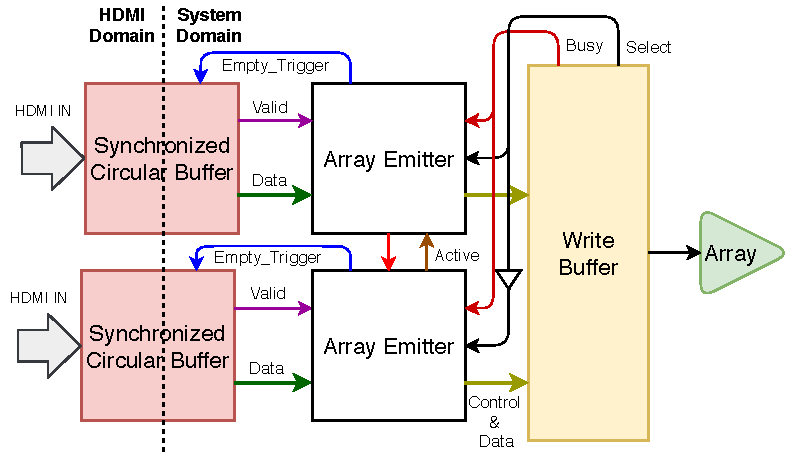
\includegraphics[width=1.0\textwidth]{fig/pdp_overall_arch.pdf}
        \caption{Overall PDP Architecture}
        \label{fig:overall_arch}
    \end{figure}%
    %\hfill
    \begin{figure}%{0.50\textwidth}
        \centering
        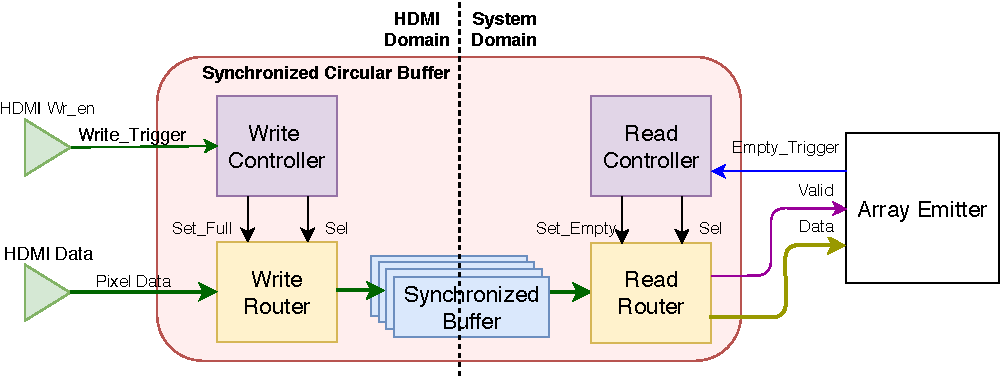
\includegraphics[width=1.0\textwidth]{fig/pdp_scb_arch.pdf}
        \caption{Synchronized Circular Buffer Architecture}
        \label{fig:scb_arch}
    \end{figure}
    %\caption{Overall Architecture \& SCB}
%\end{figure}

Figure~\ref{fig:scb_arch} shows the details of the synchronized circular buffer utilized in the implementation. Internally, it consists of two controllers, two data routers, and the actual internal buffer storage itself. The write controller is used to coordinate which internal buffer to write data to. A buffer is marked as full when a trigger comes in, and a new buffer is selected when the previous is filled. This is triggered via an external write enable signal sent from HDMI. The write router does the actual data redirection based off of the buffer selected by the write controller. Internally, a request-acknowledgment handshake is used to ensure the data has transitioned correctly across clock domains and is available on the other side. Once data becomes available, the read router will output the data lines, as well as, a valid signal indicating that the data can be read and cleared. The read controller will clear it once an empty trigger is sent from the array emitter indicating that the corresponding word has been read. It will then select the next buffer. Once the last buffer is written or read by either controller, the first buffer will be selected again. To note here for clarity, the actual filling and clearing of the buffers is done by HDMI write enable on the writer side, and the array emitter on the reader side.

Figure~\ref{fig:ae_arch} shows the details of the array emitter module used in the implementation. Internally, the array emitter consists of individual controllers that each perform a particular role. Currently these are the write enable controller, which controls writing draw region packets; the reset controller, which controls the resetting process per frame; and the valid controller which does validation checks on the input in order to verify the correctness of packets. Each controller takes in similar input signals and produces similar output signals with some exceptions depending on the actual function of the individual controller module. On the input side, each controller takes in a valid and data line corresponding to an individual word of a PDP packet. Additionally, an active line is brought into each controller to indicate whether another controller module is active or not. This is used to ensure that other modules do not become active (for correctness purposes) while another is currently processing a packet. During an idle phase, the write enable and reset controllers will wait for a corresponding packet ID to come in.

 \begin{figure}
    \centering
    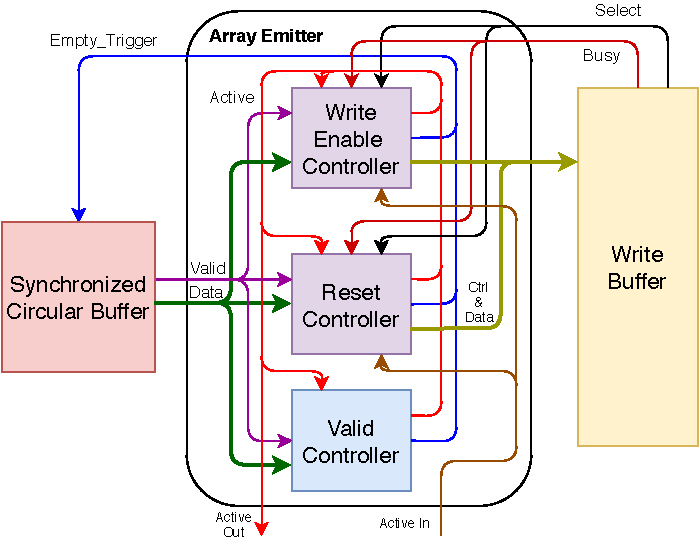
\includegraphics[width=1.0\textwidth]{fig/pdp_ae_arch.pdf}
    \caption{Array Emitter Architecture}
    \label{fig:ae_arch}
\end{figure}

When a packet ID matching an operation handled by a given controller arrives, the corresponding controller will switch states and then wait for the rest of the incoming packet data to arrive. This is shown in Figure~\ref{fig:state_machine}. For example, item 3 shows each state machine waiting for a corresponding PDP OP code. If a draw region packet ID were to arrive, then the state machine would wait for the X start address, X end address, Y start address, and Y end address shown in item 4. Finally, the state machine would buffer the needed data for a write and move to the write state once all data has been buffered. In the write state it would send the data to the write buffer. If more data needed to be written for the PDP packet, it would then continue buffering the needed data, and wait for the write buffer to be idle to send the next set of data. The busy line in Figure~\ref{fig:ae_arch} indicates when the write buffer is in the process of writing to the array. This would continue until all data was written for the packet, finally proceeding to the idle state. The reset controller contains similar logic, but for the reset process. The valid controller is used to ensure that incorrect or corrupt packet data is cleared. If an invalid packet OP code arrives during an array emitter idle phase, the valid controller will simply empty the corresponding SCB slot. In future revisions, it will perform CRC checks on packet data to ensure the header and body are valid. The Active-Out, Active-In, and Select lines are used to coordinate which array emitter module has control over the write buffer. After an array write, normally an array emitter will signal the write buffer that it is ceding control to the other array emitter, but only in cases where the other array emitter is currently active and waiting to write.

\begin{figure}
    \centering
    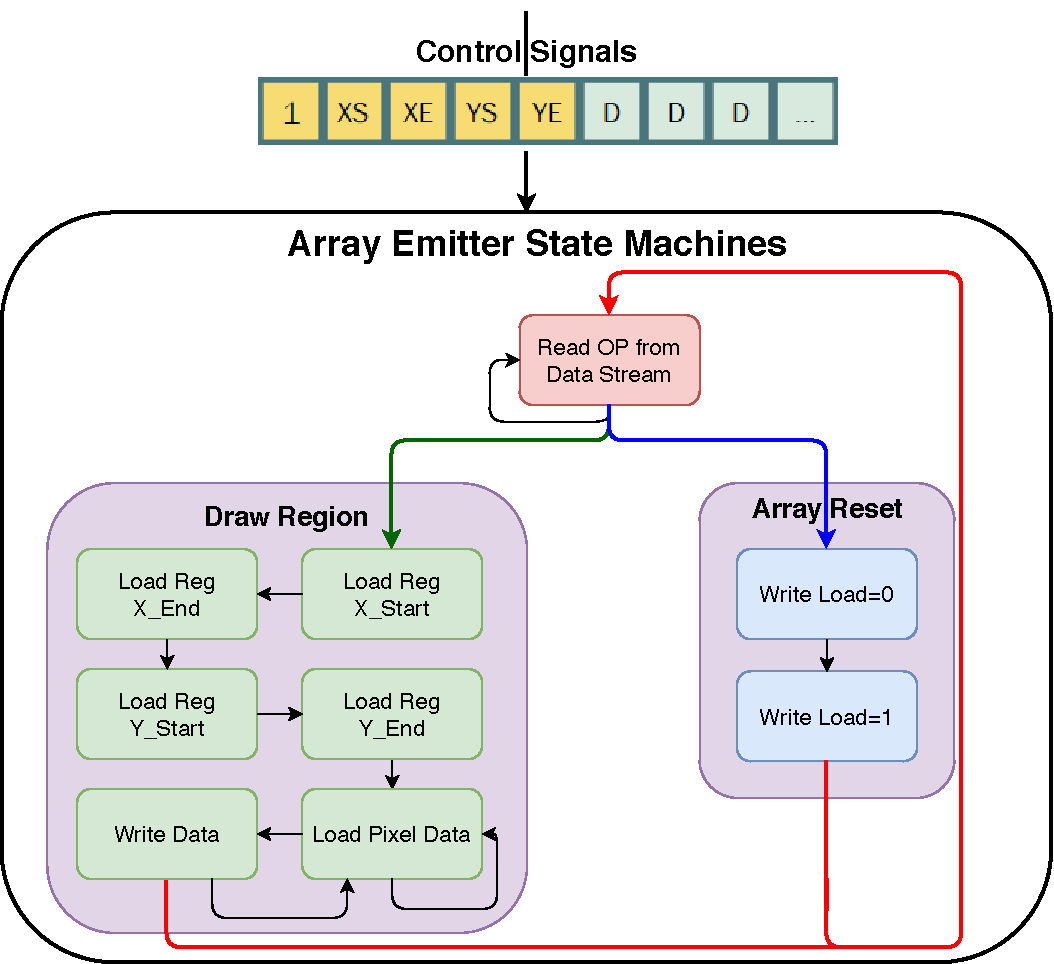
\includegraphics[width=1.0\textwidth]{fig/pdp_state_machine.pdf}
    \caption{PDP State Machine}
    \label{fig:state_machine}
\end{figure}

\section{Experimental Results}
This section provides a few captures of simulation inputs and outputs in order to show how packets arrive and are processed by the architecture.

In Figure~\ref{fig:input_example} simulated HDMI is shown. When video data enable (write enable) goes high words of data representing PDP packets start to stream in. These are indicated by Packet ID, X start, X end, Y start, Y end, and Packet Data. Each word would be stored in an SCB slot as indicated in the previous section. The final piece of data indicated is a reset packet. Note, that the data prior to Packet ID would be ignored as it does not represent a valid PDP command. It would be discarded by the valid controller.

\begin{figure}
    \centering
    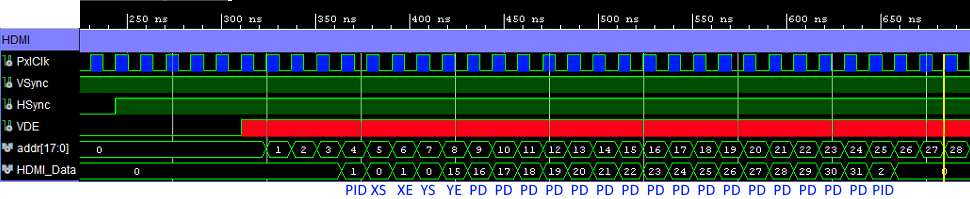
\includegraphics[width=1.0\textwidth]{fig/pdp_input_example.png}
    \caption{PDP Single HDMI Input Example Simulation}
    \label{fig:input_example}
\end{figure}

Figure~\ref{fig:output_example} shows the final output driven to the array. Highlighted in red is data from the write enable packet. Note, all values out are up shifted by 5 bits to be received by the DACs in the system. Additionally, the values are shown in reverse order from the input diagram. For example, 992 corresponds to the value of 31 on the input side. In purple the reset packet is shown with two stages of array writes. In the first stage, load line goes low. In the second stage the load line goes high.

\begin{figure}
    \centering
    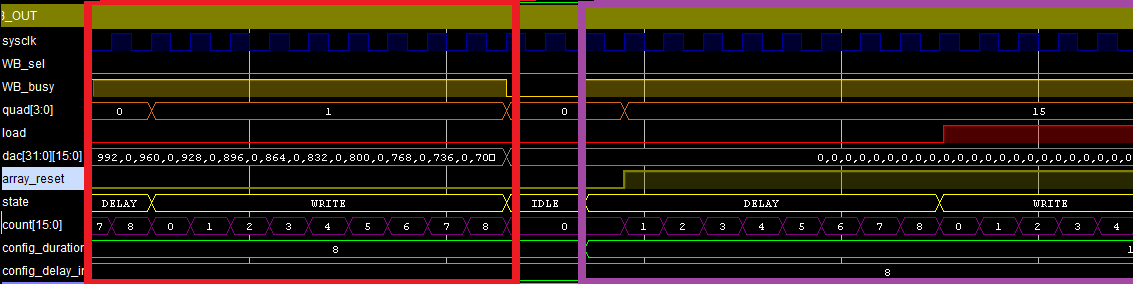
\includegraphics[width=1.0\textwidth]{fig/pdp_output_example.png}
    \caption{PDP Output Example Simulation}
    \label{fig:output_example}
\end{figure}

    \chapter{Experimental Results}
        This section provides a few captures of simulation inputs and outputs in order to show how packets arrive and are processed by the architecture.

In Figure~\ref{fig:input_example} simulated HDMI is shown. When video data enable (write enable) goes high words of data representing PDP packets start to stream in. These are indicated by Packet ID, X start, X end, Y start, Y end, and Packet Data. Each word would be stored in an SCB slot as indicated in the previous section. The final piece of data indicated is a reset packet. Note, that the data prior to Packet ID would be ignored as it does not represent a valid PDP command. It would be discarded by the valid controller.

\begin{figure}
    \centering
    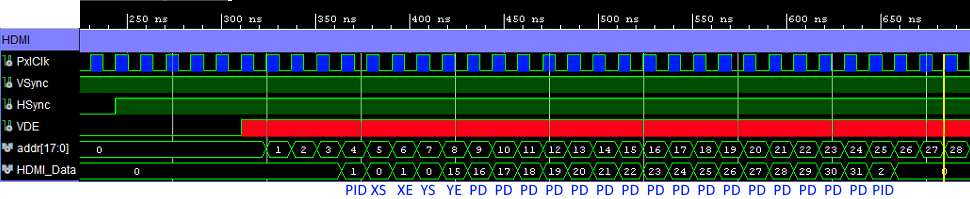
\includegraphics[width=1.0\textwidth]{fig/pdp_input_example.png}
    \caption{PDP Single HDMI Input Example Simulation}
    \label{fig:input_example}
\end{figure}

Figure~\ref{fig:output_example} shows the final output driven to the array. Highlighted in red is data from the write enable packet. Note, all values out are up shifted by 5 bits to be received by the DACs in the system. Additionally, the values are shown in reverse order from the input diagram. For example, 992 corresponds to the value of 31 on the input side. In purple the reset packet is shown with two stages of array writes. In the first stage, load line goes low. In the second stage the load line goes high.

\begin{figure}
    \centering
    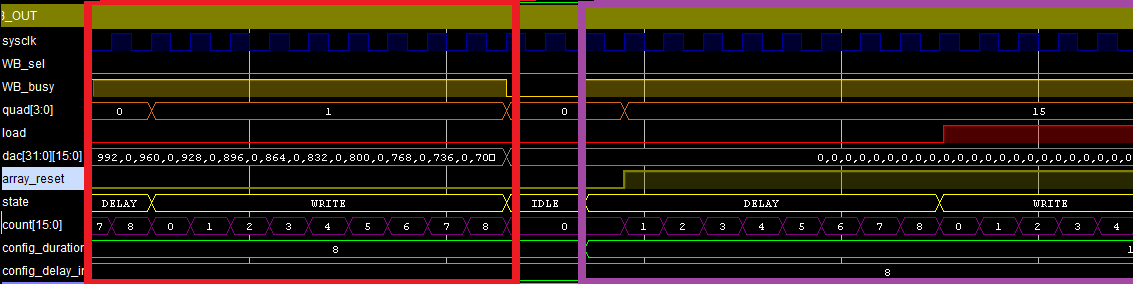
\includegraphics[width=1.0\textwidth]{fig/pdp_output_example.png}
    \caption{PDP Output Example Simulation}
    \label{fig:output_example}
\end{figure}

    \chapter*{Conclusion}
    \addcontentsline{toc}{chapter}{conclusion}
        %FIXME: remove "we"
\label{chap:conclusion}
In this paper, we described a packetized display protocol architecture and associated abstract machine model to convey the limitations in current fixed frame technology. Additionally, we provide an alternative display architecture that eschews with the design decisions of current technology to provide intelligent dynamic bandwidth utilization, fine-grained control over frame transmission and synchronization as well as allows for dynamically changing intra-frame rates. We believe this architecture has the potential to provide the capabilities to bridge the performance gap found in current technology, and will serve as a better-fit solution for future high performance IRSP systems due to the scalable nature of the design and the carefully incorporated abstraction tailored to allow for different types of hardware and system setups to utilize the PDP architecture. Care has been taken in the design to incorporate many different possible system setups without limiting the use case of PDP to a specific hardware setup; while at the same time, considering firmware implementation and timing aspects to packet decoding.

Current work includes a FPGA based implementation of a PDP decoder architecture utilizing HDMI. We have provided a description of the implemented architecture as well as simulated sample data running on the architecture. Future work includes testing the architecture on an emitter array, performing scalability testing, and comparing the results to a conventional architecture at matching pixel clock rates to show effective speedup with varying packet sizes. Further work is to be done to demonstrate dynamic frame rates in action on an array. Finally, a CRC is to be implemented to ensure correct operation at all times. We also wish to scale the number of inputs to increase the effective hardware bandwidth further than capable with a conventional system.


    \renewcommand{\bibname}{References}
    \pdfstringdefDisableCommands{\let\uppercase\relax}
    \bibliography{bib/biblio}
    \bibliographystyle{unsrt}


\end{document}
